% !Mode:: "TeX:UTF-8"
% !TEX program = xelatex
\documentclass[thesis]{skythesis}
\graphicspath{{preface/figures/}{thesis/figures/}}  % 图路径
\skip\footins = 5mm plus 4pt minus 2pt
\usepackage{pifont}
\usepackage{tikz}
\usepackage[all,pdf]{xy}
\newcommand{\Step}[1]{\textbf{Step#1}}
\newcommand{\refa}[1]{\textbf{算法} \ref{#1}}
%\usepackage{tikz}
\usepackage{pgfgantt}
\usepackage{fancyvrb}
\begin{document}
%% 信息填写
%论文题目:{中文}
\skytitle{多品种装配车间调度研究}
%论文英文题目:
\Skytitle{A study of multi job in assembly shop}
%作者:{中文姓名}{学号}
\skyauthor{陈晟恺}{201002750102}
%拼音
\Skyauthor{CHEN Sheng-kai}
%指导教师:{导师中文名}
\skymentor{鲁建厦、董巧英}
%拼音
\Skymentor{LU Jian-sha, Dong Qiao-ying}
%个人信息:{毕业年份}{专业}
\skyinfo{2014}{工业工程}
%班级
\skyclass{健行1001}
%学院信息:{学院中文}
\skycollege{健行学院}
%英文信息
\Skycollege{Jianxing Honor College}
%学校名称:
\skyschool{浙江工业大学}
%英文校名
\Skyschool{Zhejiang University of Technology}     % 个人信息
% !Mode:: "TeX:UTF-8"
% !TEX root = ..\Literature_Translation.tex
%% 封面
%% 信息填写
%论文题目:{中文}
\skytitle{多品种装配车间调度研究}
%论文英文题目:
\Skytitle{A study of multi job in assembly shop}
%作者:{中文姓名}{学号}
\skyauthor{陈晟恺}{201002750102}
%拼音
\Skyauthor{CHEN Sheng-kai}
%指导教师:{导师中文名}
\skymentor{鲁建厦、董巧英}
%拼音
\Skymentor{LU Jian-sha, Dong Qiao-ying}
%个人信息:{毕业年份}{专业}
\skyinfo{2014}{工业工程}
%班级
\skyclass{健行1001}
%学院信息:{学院中文}
\skycollege{健行学院}
%英文信息
\Skycollege{Jianxing Honor College}
%学校名称:
\skyschool{浙江工业大学}
%英文校名
\Skyschool{Zhejiang University of Technology}
\thispagestyle{empty}
\pdfbookmark[0]{封~~面}{thesiscover}
\phantomsection \label{thesiscover} %无形节命令
\newcommand\midtitle{}

\ifskythesis
  \renewcommand\midtitle{毕业论文(毕业设计说明书)}
\fi
\ifskylandt
  \renewcommand\midtitle{毕业论文(文献综述、外文翻译)}
\fi
\ifskyproposal
  \renewcommand\midtitle{毕业论文(开题报告)}
\fi
\vspace*{10mm}
% 校名
\begin{center}
   
\includegraphics[height=42pt,trim= 0 300 0 0]{zjutlogo}{\stxingkai\juhao{~浙江工业大学}}
\end{center}
\vspace*{12mm}
\centerline{\linespread{1.5}\yihao\bfseries\fangsong\midtitle}
\vspace*{19mm}

\renewcommand{\arraystretch}{1.0} %列表行距
\hspace*{3mm} 

{\sfzhongsong\zihao{1}{题目}
\hspace{0mm} 
\begin{minipage}[t]{120mm} % 这里建议自行微调
 \centering 
 \renewcommand{\ULthickness}{1.2pt}
 \renewcommand{\CJKunderlinecolor}{\color{black}}
   \linespread{1.1}\CJKunderline{\quad\skytitlec\quad}
\end{minipage}
}

\vspace*{15mm}
\begin{center}
    %\setlength{\arrayrulewidth}{0.5pt}
    
    {\sfzhongsong\zihao{3}
    \renewcommand{\ULthickness}{1.2pt}
    \renewcommand{\CJKunderlinecolor}{\color{black}}
    \newcommand{\kdist}{\hspace{4em}}
    
        \renewcommand{\arraystretch}{1.5}
        \begin{tabular}{lc}
            专\hspace{2em}业:& \CJKunderline{\kdist\extt{\skymajor}\kdist} \\ 
            班\hspace{2em}级: & \CJKunderline{\kdist\extt{\skyclassc}\kdist} \\
            学生姓名: &  \CJKunderline{\kdist\extt{\skyauthornamec}\kdist}\\
            指导老师: & \CJKunderline{\kdist\extt{\skymentorc}\kdist} \\
        \end{tabular}
    }
\vfill

{\sfzhongsong\zihao{4} 2013 -- 2014学年}
\end{center}

      % 封面
\frontmatter
{\pdfbookmark[0]{学位论文原创性声明}{thesisstatement}
\phantomsection
\includepdf{preface/statement}}
\pagenumbering{Roman}
%\begingroup % 在组内的chapter不换行
%\let\clearpage\relax % chapter之后不换页



%% !Mode:: "TeX:UTF-8"
%% 中文摘要
\begin{abstractc}
\begin{center}
{
\xiaosi
\vspace{1em}

 学生姓名:\skyauthornamec \hspace{20mm} 指导老师:\skymentorc

\skyschoolc\skycollegec}

{\xiaosan\bf\vbox{} \heiti {摘\quad 要}}
\vspace{-1cm}
\end{center}

{\sihao\indent

% !Mode:: "TeX:UTF-8"
本文针对某汽车电子零部件企业装配车间调度问题进行研究,该车间具有多条同质装配线,采用多品种、批量、面向主机厂的装配方式,存在提高产线利用率、降低冗余度、均衡生产等提升空间。突破主机厂限制是有效的解决方案,这是一个多品种多装配线轮番调度优化问题。

建立了$2$个调度优化模型,模型1 适用于订单到达稳定的情况,模型2 适用于不稳定的情况。两个模型都以加权拖延时间和与加权完成时刻和为主体,采用决策系数将之结合,模型2 需要考虑插单,引入和定义了产线闲置、流水线利用率、均衡率等概念以适应其情况,根据多品种和多流水线的特点,设计了相应的约束条件。在模型求解算法中,定义了虚拟序列的概念,将之与调度规则及启发式策略结合设计了交替改进(Cycle Amend, Cyc) 和虚拟序列(Virtual List, Vtr) 类多个求解算法。计算实验结果表明:Vtr -- Tabu 算法适用于中小规模的不考虑插单情况的问题,且随着工期目标的重视而凸显改进效果,VVT 算法的求解结果在多种不同决策环境下都显示出了较高的质量和稳定性。所提算法求解该模型是有效果的,所建模型也适合该问题。

本文所提的多品种多流水线轮番调度模型及其算法确实进一步提高了流水线利用率、按时交付等性能,仍存在如加入混流生产的改进空间。

\keywordsc{多品种多装配线,调度模型,虚拟序列,算法设计}
}
\end{abstractc}     % 中文摘要
%% !Mode:: "TeX:UTF-8"
%% 英文摘要
\begin{abstracte}
\begin{center}
\vspace{1em}
{\xiaosi \onehalfspacing
 Author: \Skyauthorc\hspace{20mm} Mentor: \Skymentorc

\Skycollegec, \Skyschoolc

{\xiaosan\bf\vbox{} Abstract}
}
\end{center}

{\indent \sihao % !Mode:: "TeX:UTF-8"
Multi-type massive production usually takes part in the assembly line of electronic parts for auto-mobile, however, a myopic way that specialize assembly line by the main factories is widely used, so that low utilization , high redundancy and unbalance production always happens. A sound solution is to despecialize the assembly line, the implementation of this solution is a so called multi-type multi-assembly-line take-turn scheduling problem. In this study, 2 mathematical models is built for different levels of managenent to apply. With proposed concept of \textit{virtual list}, schedule rule and heuristic tactic, 5 algorithms: Cyc --ATC, Cyc -- ATCS, Cyc -- Tabu, Vtr -- Tabu, VVT in 2 classes are designed. Experiment takes with script in Python shows, that Vtr -- Tabu algorithm suits for small and median scale problem, especially for none-job-inseting high weighted date-related problem, while high stability and quality schedule in various aspects can be obtain with VVT algorithm.

\keywordse{~multi-type, multi-assembly-line, scheduling model, virtual list, algroithm design}}
\end{abstracte}
     % English Abstract
{\pdfbookmark[0]{目~~录}{thesiscontent}
\phantomsection
\singlespacing\tableofcontents           % 中文目录
\listoffigures             % 图目录
\makeatletter
\@starttoc{lof}
\@starttoc{lot}
\makeatother
%\listoftables              % 表目录
}

%%%%%%%%%% 正文 %%%%%%%%%%
\mainmatter
\makeatletter
%\include{body/intros}
% !Mode:: "TeX:UTF-8"
% !TEX root = ..\Literature_Translation.tex
%%  绪论
\chapter{绪论}
\section{课题研究的背景和意义}
本文的研究对象是汽车零部件装配生产线,是典型的多品种小批量生产方式,并且在需求日益多样化的背景下,时常要根据产品调整生产。本文将从这种生产方式着手研究多品种产品的装配生产调度问题。

\subsection{课题研究背景}
汽车装配大多采用同步装配流水线方式作业,将装配过程分为多个作业单元,并安排在流水线的相应工位上,
车体在移到中装配,各工位同时作业。以往,汽车装配工厂固定地生产一种或少数几种车型,采用大批量、规模化的生产。然而,随着技术的日新月异,客户需求的多样化,以及精益思想、环保节能观念的出现,汽车工业的生产模式不得不转变为面向订单的小批量、多品种的生产方式。因此,缩短交货期、提高资源利用率、降低生产成本、提高生产运作的灵活性,已成为保证企业市场竞争力的重要手段。

多品种装配是在基本不改变或较少改变现有生产设施的前提下,通过对装配生产线的合理组织与调度优化,实现多品种共线装配,以最大限度地挖掘生产线的潜能,向客户提供定制的个性化产品和服务。

生产调度就是组织执行生产进度计划的工作,作为一种决策形式,调度在制造业扮演者至关重要的角色,尤其在现今充满竞争的环境下,有效的生产调度已成为能在市场竞争下生存的必须。

从上个世纪50年代起,调度问题的研究就受到应用数学、运筹学、工程技术等领域科学家的重视,科学家们利用运筹学中的线性规划、整数规划、目标规划、动态规划及决策分析方法,研究并解决了一系列有代表意义的调度和优化问题\cite{徐俊刚2004生产调度理论和方法研究综述}。

如今,随着计算机的发展,信息技术的成熟,许多过去只在理论层面上的调度算法,都可以通过计算机辅助得以验证与运用,给制造业的具体实力提升带来了可能。

\subsection{课题研究意义}
提高竞争力的方法有很多,对于汽车工业,产品需求多样化和市场细分化,促使越来越多的制造商将多品种装配作为增强其竞争能力的有效手段。具体来说,对于汽车零部件,装配过程主要是以零部件的安装、紧固为主,其次是联接、压装和加注冷却液、制动液等液体以及整车质量检测的工序,有时还要根据用户意向选装。因此,合理安排装配产线,优化调度作业单元,对保证汽车装配质量,快速响应需求,提高汽车装配线的生产效率有着重要的现实意义。

而实现多产品装配不仅需要技术上的支持,也需要有理论来实践。虽然在Henry Gantt 的那个时代起,调度的理论研究就受到了制造业的关注,然而生产模式的转变,信息技术的出现,都使得一些过去经典的调度算法不再适用,这就需要我们来修正那些方法,或者发展新的算法,本课题便是以此为中心。

举例来说,随着调度问题的规模增大,人们发现即使通过计算机,有些问题的算法并不是有效的,因为它们的求解超出了可接受的运行时间。逻辑学家和计算机科学家通过研究这类问题,建立了复杂度理论,并称这些问题是$NP$问题,问题的复杂度会是随着问题规模增大呈现指数爆炸。如果能从汽车行业的零部件装配调度出发,研究出通用的算法,那就间接证明了$P=NP$,可谓意义非凡。然而本课题重点不在此,这个问题对于作者来说难度太大。

这样一来,有时得到最优调度或者最优解的成本就变得太高了,那么近似最优解便成了很好的选择。然而调度问题的算法本来就众多,求解近似最优解更是如此,不同的算法适用的情况也不尽相同。因此,从多品种装配着手研究调度算法,对增加产品多样性,加快需求响应速度,加快提高企业的竞争力有着重要意义。

\section{课题研究的国内外现状}

你面向的对象是汽车零部件装配线  然后你的调度是有几个目标的 可以从对象和目标入手来写
同时也可以参考一些相关的硕士论文和博士论文 看他们的研究背景意义怎么写的
\subsection{国内研究状况}

\subsection{国外研究状况}
装配车间的生产调度决定了产品能否准时交货,某企业装配车间有多条装配线,每条装配线可分时轮番生产不同品种的产品,为了管理方便,按照产品所属厂家来安排组织生产,但这种方法存在负荷不均衡、换线损失等问题。课题对现在存在的问题进行分析,对所有需要生产的产品进行筛选组合,设计新的调度方案,以期获得均衡的生产线利用率、减少换线时间浪费、缩短完工时间、降低生产成本
% !Mode:: "TeX:UTF-8"
% !TEX root = ..\thesis.tex
\chapter{研究对象现状与分析}
本文以某汽车电子有限公司的装配车间为研究对象,进行调研。本章将介绍该公司车间的基本情况,并对现有装配线调度情况进行初步分析。
\section{公司基本情况}
该汽车电子有限公司主要产品为车用电子电器开关、控制模块、控制面板等,是美国通用、德国大众、一汽大众、上海大众、上海通用、上海汽车、长安福特、北京现代、一汽轿车、奇瑞汽车、哈飞集团等国内外40余家汽车主机厂的专业定点配套供应商,配套的代表性车型有奥迪A6(L)、奥迪A4(L)、奥迪Q5、迈腾、君越、宝来、帕萨特、奔腾、红旗、马自达M6、景程、荣威、明锐、凯越、捷达、桑塔纳等系列轿车,以及卡车、轻型车、微型车等,产品型号达6000余种。

\section{装配车间作业}
该公司的制造部分为制造一部和制造二部,制造一部主要是负责零部件的生产,不是本课题的主要研究对象;制造二部主要是负责产品总装,共8个车间,均是流水线作业,是本课题的研究对象,其相关信息如\reft{tab:2jobshopinfo}所示(单位:个)。
\begin{table}[htbp]
  \centering
  \caption{制造二部装配车间信息}
    \begin{tabular}{cccccccccc}
    \toprule
    \multicolumn{2}{c}{车间 } & 1车间   & 2车间   & 3车间   & 4车间   & 5车间   & SGM车间 & 通用车间  & 电子车间 \footnote{包括:模块线、插件线及SMT线三个部分,其中,模块线是总装线,共5条装配线,插件线和SMT线是零部件生产线。本次研究的重点是总装线,故电子车间只列出了部分信息。} \\
    \midrule
    \multicolumn{2}{c}{班 组 数 量} & 6     & 6     & 6     & 5     & 4     & 4     & 6     & 2 \\
    \multicolumn{2}{c}{流水线数量} & 7     & 7     & 7     & 6     & 7     & 6     & 5     & 5 \\
    \multicolumn{2}{c}{PMC分配品种数} & 777   & 557   & 186   & 196   & 334   & 29    & 76    & 83 \\
    \bottomrule
    \end{tabular}
  \label{tab:2jobshopinfo}
\end{table}

每个总装车间均有多条生产流水线,为方便管理,每条流水线负责各自对应主机厂的装配生产。当主机厂需要多个品种的产品时,流水线根据订单顺序进行装配作业,即同一主机厂的产品在一条生产线上轮流生产。

该公司采用面向订单生产,订单从接受到交付的流程如\reff{fig:orderflow}所示,其中虚线框内为装配车间的作业。在没有订单或者订单较少时,为了不让生产线停下来,需要进行工厂内部的计划生产,而订单较多时需要加班作业。
\begin{figure}[h]
\centering
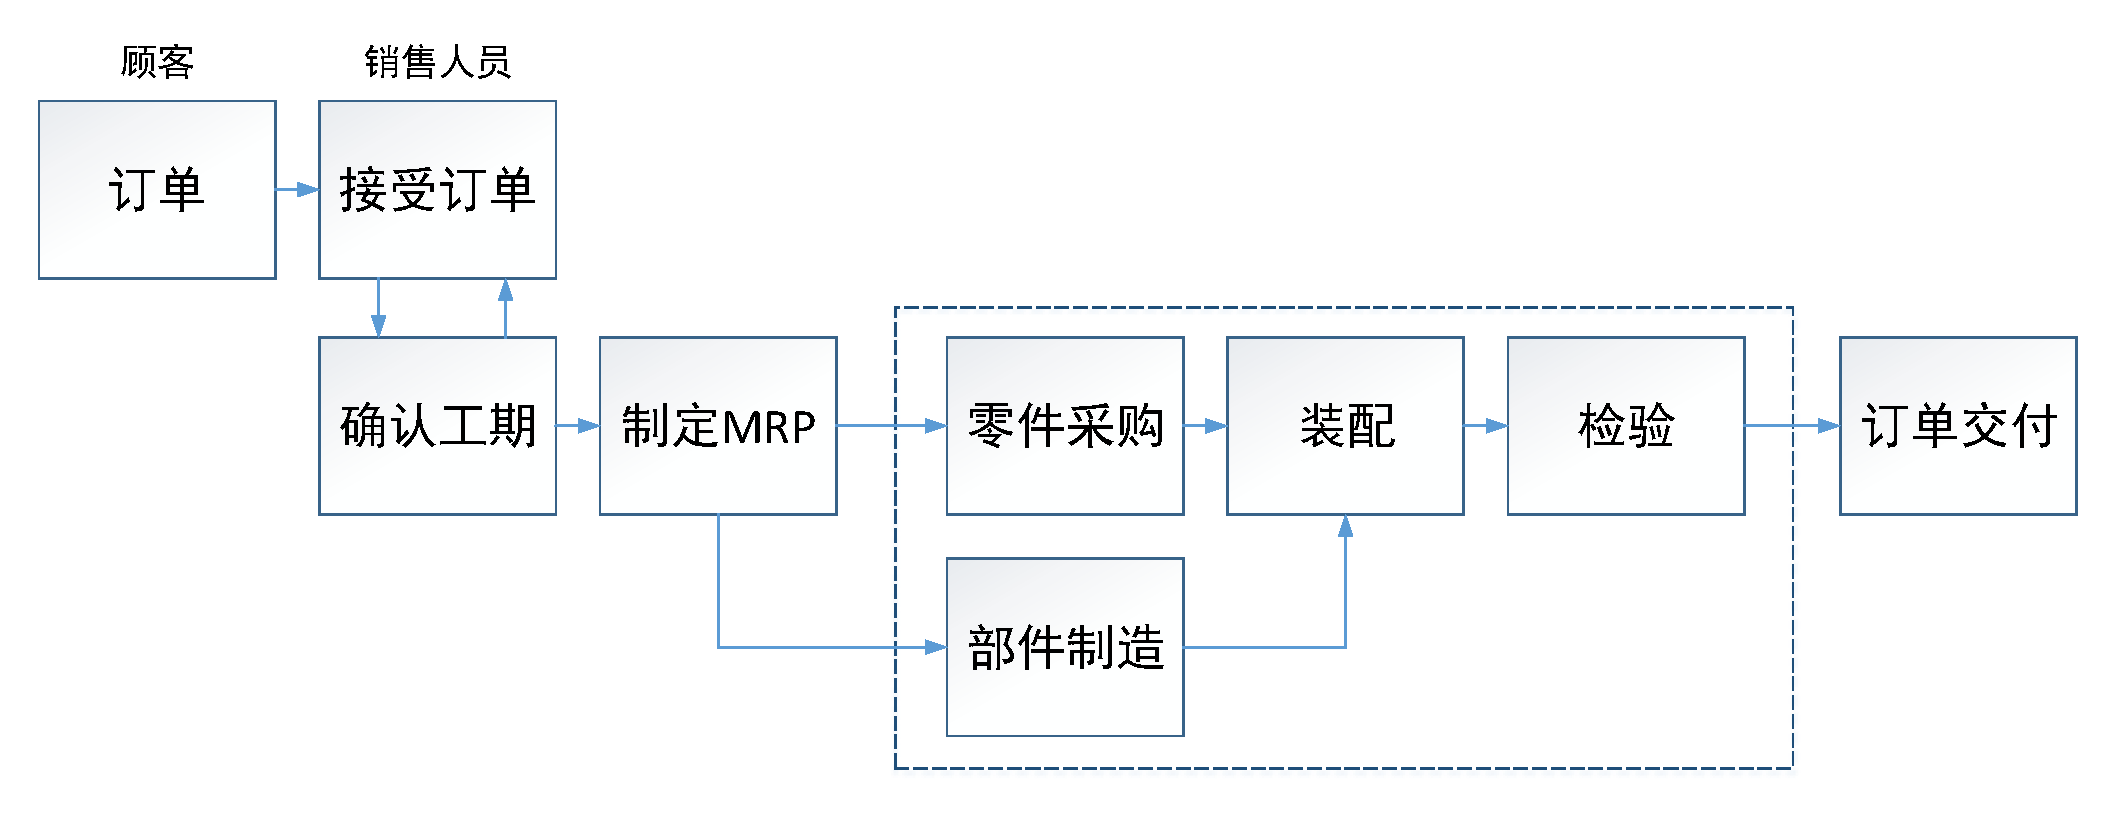
\includegraphics[width = 13cm]{orderflow.pdf}
\caption{现行订单信息流\label{fig:orderflow}}
\end{figure}

\section{产线调度现状}
当前该公司装配车间采用专线生产的方式,即客户的订单在其专用的流水线上进行生产作业,当同一客户有多个订单下达时,按照先到先服务(FCFS)的规则进行装配生产安排,多条产线并行作业互不干扰。

订单或任务到达时,如果有流水生产线空闲可用,则立刻对其根据进行生产准备,然后开始装配生产。若产线在处理订单,那么将该订单安排入其专线队列中,等待前面的批量订单生产完毕再进行生产。现行调度的产线如\reff{fig:3nowschedule}所示。

\begin{figure}[h]
\caption{3条生产线的现行调度\label{fig:3nowschedule}}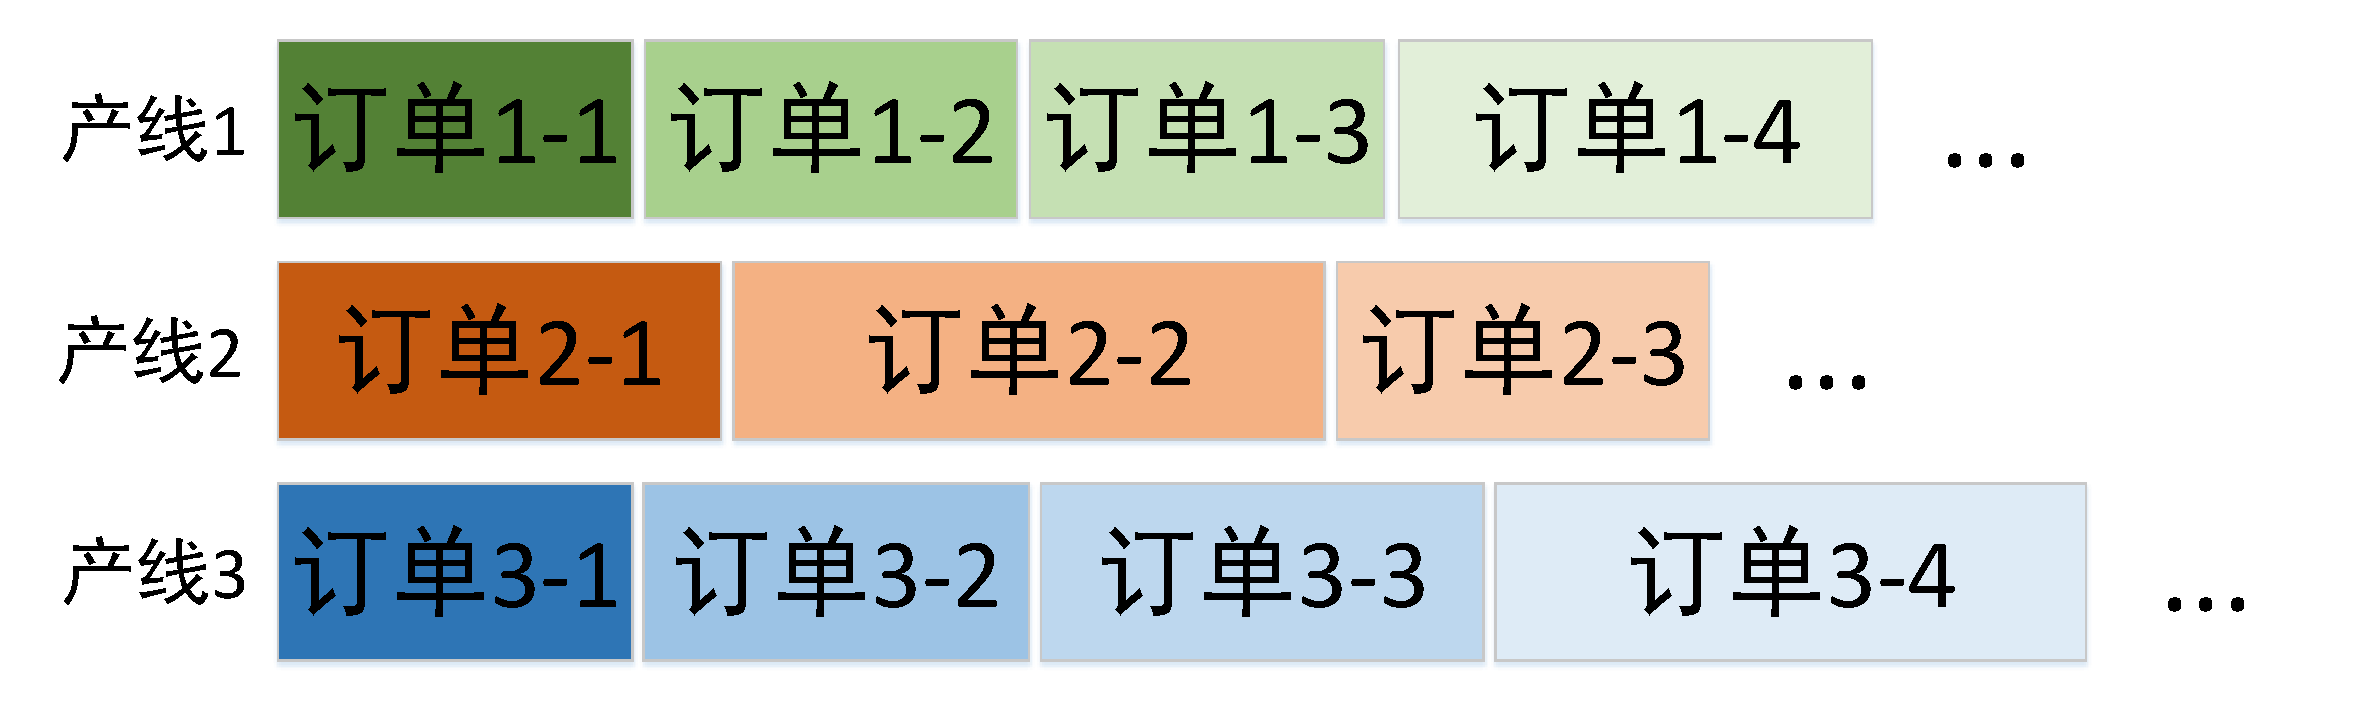
\includegraphics[width = 8cm]{orderschedulenow.pdf}
\end{figure}

现行调度方法逻辑简单,执行力强,每条装配线可分时生产不同品种的产品,而且按照厂家来安排组织生产,方便了管理。然而其缺陷也是明显的,例如常常会产生有些产线队列很长而有限产线空闲无作业,造成极大浪费。具体的现有问题将在下一章分析。


\section{生产线分析}
课题研究对象是该汽车电子公司的总装生产线,是典型的流水车间,每条流水线负责同一主机厂的不同品种产品总装流程。装配生产根据订单批量进行安排,根据先到先服务(FCFS)规则生成任务队列。

生产线分析包括上述这些差别及其产生的影响或效果,具体描述从订单、装配到交付的流程,并分析现行调度方案的一些指标。

\subsection{现行流程描述}
现行下达订单到交付的流程如\reff{fig:orderflow}所示,销售人员接到客户订单,在确认工期后,将之送达计划部门,制定主生产计划(MRP),随后根据产品特性安排采购与厂内加工。根据任务队列与批量进行产品总装,通过质检包装后,销售人员安排运输送达至客户。
订单到达会立即安排入其对应的主机厂专用产线,当同一主机厂有多个订单同时到达时,则根据最早交货期(EDD)规则进行生产调度。

本课题的研究对象是流程中的总装调度安排,
\subsection{现行调度方案}
任务下达到车间时,需要根据订单队列及其批量进行调度安排,


现行调度方案逻辑简单,执行力强,每条装配线可分时生产不同品种的产品,而且按照厂家来安排组织生产,方便了管理。


\subsection{主要问题}
现行调度方案存在诸多问题,例如多条装配线负荷不均衡,有的任务过重,有的任务不足,负荷不均衡,一条装配线上装配的产品工艺相似性较低,导致换线时间增加,产生更长的等待。

根据现行调度情况进行问题分析,可以归纳其主要存在问题如下:
\renewcommand{\labelenumi}{(\theenumi)}
\begin{asparaenum}
\item 产线利用率低
\suspend{asparaenum}

产线利用率低主要体现在存在大量换线时间,一方面由于产线等待队列由FCFS 规则产生,同时到达的订单也只是根据EDD 规则安排,没有考虑品种装配流程间的相似性。当这种差异很大时,必然会增加换线时间,进而增加了任务间的等待。另一方面,由于产线的专用性,当有多条产线都能处理某个任务时,该任务只能在订单来自的主机厂专线上生产,闲置了可用线的生产能力。
\resume{asparaenum}
\item 生产不均衡
\suspend{asparaenum}

这里的生产均衡和混流生产中的均衡生产稍有差别,此处的不均衡现象更为宏观。来自不同主机厂的任务在不同产线上进行处理,这样一来,订单较多、较频繁的主机厂产线总是会处于繁忙状态,而订单较少的产线则呈现为停线等待居多。这种不均衡现象直接导致产能的巨大浪费,同时也间接导致了换线时间增加,因为不均衡的生产业表面订单较为集中。突破专线限制可以解决宏观不均衡问题,虽然细分到单条线上的混流生产可以近一步均衡化生产,但其需要较高的管理投入,可以考虑折衷。
\resume{asparaenum}
\item 工艺及设备和生产需求不匹配
\suspend{asparaenum}

各流水线需要有多品种加工的能力,故线上需要有相应加工工艺的设备,而时常不同主机厂所需产品可能有很高的相似性,这使得同样的设备需要在多条流水线上设置,尤其对于加工时间较短、处理批量较少的作业,过多的设备徒增成本与闲置。另一方面,加工时间厂、处理批量大的作业,台少的设备不利于生产效率,导致在制品增爹。
\resume{asparaenum}
\item 工期可控性低
\suspend{asparaenum}

工期的可控性低主要体现在应变插单的问题上,现行调度采用的是不可中断的流水作业,各流水线只能按其队列顺序进行装配作业,由于这样安排没有顾及工期的先后即订单的具体情况,导致大部分订单都需要延期交货,也存在较多订单的过早完工,增加了库存。此外,虽然插单可以较为合理安排订单加工顺序,而然会到来额外的切换时间,需要权衡考虑。
\resume{asparaenum}
\item 产线冗余度高
\end{asparaenum}

前面几大问题已经涉及到了一些浪费现象,除了这些之外,该厂制造二部共有8个装配车间,每个装配车间有7--8条总装流水线,然而由于流水线是按主机厂进行分配,存在较高的冗余度,前面提到的产线间设备类似属于其中之一。产线的冗余还包括作业及管理人员,辅助设置,场地空间,相关能源等。
\section{小结}
本章...
产线调度现状反映了一些问题,例如

% !Mode:: "TeX:UTF-8"
% !TEX root = ..\thesis.tex
\chapter{多品种装配车间调度建模}
上一章分析了现行调度存在的问题并提出了改进方案设计,而该方案的实现是一个多品种多装配线的调度问题,本章将对该问题进行具体分析与建模,然后根据该问题的特点,建立相应的调度优化模型。


\section{多品种多装配线轮番装配调度优化模型}
根据改进调度方案的特点,可以建立相应的调度优化模型,以下简称模型1。


根据上一章的改进设计,对所需生产的订单进行排列组合,较为均匀地安排在各流水线上,进行混合流水线轮番装配,以期获得均衡的流水线利用率、减少换线时间浪费、缩短完工时间、降低生产成本等。需要注意的是这种生产方式和混流生产的区别,在混流生产是将不同的订单中的产品根据一定比例混合,在流水线上进行生产,使生产均衡化,其研究单位为订单中的作业。而多流水线混线装配的研究单位是各订单,其生产方式打破现行的订单在固定流水线上生产的限制的策略,从而合理利用各流水线产能资源。

产品订单确定其所需产品的数量(订单批量),订单中的每个产品可以看作为作业,流水线上的各装配工位或机器看作处理单元,由于本课题的研究主要内容较少涉及具体的装配工艺,故产品订单也确定了作业处理所需的处理单元的数量、种类以及顺序,流水线上的订单处理可以看作是各作业按固定顺序经过线上的处理单元进行处理。

\subsection{基本符号说明}
为了方便问题描述,需要说明基本符号如下,其中涉及的时间变量研究对象为系统时间:\\[3pt]
\begin{supertabular}{ll}
$n$ & 订单数量\\
$m$ & 流水线数量\\
$j$ & 订单标记,$j = 1,2,...,n$\\
$N$ & 所有订单集合$\{ j\mid j \in \mathbb{Z}, 1\le j \le n  \}$\\
$l$ & 流水线标记,$l = 1,2,...,m$\\
$S_l$ & 流水线$l$上的订单调度\\
$|S|$ & 调度$S$的订单数量\\
$\overline S$ & 调度$S$中的订单集合\\
$l_k$ & 调度$S_l$的第$k$项订单标记,,$k = 1,2,...,|S_l|$\\
$d_j$ & 订单$j$的交货时刻(工期)\\
$t$ & 生产系统时间\\[3pt]
\end{supertabular}

一个调度问题可以由三元组$\alpha \mid \beta \mid \gamma$表示,$\alpha$域描述单一处理单元环境,$\beta$域包含加工特征和约束的细节,$\gamma$域描述其目标\cite{pinedo}。

\begin{asparaenum}
\item 基本$\alpha$域
\suspend{asparaenum}

\begin{supertabular}{ll}
$Pm$ & 同速并行机\\
$Fm$ & 流水车间\\
\end{supertabular}
\resume{asparaenum}
\item 基本$\beta$域
\suspend{asparaenum}

\begin{supertabular}{ll}
$r_j$ & 订单$j$到达流水线系统时刻,是其最早可开始时刻\\
$s_j$ & 订单$j$开始之前所需的切换(开工)准备时间\\
\end{supertabular}
\resume{asparaenum}
\item 基本$\gamma$域
\end{asparaenum}

$\gamma$域涉及目标函数,一般调度问题需要考虑最小化目标函数,常见的目标函数为订单$j$的完成时刻$C_j$,为订单$j$离开系统的时刻。订单$j$的迟滞可以定义为:
\[
L_j = C_j - d_j
\]
进一步可定义其延迟和提前:
\begin{align*}
T_j & = \max\{L_j,0\}\\
E_j & = \max\{-L_j,0\}
\end{align*}
常见基本$\gamma$域有:\\[3pt]
\begin{supertabular}{ll}
$\sum w_jC_j$ & 加权订单完成时刻总和 \\
$\sum w_jT_j$ & 加权订单延迟时间总和 \\
\end{supertabular}

\subsection{基本假设}
在模型建立之前,需要进行一些基本假设。
\begin{compactenum}
\item 整数变量假设
\suspend{compactenum}

模型中所涉及的所有变量,如订单处理时间$p_j$,切换准备时间$s_j$等,皆在整数范围内考虑(除了后面的决策参数$\lambda_1, \lambda_2$),便于后面将问题离散化。
\resume{compactenum}
\item 数量有限假设
\suspend{compactenum}

假设研究对象所设计的订单数量$n$、订单包含的作业数量$n_j$、订单涉及的处理单元数量$m_j$以及流水线数量$m$皆有限。
\resume{compactenum}
\item 无差别假设
\suspend{compactenum}

对于订单来说,一般都是由一定批量的作业组成的,所以可以假设其中包含的各作业无差别,即每项作业的处理时间、工艺顺序皆相同。由于各流水线上无固定设备,在安排装配生产时,都是现场安排流程对应的工位,所以可以假设流水线之间无差别,类似于同速并行机环境,即同一订单在不同流水线上的切换准备时间、处理时间都一样。
\resume{compactenum}
\item 无插单生产假设
\suspend{compactenum}

模型1 考虑订单到达比较稳定的情况,插单的出现很少,可以忽略其影响,所以可以假设,没有插单发生。假设所有订单在系统时刻$t = 0$时下达进入流水线系统,皆可开始安排生产处理,即$\forall r_j =0$,并且之后没有新的订单进入系统。
\resume{compactenum}
\item 不可中断假设
\suspend{compactenum}

订单在流水线上装配处理过程中,需要其中所有的作业装配完成才可以离开流水线系统,假设生产过程中没有人为或机器原因产生中断。同时,由于该厂总装厂的产品体积较小,每个工位都有足够的空间存放在制品,不会因此使生产中断。
\resume{compactenum}
\item 无相关假设
\end{compactenum}

按队列生产时,处理不同订单需要考虑切换准备时间,由于流水线上的工位都是订单到达后再根据工艺布置的,所以可以假设切换准备时间只和订单本身有关,和其前续后继订单没有相关性,并且各订单所需的切换准备时间事先已知。此外,各流水线切换准备时间不算入停线等待。

\subsection{目标函数}

本课题期望通过合理调度,达到提高流水线利用率、减少浪费、提高按时交货率、缩短制造期等目标,这些目标有着内在联系,比如最小化完成时刻在一定程度上相当于最大化处理单元利用率,进一步可以暗示最大化流水线利用率。

对于模型1 ,考虑满足工期和提高流水线利用率,其中满足工期为主要目标,可用加权延迟时间和$\sum wt_jT_j$,流水线利用率为次要目标,可用加权完成总时刻和$\sum wc_jC_j$。其中$wt_j, wc_j$分别为订单$j$的延迟和完工权重。两目标的重要程度可以体现在目标权重系数$\lambda_1, \lambda_2$上。

进一步分析该问题,可以发现由不可中断假设和无差别假设,任一订单的总装配生产时间是确定的,并且与其被加工的流水线无关,所以可将各装配线看作是并行同速机环境,每条流水线看作一个可以处理所有订单的机器。该问题可以记为:$Pm \mid s_j\mid\lambda_t\sum wt_jT_j + \lambda_c\sum wc_jC_j$\ ,那么该目标函数可表示为:

\begin{equation}
\min\quad \lambda_t\sum_{j = 1}^n wt_jT_j +\lambda_c\sum_{j=1}^n wc_jC_j
\label{equ:primeobj}
\end{equation}

目标权重系数的确定涉及到管理者的决策,不同的比例对应于不同的生产。根据\eqref{equ:primeobj}的特性,并从流水线角度来考虑,可以改写成如下等价形式:
\begin{equation}
\min\quad \lambda_t\sum_{l=1}^m\sum_{k=1}^{|S_l|} wt_{l_k}T_{l_k} + \lambda_c\sum_{l=1}^m\sum_{k=1}^{|S_l|}wc_{l_k}C_{l_k}
\label{equ:objmain}
\end{equation}
\subsection{约束条件}
约束条件可以从订单间的关系中寻找,
并行机环境中,可以根据流水线来考虑订单。记订单$l_k$的处理时间为$p'_{l_k}$,由于其准备时间为定值$s_{l_k}$,可以将其并入订单处理时间来简化问题而不影响结果,并记订单$l_k$的整合切换准备处理时间为$p_{l_k}$,那么该模型1 的主要约束如下:
\begin{numcases}{}
\sum_{l=1}^m |S_l| = n\label{equ:basicst1}\\
\bigcup_{l=1}^m \overline{S_l} = N\label{equ:basicst2}\\
\sum_{l=1}^m\sum_{k=1}^{|S_l|} wt_{l_k}= 1\\
\sum_{l=1}^m\sum_{k=1}^{|S_l|} wc_{l_k}= 1\\
\lambda_c + \lambda_t = 1\\
C_{l_1} = p_{l_1} & $l = 1,2,...,m$\label{equ:basicst3}\\
C_{l_k} = C_{l_{k-1}} + p_{l_k} & $k = 2,3,...,|S_l|, l = 1,2,...,m$\label{equ:basicst4}\\
p_{l_k} = p'_{l_k} + s_{l_k} & $k = 1,2,...,|S_l|, l = 1,2,...,m$\label{equ:basicst5}\\
T_{l_k} = \max\{0, C_{l_k} - d_{l_k}\} & $k = 1,2,...,|S_l|, l = 1,2,...,m$\label{equ:basicst6}\\
p'_{l_k}, s_{l_k}, d_{l_k}, wt_{l_k}, \lambda_t, \lambda_c\ge 0 & $k = 1,2,...,|S_l|, l = 1,2,...,m$\label{equ:basicst7}
\end{numcases}
\eqref{equ:basicst1}表示所有流水线安排的订单数量总和为需要安排调度的订单数量总和,\eqref{equ:basicst2}为\eqref{equ:basicst1}的集合表达形式,\eqref{equ:basicst3} -- (\ref{equ:basicst4})计算各订单的完成时刻,连续的订单之间没有停顿,\eqref{equ:basicst5}计算了整合订单处理时间,\eqref{equ:basicst6}为订单的延迟定义,\eqref{equ:basicst7}为变量的非负约束。

\section{考虑插单的多品种多装配线轮番装配调度优化模型}
该模型的设计是考虑到了订单到达不稳定的情况,即会产生许多的插入订单,考虑订单插单的情况所建的模型简称模型2。在系统在开始运行后,订单陆续进入系统,其进入系统的时刻为该订单最早可被处理时刻。也就是说各订单并不是在系统时刻$t=0$时刻皆可开始进行处理,订单可以开始处理需要同时满足两个条件:
\begin{inparaenum}
\renewcommand{\theenumi}{\protect\setcounter{local}{171 + \the\value{enumi}}\protect\ding{\value{local}}}
\renewcommand{\labelenumi}{\theenumi}
\item 有流水线处于闲置状态,
\item 系统时刻大于等于订单最早可开始时刻$t \ge r_j$。
\end{inparaenum}
但若有流水线闲置,且接下来要对这个订单进行加工处理,那么此时可以先开始该订单的切换准备,以节少流水线产能浪费。

模型2 对工期的要求进一步提高,不仅要求订单不产生延迟,更对订单的提早完成作出相应惩罚,这是调度研究的最新热点,符合准时化生产的要求,可以很好体现一个企业的管理水平。此外,模型2 更为深入挖掘流水线的性能,考虑了各流水线的利用率和流水线的整体均衡性。
这些要求都使得模型2 更为接近实际情况。
\subsection{相关符号及说明}
模型2 建立在模型1 的基础上,由于有新的因素加入考虑范畴,需要补充或修改符号定义如下:

\begin{supertabular}{ll}
$C_l$ & 流水线$l$的制造期,其值为$C_{l_{|S_l|}}$ \\
$f_j$ & 订单$j$开始处理前,处理流水线的闲置时间\\
$Rb$ & 流水线均衡率 \\
$Ru_l$ & 流水线$l$的利用率\\ 
\end{supertabular}

\subsection{相关假设}
模型2 比模型1 多考虑了插单的情况,所以需要增加和改变模型1 的相关假设。
\begin{compactenum}
\item 插单假设
\suspend{compactenum}

模型2 考虑了插单情况,所以模型1 的无插单假设不在适用,而插单的情况相当于各订单陆续进入系统,即$\exists r_{l_k} >0$。
\resume{compactenum}
\item 惩罚一致假设
\suspend{compactenum}

由于对订单的交付准时要求有所提高,故可以将订单的延迟和提早做等价的惩罚,即$w_e = w_t$,这样一来可以便于后续目标函数的改写。
\resume{compactenum}
\item 订单最早可处理时刻假设
\end{compactenum}

考虑插单的情况会导致流水线的空闲等待,而订单开始前都需要经过切换准备,假设订单的切换准备可以在其最早可处理时刻$r_j$之前准备,而装配生产必须在$r_j$之后方可开始。这样假设可以提高流水线的利用率,也是十分合理的。
\subsection{目标函数}
考虑订单陆续到达时,更为注重订单的按时交付,同时也关注流水线的生产均衡性。生产均衡性指的是流水线的使用均衡,不要出现某条流水线一直繁忙而有些流水线空闲居多,导致负荷不均衡,损失产能。流水线均衡率定义如下:

\[
Rb = \frac{\sum_{l=1}^m C_l}{\displaystyle m\times \max_{1 \le l \le m} \{C_l\}}
\]

模型1 中,各订单没有可处理时刻的限制,各流水线除了切换准备,其余时间都在处理订单,研究流水线利用率是没有意义的。而在模型2 中,流水线上订单间的空闲等待将会出现,其中切换准备同样不计入空闲。为了提高流水线利用率,需要对其进行定义。假设订单$j,k$为同条流水线上的连续处理订单,且订单$j$先于订单$k$处理,需要考虑一下$3$种情况:

\begin{asparaenum}
\item $C_j \ge r_k$
\suspend{asparaenum}

这种情况表明,订单$k$进入系统的时候,其前续作业$j$仍然在处理当中,那么显然处理他们的流水线是不存在闲置的,即$f_k = 0$。
\resume{asparaenum}
\item $C_j < r_k, C_j\ge r_k - s_k$
\suspend{asparaenum}

这种情下,虽然订单$k$进入系统可开始处理的时间在订单$j$之后,然而由假设生产计划部门可以提前安排该订单的准备,所以在前续订单$j$处理完成后,先进行切换准备。然而该切换准备完成时,订单已处于可加工状态,所以整体来说,该流水线仍然没有闲置,即$f_k = 0$。
\resume{asparaenum}
\item $C_j < r_k - s_k$
\end{asparaenum}

这种情况较上种情况不同,订单之间的间隔时间大于后继订单的切换准备时间,那么就会使得该流水线出现闲置等待,此时$f_k = r_k - s_k -C_j$。

此外,需要人为定义首项订单的闲置$f_{l_1} = \max\{r_{l_k} - s_{l_k}, 0\}, (l = 1,2,...,m)$,综上,可以定义订单$l_k$开始处理前的流水线闲置:

\begin{subnumcases}{f_{l_k} = }
\max\{r_{l_k} - s_{l_k}, 0\} & $k = 1$\notag\\
\max\{r_{l_k} - s_{l_k}- C_{l_{k-1}}, 0\}& $k\ge 2$\notag
\end{subnumcases}

由此,可以定义流水线$l$的利用率:
\[
Ru_l = 1 - \frac{\sum_{k=1}^{|S_l|}f_{l_k}}{C_l}
\]
表示该流水线在工期内处于生产处理状态的比重。
和流水线均衡率不同,流水线利用率针对每条流水线本身,而流水线均衡率则是从全局的角度。

为了达到准时交货的目标,需要将主要目标定为加权延迟时间和与加权提早时间和的和,并有假设,这两个指标共用一个权重,即:

\[
\min \quad \sum_{j = 1}^n w_j(T_j + E_j)
\]
根据这个式子的特点,可将其改写成等价形式:

\[
\min \quad \sum_{j = 1}^n w_j|L_j|
\]
由于主要目标和工期的关联很大,容易受其牵制而安排出利用率不高的调度,故需将产线利用率考虑其中,并从流水线的角度来考虑,则主要需改写成\eqref{equ:insertmainobj}。
\begin{equation}
\min \quad \sum_{l = 1}^m\frac{\sum_{k=1}^{|S_l|} w_{l_k}|L_{l_k}|}{Ru_l}\label{equ:insertmainobj}
\end{equation}

此外,需要考虑流水线的平衡性,可以综合入次要目标加权完成总和当中,其形式可以有很多种,为了体现提高流水线平衡性的重要,可以这样设计:
\begin{equation}
\min \quad e^{-Rb}\sum_{l=1}^m\sum_{k=1}^{|S_l|}wc_{l_k}C_{l_k}
\label{equ:insertsecondobj}
\end{equation}

与模型1 类似,主要和次要目标可以通过目标权重系数$\lambda$上。结合\eqref{equ:insertmainobj}与(\ref{equ:insertsecondobj})得到本模型的目标函数:
\begin{equation}
\min \quad \lambda_1\sum_{l = 1}^m\frac{\sum_{k=1}^{|S_l|}w_{l_k}|L_{l_k}|}{Ru_l} + \lambda_2 e^{- Rb}\sum_{l=1}^m\sum_{k=1}^{|S_l|}wc_{l_k}C_{l_k}
\label{equ:insertobj}
\end{equation}

\subsection{约束条件}
模型2 以模型1 为基础,需要多考虑订单进入时刻,所以要对基本约束进行修改和增加:
\begin{numcases}{}
\sum_{l=1}^m |S_l| = n\label{equ:insertst1}\\
\bigcup_{l=1}^m \overline{S_l} = N\label{equ:insertst2}\\
\sum_{l=1}^m\sum_{k=1}^{|S_l|} w_{l_k}= 1\label{equ:insertst3}\\
\sum_{l=1}^m\sum_{k=1}^{|S_l|} wc_{l_k}= 1\label{equ:insertst4}\\
\lambda_1 + \lambda_2 = 1\label{equ:insertst5}\\
C_{l_1} = f_{l_1} + s_{l_1} + p_{l_1}& $l = 1,2,...,m$\label{equ:insertst6}\\
C_{l_k} = C_{l_{k-1}} + f_{l_k} + s_{l_k} + p_{l_k} & $k = 2,3,...,|S_l|, l = 1,2,...,m$\label{equ:insertst7}\\
%p_{l_k} = p'_{l_k} + s_{l_k} & $k = 1,2,...,|S_l|, l = 1,2,...,m$\label{equ:insertst8}\\
\sum_{l=1}^m\sum_{k=1}^{|S_l|} r_{l_k} > 0& $k = 2,3,...,|S_l|, l = 1,2,...,m$\label{equ:insertst9}\\
L_{l_k} = C_{l_k} - d_{l_k}& $k = 1,2,...,|S_l|, l = 1,2,...,m$\label{equ:insertst10}\\
T_{l_k} = \max\{0, C_{l_k} - d_{l_k}\} & $k = 1,2,...,|S_l|, l = 1,2,...,m$\label{equ:insertst11}\\
E_{l_k} = \max\{d_{l_k} - C_{l_k}, 0\} & $k = 1,2,...,|S_l|, l = 1,2,...,m$\label{equ:insertst12}\\
s_{l_k}, d_{l_k}, w_{l_k}, wc_{l_k}, \lambda_1, \lambda_2, r_{l_k}\ge 0 & $k = 1,2,...,|S_l|, l = 1,2,...,m$\label{equ:insertst13}
\end{numcases}
\eqref{equ:insertst1}表示所有流水线安排的订单总和,\eqref{equ:insertst2}为\eqref{equ:insertst1}的集合表达形式,\eqref{equ:insertst3} -- (\ref{equ:insertst5})是权重之后为$1$,\eqref{equ:insertst6} -- (\ref{equ:insertst7})计算了各订单的完成时刻,考虑了流水线的等待时间,\eqref{equ:insertst9}确保不出现所有订单在$t = 0$时刻同时可以进行处理的情况,\eqref{equ:insertst10} -- (\ref{equ:insertst12})是订单的迟滞、延迟、提早的定义,\eqref{equ:insertst13}为变量的非负定义。

至此,$2$个多品种多装配线轮番装配调度优化模型建立完毕。
\section{小结}
本章根据上一章的现状分析和改进方案,建立了$2$个多品种多装配线轮番装配调度优化模型,模型2 比模型1 多考虑了插单的情况。以提高流水线利用率、减少浪费、提高按时交货率、缩短制造期等为目标,两个模型分别建立了相应的目标函数,模型2 更进一步定义了流水线的利用率和均衡率,并将之融入了目标函数之中。这两个模型的求解将在下一章阐述。
% !Mode:: "TeX:UTF-8"
% !TEX root = ..\thesis.tex
\chapter{�㷨���}
��һ�¹�����4����Ʒ�ֲ�Ʒ���ȵ���ѧģ�ͣ���Ҫ������飬����Щģ�������NP--Hard���⣬��Ҫ�����Ӧ�㷨����⡣�����ģ��ǰ����Ҫ�Զ���(�ӵ�)����ʱ����㣬������Ҳ��ͨ���㷨�����⡣ģ�͵ľ�������㷨���Է�Ϊ�����ͺ͸Ľ��ͣ�ǰ�ߴ�û�е��ȵ������ʼ����һ�����ɹ����𽥰�����ҵ��ֱ������һ���Ϻõĵ��ȣ�����������ǰ�ߵĻ����ϣ��������е����Ը���Ŀ�ꡣ
\section{����ʱ�亯��}
\eqref{equ:processing}Ϊ����(�ӵ�)����ʱ�亯�����ɶ����ص����ҵ����ȷ������Ҫ�������˵�����£�\\[3pt]
\begin{supertabular}{ll}
$k$ & ��ҵ��ǣ�$k = 1,2,...,n_j$\\
$m_j$ & ����$j$�Ĵ�����Ԫ����\\
$i$ & ����$j$�Ĵ�����Ԫ��ǣ�$i = 1,2,...,m_j$\\
$q_{k,i}$ & ��ҵ$k$�ڴ�����Ԫ$i$�ϵĴ���ʱ��\\
$c_{k,i}$ &��ҵ$k$���ڴ�����Ԫ$i$�ϵ����ʱ��\\
$c_{j,\max}$ & ����$j$��������ҵ�������ڣ���$\max(c_k)$\\
\end{supertabular}\\[3pt]
���в�ͬ��ҵ��ͬ������Ԫ�ϵĴ���ʱ����ͬ�����Լ��Ϊ$q_i$��

���ڶ������ӵ�������ҵ�����IJ�𣬹ʿ��Ƕ�������������ƹ㵽�ӵ������ڣ���Ʒ���С�����Լ��账����Ԫ��Ļ���ռ��㹻�á�������ij����ˮ���ϵ���ҵ���Կ�������ˮ���价����û�л���ʱ�䣬���Ը�������Լ�Ϊ��$Fm\mid \mid C_{\max}$���Զ��׼����� $c_{j,\max} = c_{n_j,m_j}$�����������ѧģ�����£�
\begin{gather}
\min c_{n_j, m_j}\\[-2pt]
\text{s.t.}\notag
\end{gather}
\begin{numcases}{}
c_{1,1} = q_{1,1}\label{equ:processtime1}\\
c_{1,i} = \sum_{i=1}^{m_j} q_{1,i}\label{equ:processtime2}\\
c_{k,1} = c_{k-1,1} + q_{k,1} & $k = 2,3,...,n_j$\\
c_{k,i} = \max(c_{k-1,i} ,c_{k,i-1}) &$k = 2,3,...,n_j, i = 2,3,...,m_j$\\
q_{k,i}  = q_i & $k = 1,2,...,n_j, i = 1,2,...,m_j$
\end{numcases}

���������������ͼ����ʾ����ؼ�·����Ϊ�����ļ������̡���\ref{fig:directedgraph}��ʾ��ÿ���ڵ��ڱ�ʾ��ҵ�Ĵ���ʱ�䣬�����ʾ��ҵ����˳�������ʾ��ͬ�Ĵ�����Ԫ�������Ͻǿ�ʼ���������򻡵ķ������ڵ㣬��������½ڵ��ʱ�伴Ϊ��������ʱ�䡣
���У�\eqref{equ:processtime1}��(\ref{equ:processtime2})���Ի���õ������ʽ��$c_{k,1} = k\cdot q_1,(k = 1,2,...,n)$�����������㷨�ij�ʼ����
\begin{figure}[h]
\newcommand{\process}[1]{*++=[o][F]{\makebox[2em]{$#1$}}}
\begin{equation*}
\xymatrix{
\process{q_{1,1}} \ar[r] \ar[d] & \process{q_{1,2}} \ar[d] \ar[r] & \cdots\ar[r] & \process{q_{1,m_j}} \ar[d]\\
\process{q_{2,1}} \ar[r]\ar[d] & \process{q_{2,2}} \ar[d]\ar[r] & \cdots \ar[r] \ar[d]& \process{q_{2,m_j}} \ar[d] \\
\vdots\ar[d] & \vdots \ar[d]\ar[r] & \process{q_{k,i}}\ar[r]\ar[d] &\vdots \ar[d]\\
\process{q_{n_j,1}} \ar[r] & \process{q_{n_j,2}} \ar[r] & \cdots\ar[r] & \process{q_{n_j,m_j}}
}
\end{equation*}
\caption{��������ҵ��������ͼ\label{fig:directedgraph}}
\end{figure}

\newcounter{algor}%\newcounter{exam}
\theoremheaderfont{\heiti}
\newtheorem{algori}[algor]{�㷨}%\newtheorem{exam}[exam]{ʾ��}
\begin{algori}
����ʱ�亯�������㷨
\end{algori}

\begin{asparaenum}
\renewcommand{\labelenumi}{\bf Step\theenumi~}
\item ��ʼ����������ҵ����$n$�����账����Ԫ����$m$��Ȼ���������Ԫ����ʱ��$q_1,q_2,...,q_m$��
\item ����$c_{k,1} = k\cdot q_1,(k = 1,2,...,n)$����$i = 1$��
\item $i = i + 1, c_{1,i} = c_{1,i-1} + q_i$����$k = 1$��
\item $k = k + 1, c_{k,i} = \max(c_{k,i-1}, c_{k-1,i}) + q_i$��
\item ���$k<n$��ִ��\Step{3}������ִ��\Step{5}��
\item ���$i<m$��ִ��\Step{2}����������㷨��
\end{asparaenum}

\section{���ɹ���}
ǰ�����ᵽ��EDD�����FCFS�����dz����ĵ��ȷ��ɹ����ھ��������ҵ��ʱ��ͨ�����ȸ��ݷ��ɹ�����а��ţ����Է��ɹ��������ҵ���ŵij�ʼ���ԣ�Ȼ���پֲ��������ȷ����Խ�һ���Ż���һ������Ĺ�����ܵõ����ŵ��ȵij�ʼ�⣬��Ȼ���˾ֲ��������̣�Ȼ�������ܻ���Ҫ�޴��˼���ռ��ʱ��(����ö��)��ͬ��������ֱ���Ĺ��򽫻���������������Ѷȣ������ƶ����ɹ���ʱҪ��Ȩ�⡣
\subsection{��������}
\begin{asparaenum}
\item EDD(���罻����)
\suspend{asparaenum}

EDD����ӹ��ڽǶȳ���������ҵ���ս���ʱ�̵��Ⱥ�������򣬲������˳������������������ڲ��л�������һ��ij������Ԫ���У��Ϳ��Լ��̰��Ŷ����е��׸���ҵ����������������ڰ���Ŀ��͹�����صĵ�������
\resume{asparaenum}
\item WSPT(��Ȩ��̴���ʱ��)
\suspend{asparaenum}

WSPT������SPT(��̴���ʱ��)�����һ�㻯������ҵ�Ĵ���ʱ������������깤ʱ��ΪĿ��ĵ��������Ϊ���ʡ�������򽫴�����ҵ����$w_j/p_j$ֵ������˳�����У�����ʱ��ϳ�����ҵ�������ڽϺ��λ�ã���һ���̶��ϼ������Ŷӵȴ�ʱ�䣬���ҿ���֤��WSPT�����$1\mid \mid \sum w_jC_j$�ĵ��������ŵ�\cite{pinedo}��Ȼ����$Pm \mid \mid \sum w_jC_j$ �����²���һ�������š�

\resume{asparaenum}
\item MS(��С�ɳ�)
\end{asparaenum}

MS����ͨ��������ҵ�Ľ��ȳ̶���������ҵ���ȣ���ǰ���������������ڣ���������Ƕ�̬�ģ�����ϵͳʱ��$t$��ء���ҵ����$\max (d_j - p_j - t , 0)$��ֵ�Ǽ���˳�����У���Ȼ��Ϊ���ȵ���ҵ�ᱻ������ǰ�棬���Ҳ�ͬ��ϵͳʱ���Ӱ�����е�˳�򣬳��ֶ�̬�ĵ��ȡ��ù��������ڰ���Ŀ��͹�����صĵ�������
\subsection{���Ϲ���}
���Ϸ��ɹ������ۺ���������������һ������ʽ������������������Եı�������������ȷ���������Է��Ϲ���Ӱ��̶ȵı�����û�й̶�����ʽ����������һ����ATC(�����ͺ�ɱ�)����

ATC�����ۺ���WSPT�����MS����ÿ���п��д�����Ԫʱ�����д�������ҵ��\eqref{equ:orderindexexample}����������ָ����ѡ���������ָ��ֵ����ҵ���д�����
\begin{equation}
I_j(t) = \frac{w_j}{p_j}\exp\left(-\frac{\max(d_j - p_j - t, 0)}{K\bar p}\right) \label{equ:orderindexexample}
\end{equation}
ʽ�У�

\begin{tabular}{ll}
$K$ & �����������\\
$\bar p$ &ʣ����ҵƽ������ʱ��
\end{tabular}

���Կ�����$K \to \infty$ʱ��$I_j(t) \to w_j/p_j$����ʱATC�����ת��ΪWSPT���򡣵�$K \to 0$ʱ������ҵ$j$���������ڣ���$\max(d_j - p_j -t , 0 ) = 0$����ôATC����Ҳת��ΪWSPT��������ҵ����������ڣ�����$d_j - p_j - t$��Ӱ�쳬��$w_j/p_j$������ATC��ת��ΪMS����ATC������Խ����׵�Ӧ�õ�$Pm\mid\mid \sum w_jT_j$���⣬��ؼ��������ڱ�������$K$��ѡȡ��

\section{����ģ��}
����ģ������ҪĿ�꺯��\eqref{equ:objmain}����ҪĿ�꺯��\eqref{equ:objsecond}��Լ������\eqref{equ:basicst1} -- (\ref{equ:basicst7})��ɣ������ŵ��ȵ���������ʼ���н����ĸĽ����ֱ��ڹ����ͺ͸Ľ����㷨��������
\subsection{�����㷨}
�����㷨����Ҫ������ȷ�����ɹ�����Ȼ���ܱ�֤�õ����ŵ��ȣ���ȴ���źܸߵ�ִ���ԣ����ڼƻ����š�����ģ�͵���ҪĿ��Ϊ��Ȩʱ�ӳټ��ܺͣ����Բ���ATC��������Ҫѡȡ�ʵ��ı�����������$C_{\max} = \max(C_j)$��Ϊ���е�����ҵ��������ʱ�̣��ڵ���ȷ��ǰ���������Ǽ򵥹��ƣ�
\[
\hat{C}_{\max} = \sum_{j = 1}^n p_j + n\bar s
\]
ʽ�У�$\bar s $Ϊʣ����ҵ��ƽ��׼��ʱ�䡣
���巶Χ���ӿ�Ϊ��
\[
R = \frac{d_{\max} - d_{\min}}{C_{\max}}
\]
һ�����\eqref{equ:proporpara}��ȷ������������

\begin{equation}
K = 
\begin{cases}
4.5 + R , & R\le 0.5\\
6 - 2R , &R >0.5 \label{equ:proporpara}
\end{cases}
\end{equation}

��Ի���ģ�͵�ʵ������������е���ҵΪ���������������ϴ���ʱ����Ϊ�������Ĵ���ʱ�䣬Ϊ�˷�����������㷨����

\begin{algori}
����ģ��ATC������ȹ����㷨
\end{algori}

\begin{asparaenum}
\renewcommand{\labelenumi}{\bf Step\theenumi~}
\item ��ʼ����$J = N$,
\end{asparaenum}

\subsection{�Ľ��㷨}

\section{�嵥ģ��}
\subsection{�����㷨}

\subsection{�Ľ��㷨}
\section{�ֵ�ģ��}
\subsection{�����㷨}

\subsection{�Ľ��㷨}
\section{�ۺ�ģ��}
\subsection{�����㷨}

\subsection{�Ľ��㷨}

\section{��}

% !Mode:: "TeX:UTF-8"
% !TEX root = ..\thesis.tex
\chapter{计算实验及算法评估}
本章将对上一章的算法进行评估,通过设计相关计算实验,建立评价体系,具体评估各算法的效果及其适用规模。然后根据实验结果,为研究对象制定合适的调度方案。
\section{算法评价体系}

到达时间:Poisson分布
处理时间:负指数分布(指数分布)、艾尔朗分布

由\reft{tab:2jobshopinfo},流水线的数量可以是$5,6,7$,产品品种的范围是$29\~ 777$,所以合理的作业数量为$30,50,100,200,500,1000$
,作业处理时间单位为转换过的 $t.u.$,由于每个订单的作业批量都比较大,所以订单处理时间单位为$500 t.u.$
产品特点是体积小,而每个订单所含的产品数量,即需要考虑的作业数量大,一般在$1000\~ 2000$左右
\section{实验设计}
\lstset{	basicstyle = \small\ttfamily,
	keywordstyle = \color{blue}\bfseries,
	stringstyle = \color{red},
	emph = {solve},
	emphstyle = \color{Green}\bfseries,
	commentstyle = \color{CadetBlue}
	}
\begin{lstlisting}[language = Python]
def solve(input_data):
	data = input_data.split('\n')		# load data
	n = len(data)		
	N = range(n)



import sys
if __name__ == '__main__':
	if len(sys.argv) > 1:
		file_location = sys.argv[1].strip()
		output = sys.argv[2].strip()
		input_data_file = open(file_location, 'r')
		input_data = ''.join(input_data_file.readlines())
		input_data_file.close()
		solve(input_data)


\end{lstlisting}

\section{结果及评估}


\section{小结}
% !Mode:: "TeX:UTF-8"
\chapter{总结}


\makeatother
\backmatter

%\endgroup % 组结束
%\clearpage % 显式换页,使书签定位准确


%%%%%%%%%% 参考文献 %%%%%%%%%%
\bibliography{references/reference}
%\nocite{*}   % 若将此命令屏蔽掉,则未引用的文献不会出现在文后的参考文献中。

%%%%%%%%%% 致谢 %%%%%%%%%%
%% !Mode:: "TeX:UTF-8"
% !TEX root = ..\thesis.tex
\chapter{\acknowledgementtitle}

在本毕业设计完成之际,要首先感谢指导老师对我的精心指导,让我受益匪浅,同时也要感谢各专业课的授课老师,让我能在毕业设计中受到启发,还要感谢一起学习的同学们。
 
由于本人的学识水平所限,对有关知识的认识还不够全面、深刻,因此,本论文难免有错漏疏忽之处,敬请各位老师同学批评指正,力求在学习工作中加以改正和提高。		% 致谢
%%%%%%%%%% 附录 %%%%%%%%%%
\appendix
% !Mode:: "TeX:UTF-8"
% !TEX root = ..\thesis.tex
\chapter{实验结果图表}
模型1 和模型2 运用其相应的不同算法得到了目标函数值、流水线均衡率等结果,图表可以让不同算法的对比显得直观。不同决策参数$\lambda_1$、流水线数量$m$及订单数量$n$的环境下,模型1 的所得结果如\reff{fig:result1} -- \reff{fig:result3}所示,模型2 的所得结果如\reff{fig:result4} -- \reff{fig:result9}所示。
\begin{sidewaysfigure}
\centering
\subfloat[$n = 20$]{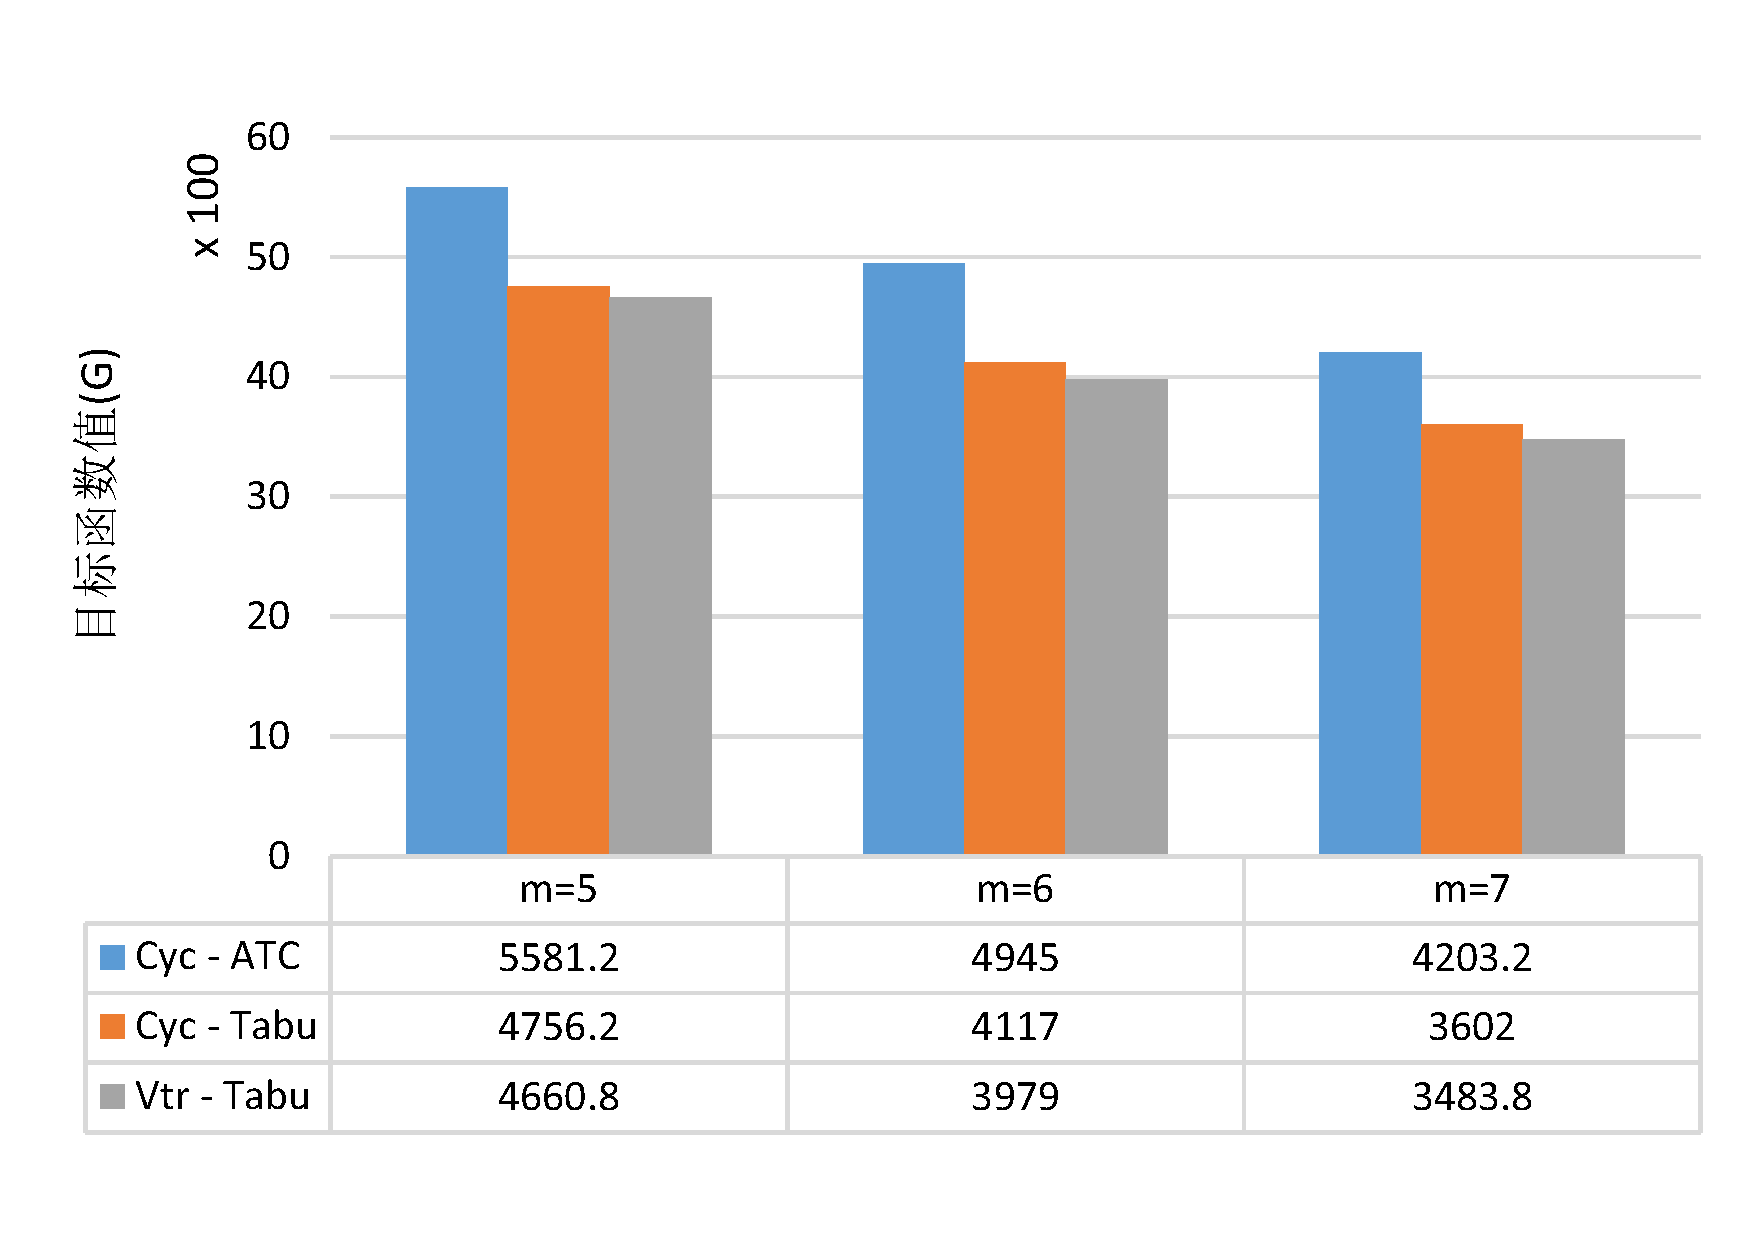
\includegraphics[height = 6cm, angle = -90]{basic_04_20}}
\subfloat[$n = 30$]{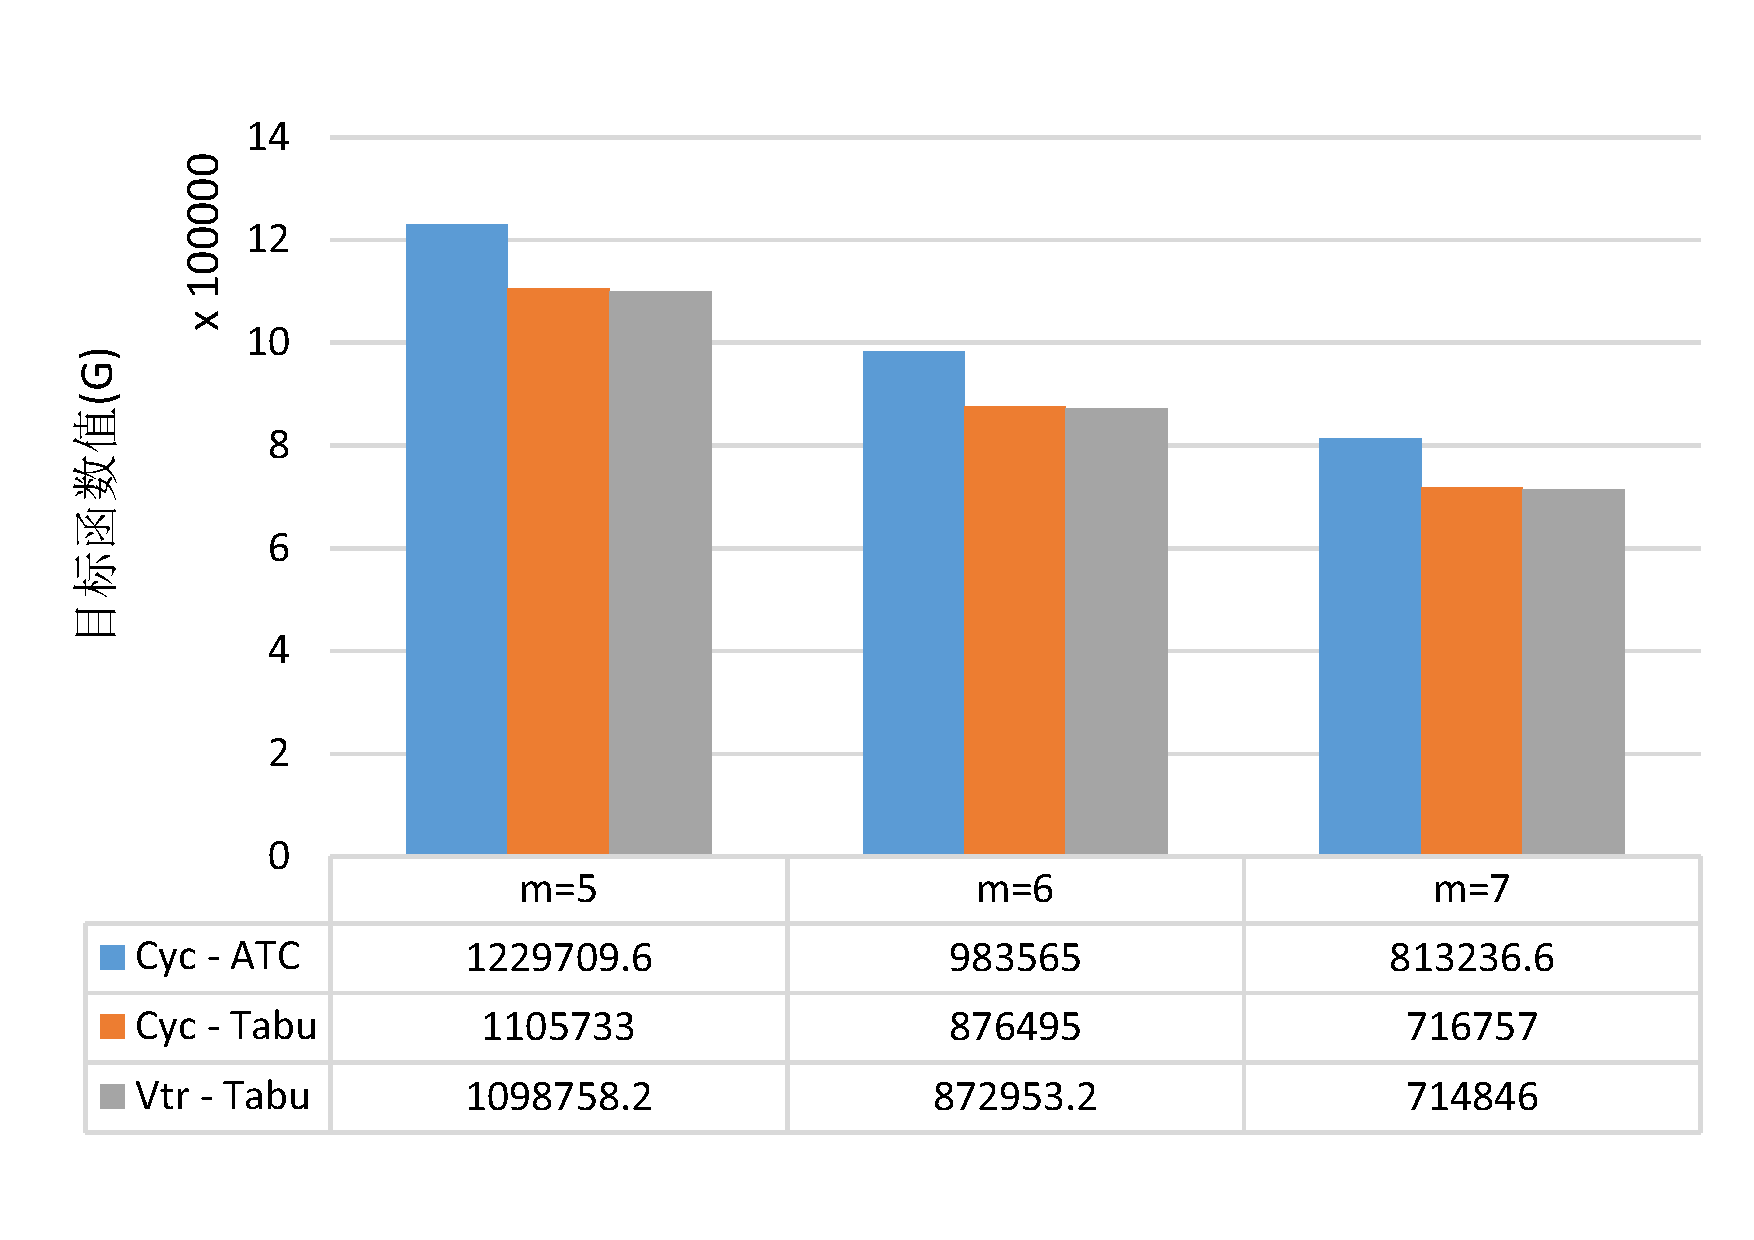
\includegraphics[height = 6cm, angle = -90]{basic_04_300}}
\subfloat[$n = 50$]{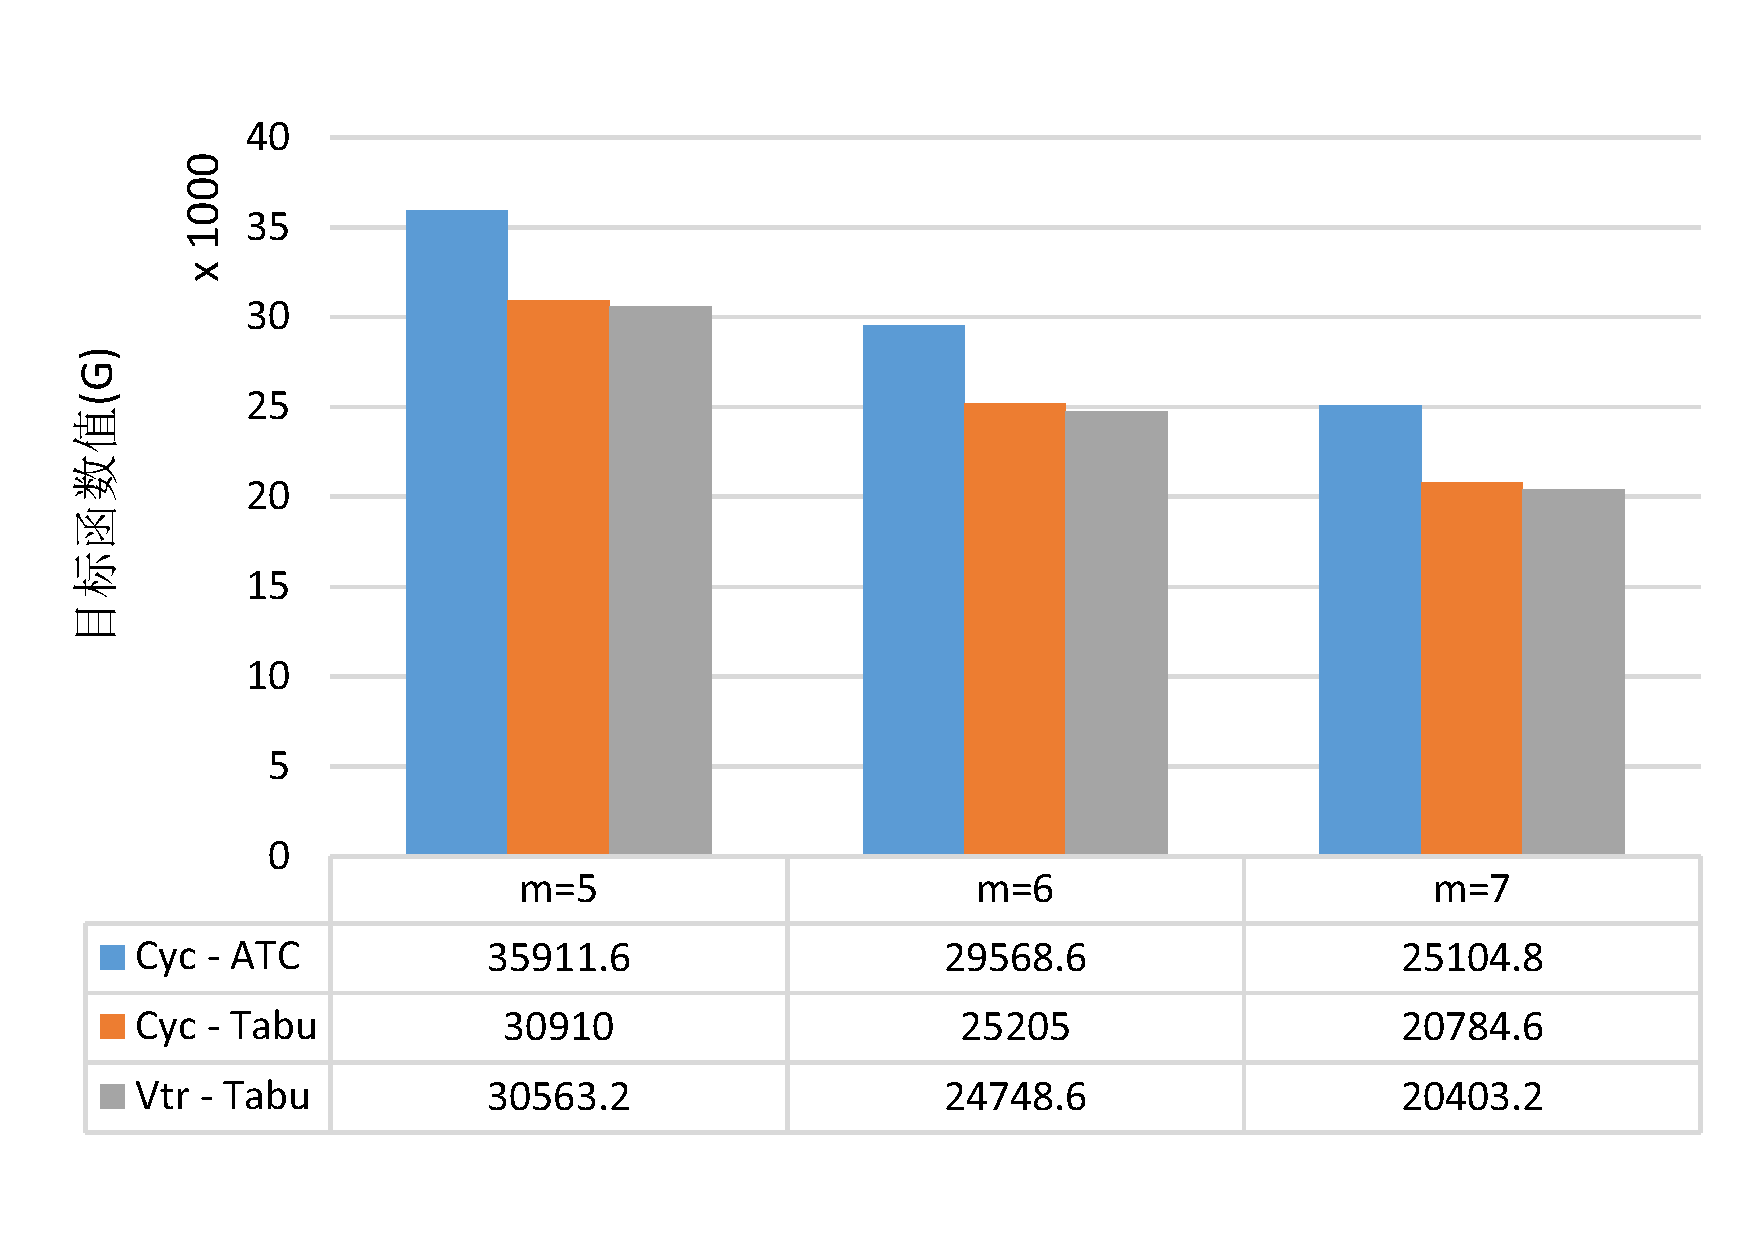
\includegraphics[height = 6cm, angle = -90]{basic_04_50}}
\subfloat[$n = 70$]{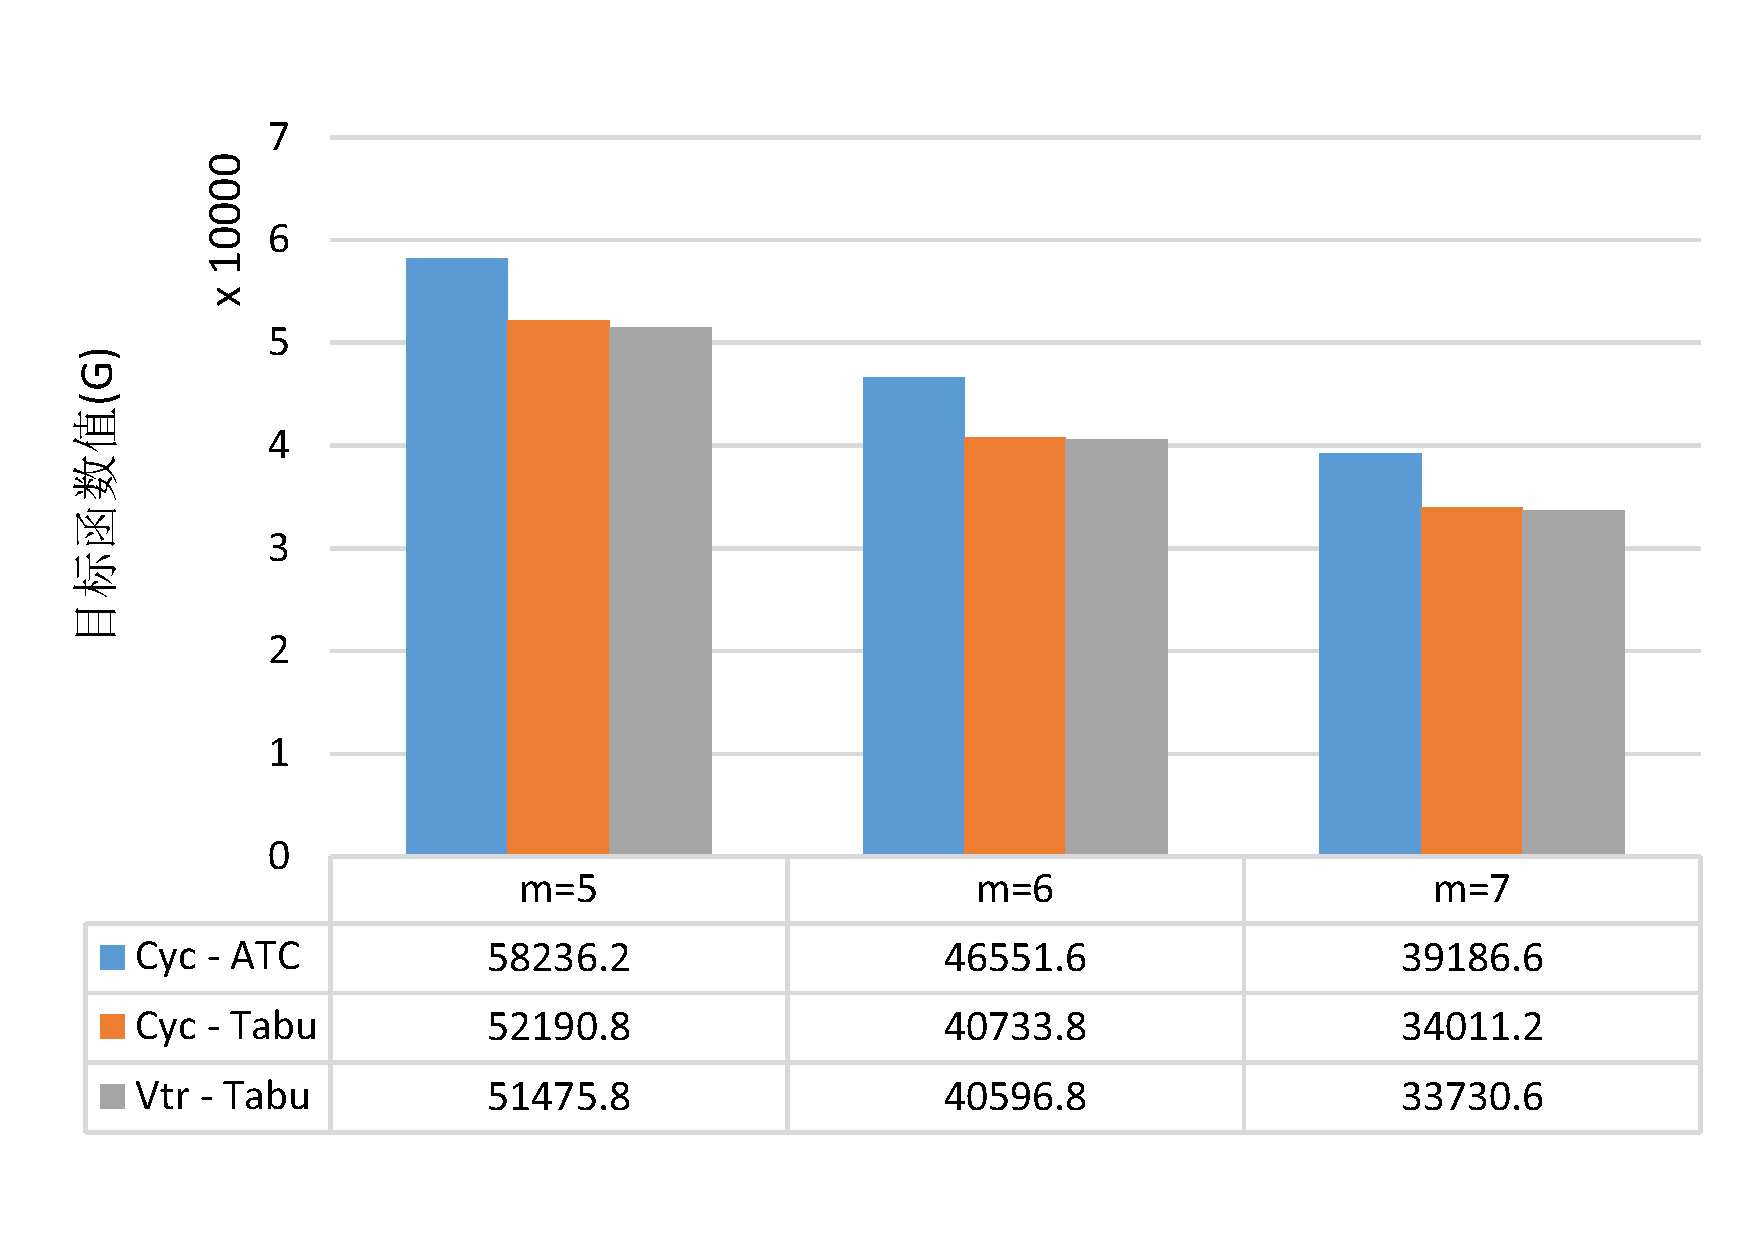
\includegraphics[height = 6cm, angle = -90]{basic_04_70}}\\
\subfloat[$n = 100$]{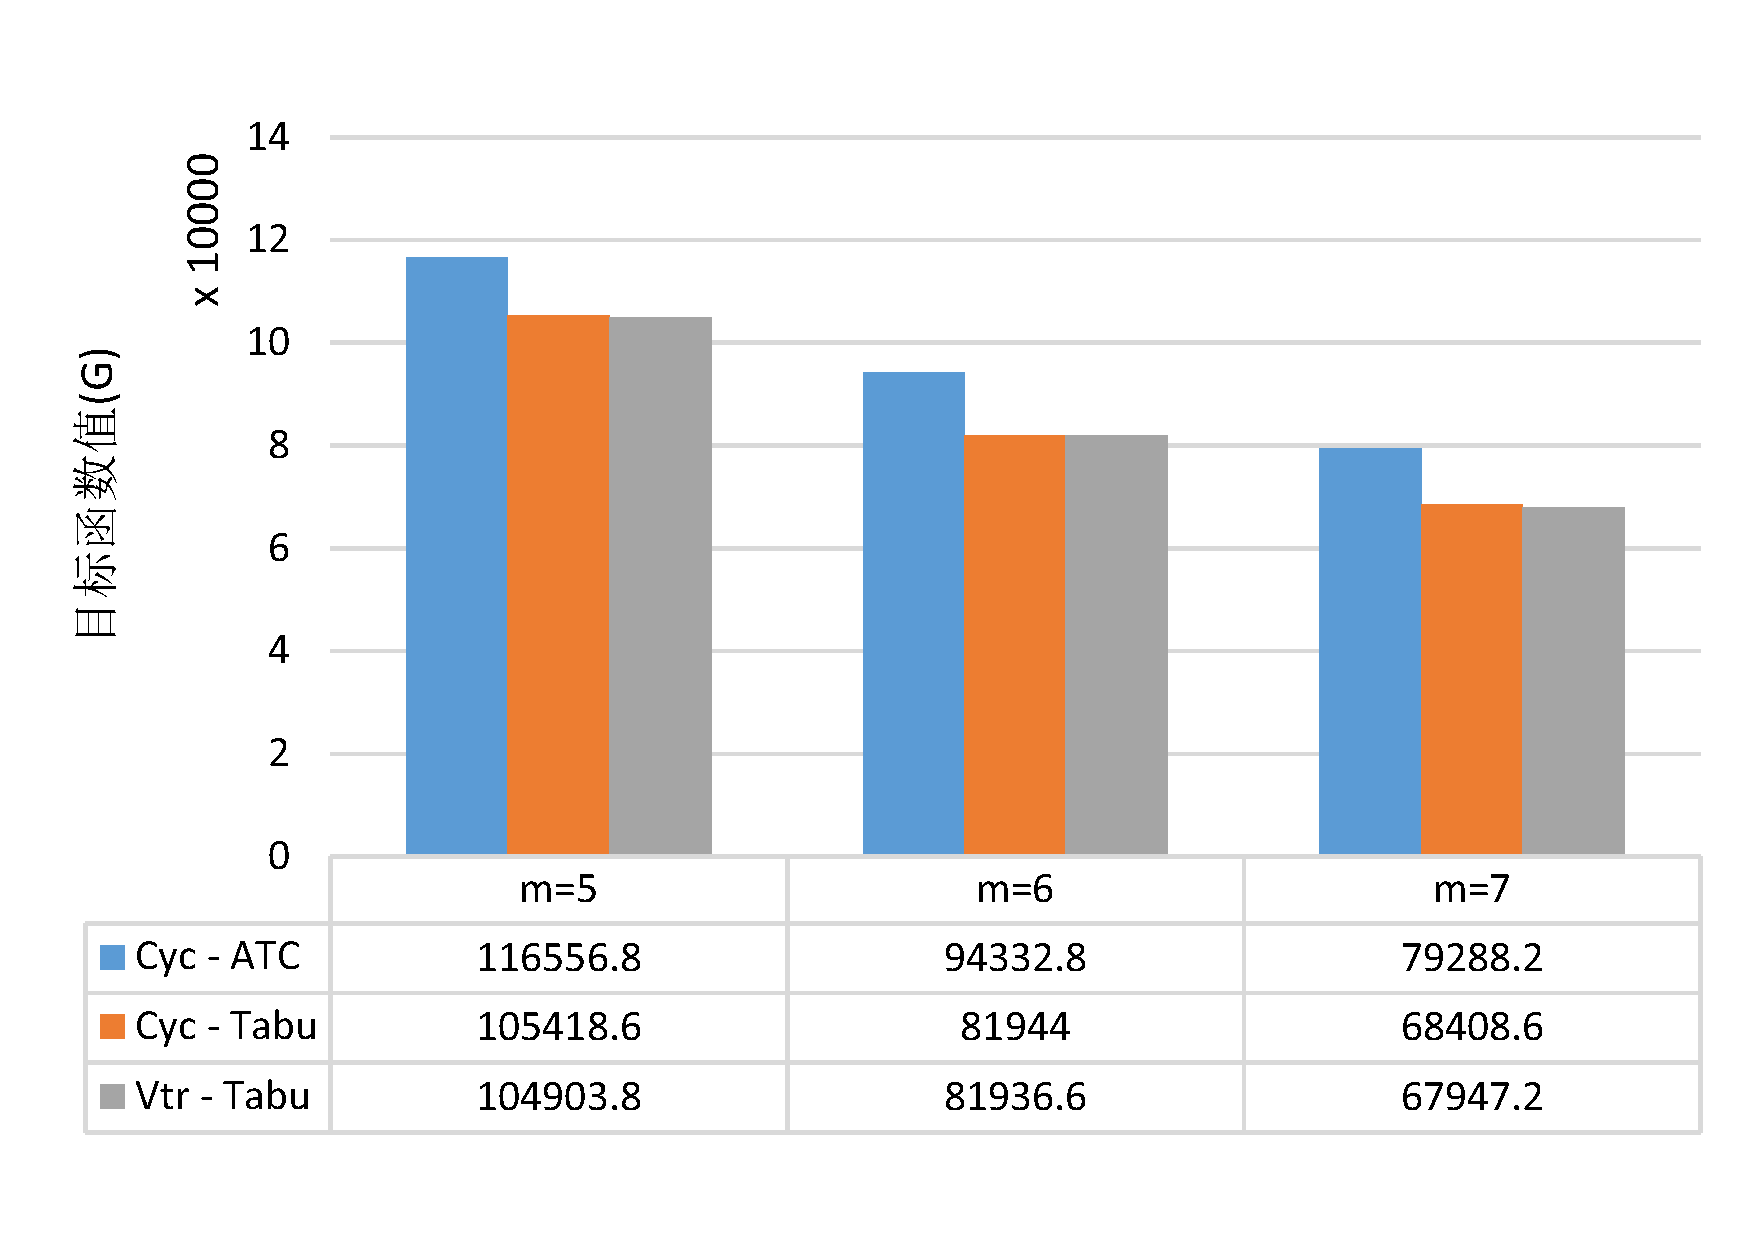
\includegraphics[height = 6cm, angle = -90]{basic_04_100}}
\subfloat[$n = 150$]{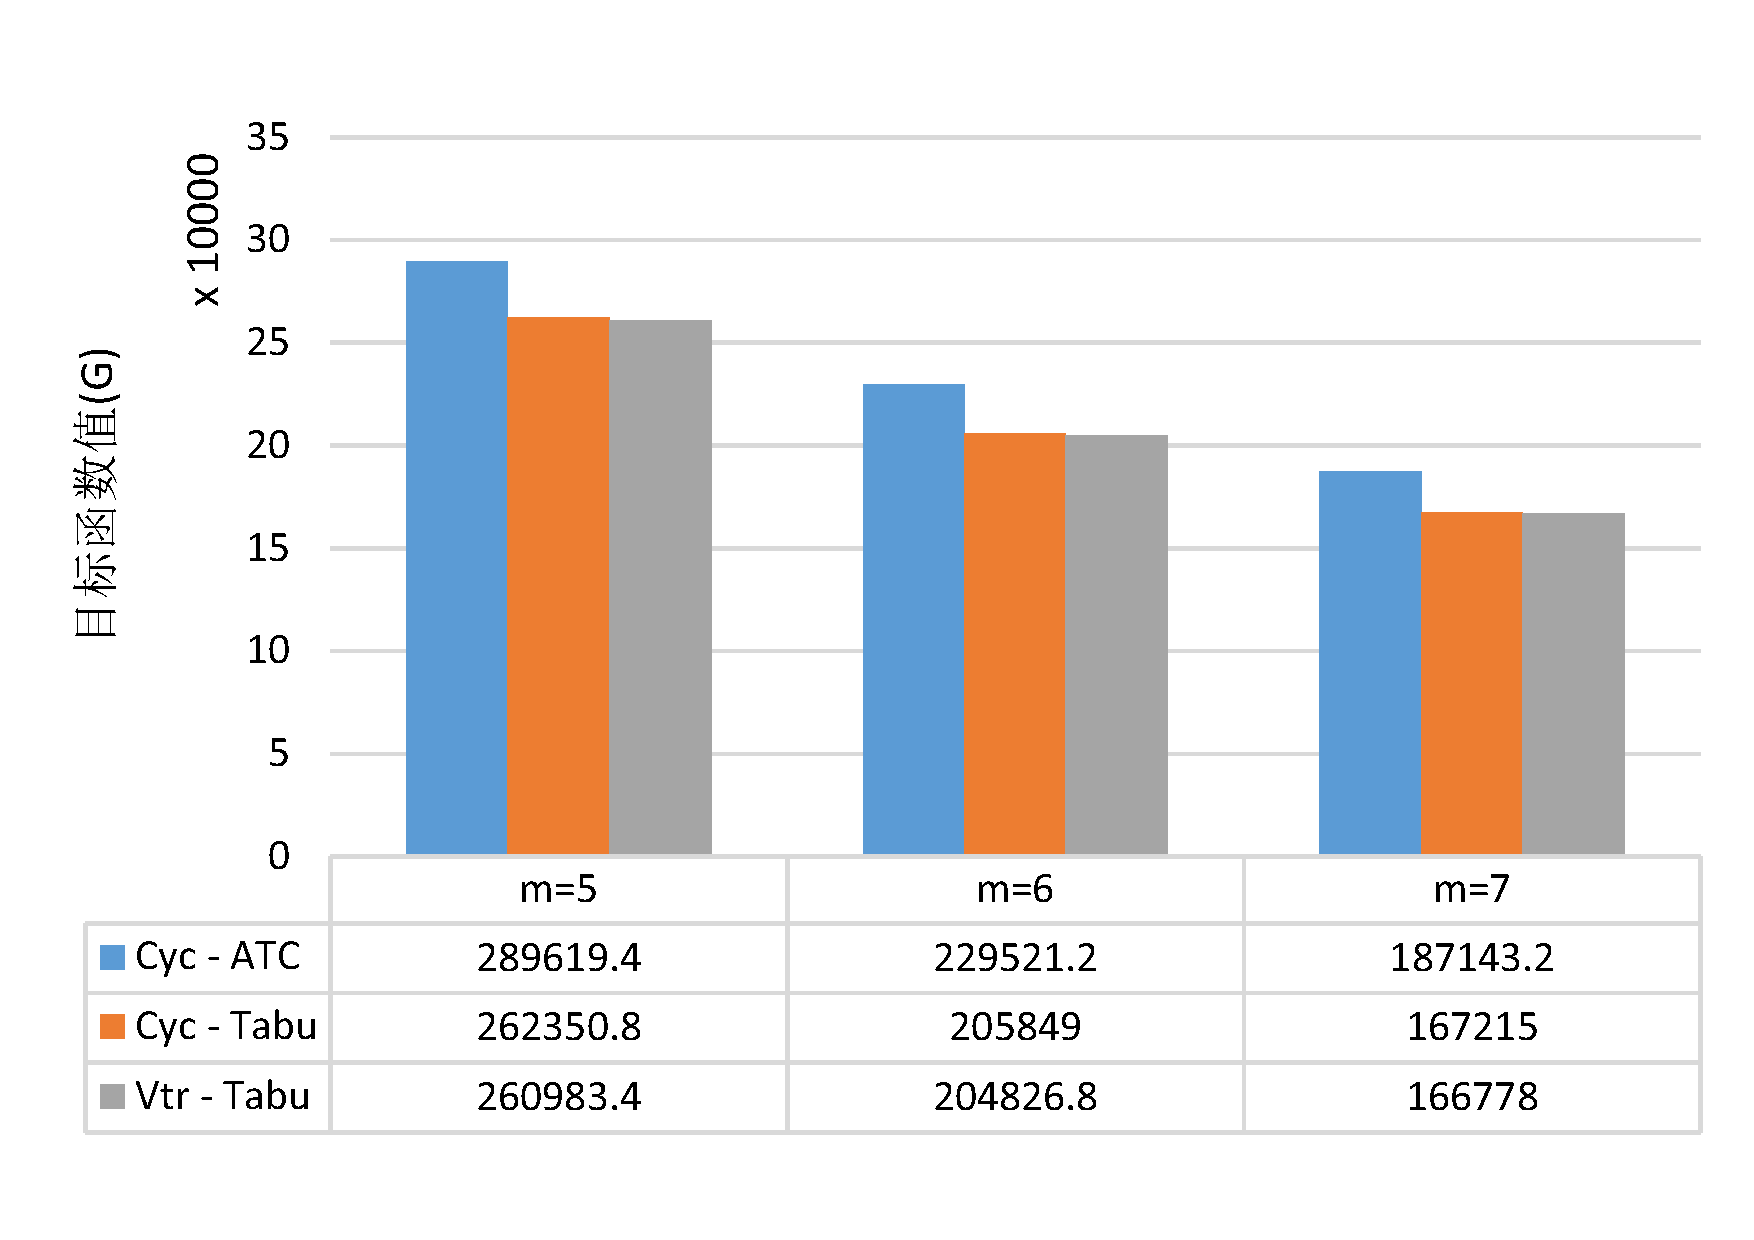
\includegraphics[height = 6cm, angle = -90]{basic_04_150}}
\subfloat[$n = 200$]{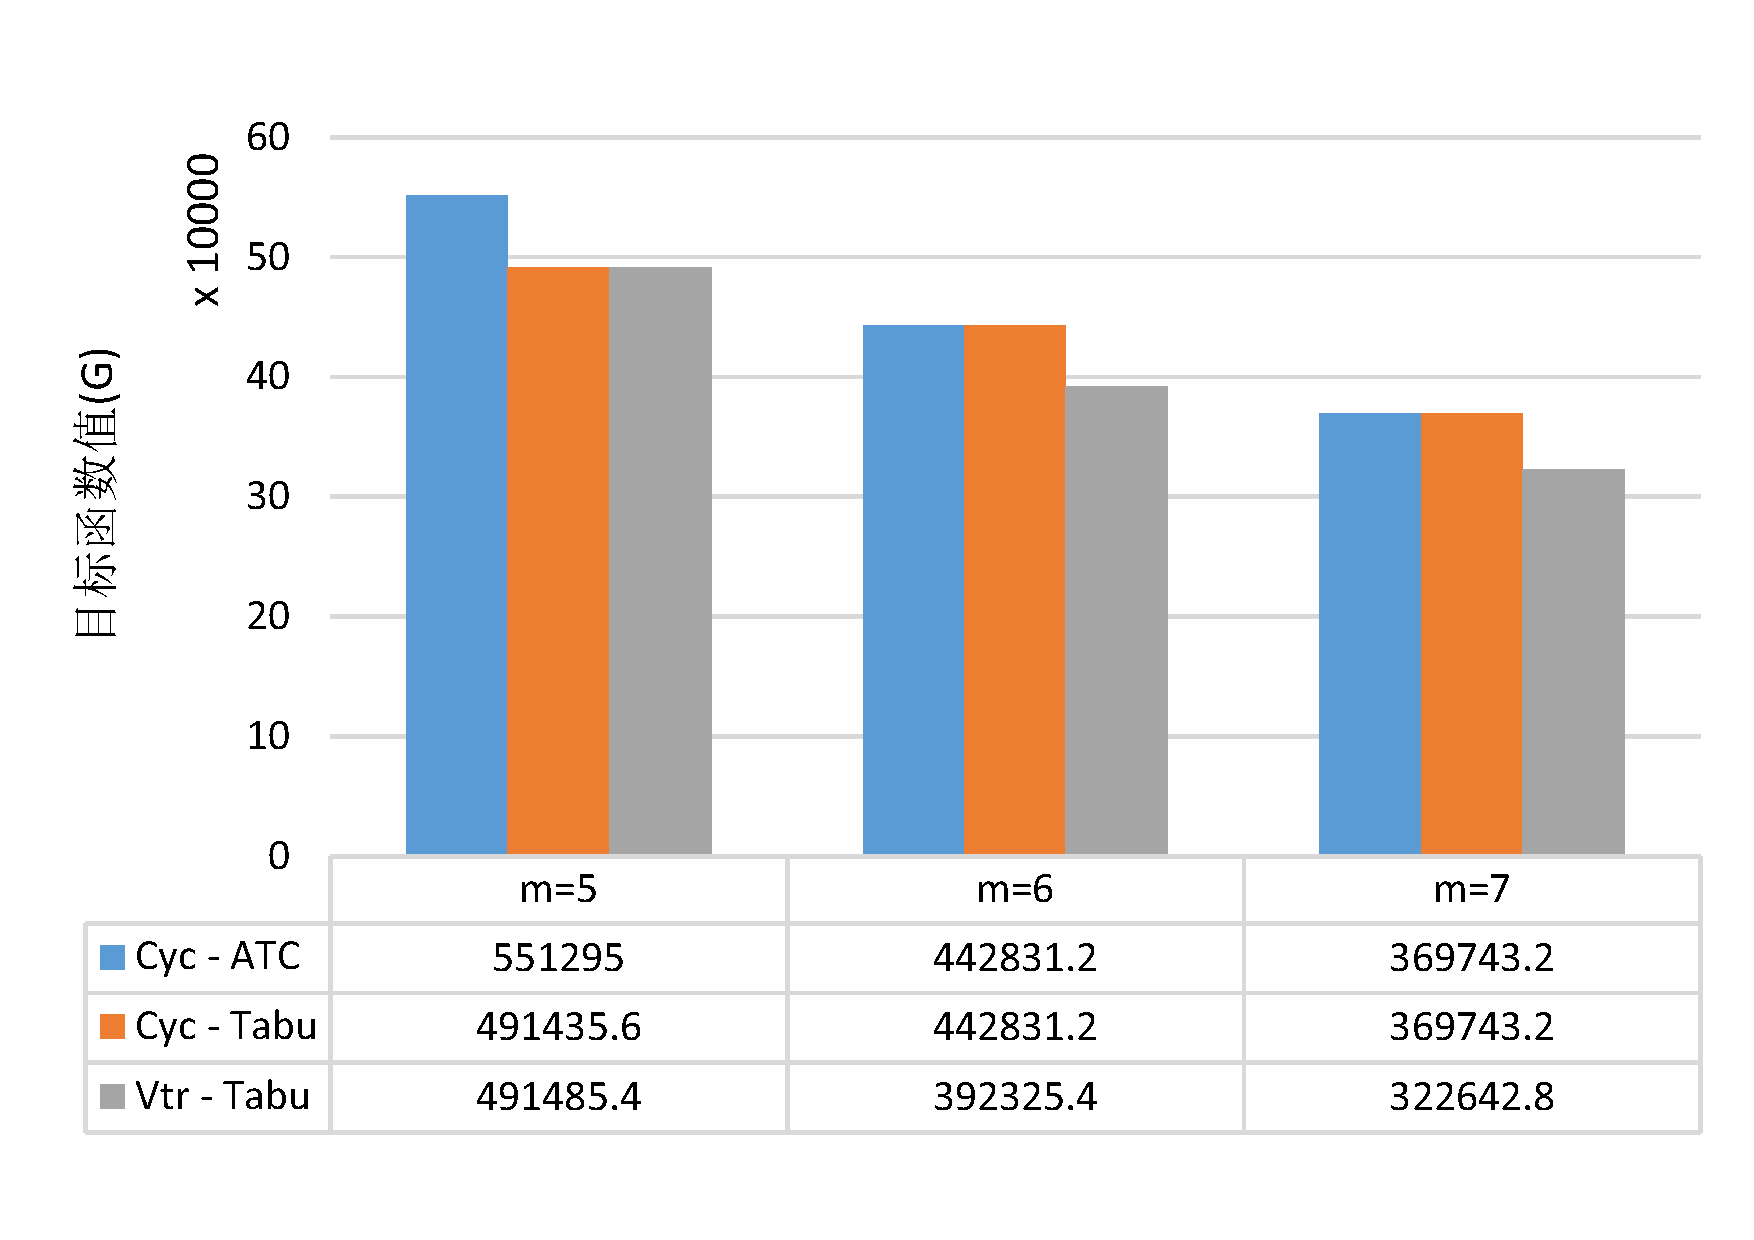
\includegraphics[height = 6cm, angle = -90]{basic_04_200}}
\subfloat[$n = 300$]{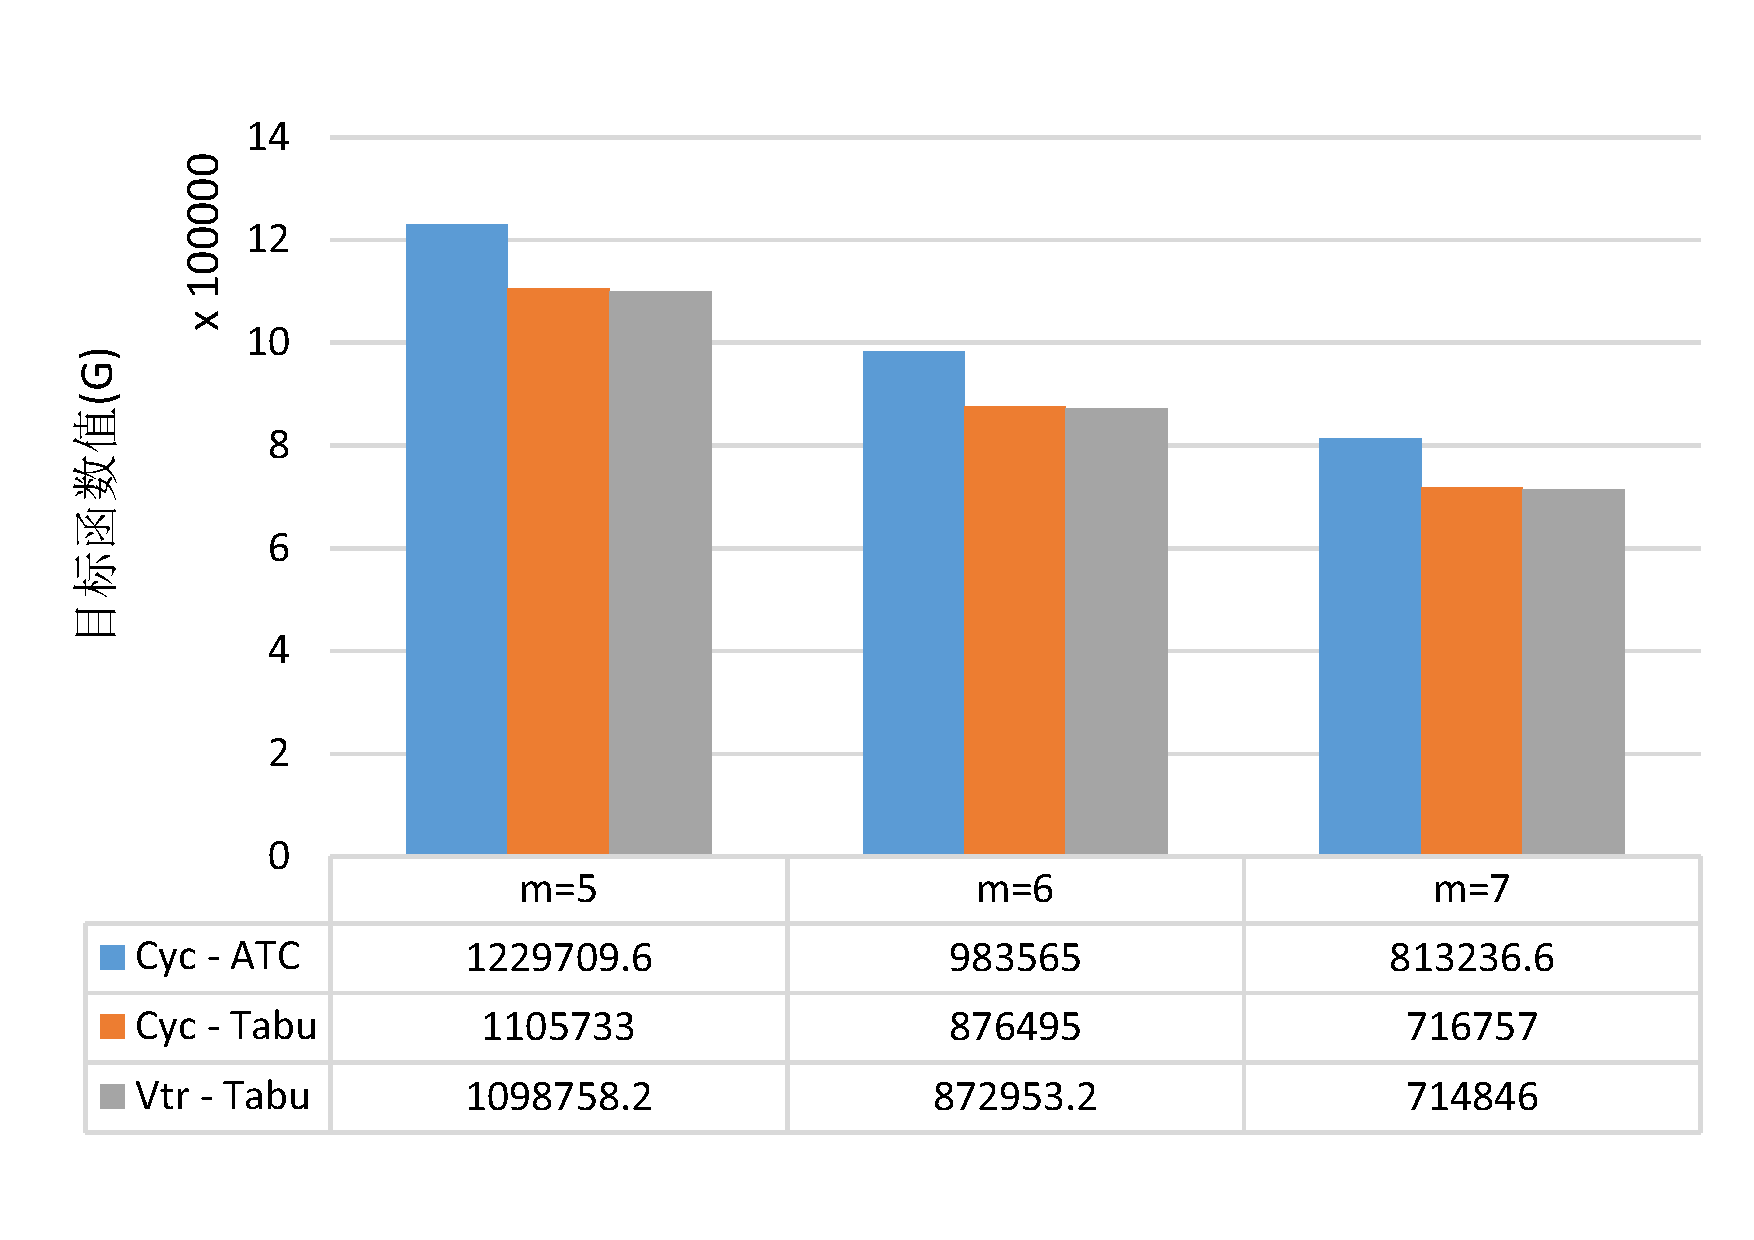
\includegraphics[height = 6cm, angle = -90]{basic_04_300}}\\
\subfloat[$n = 500$]{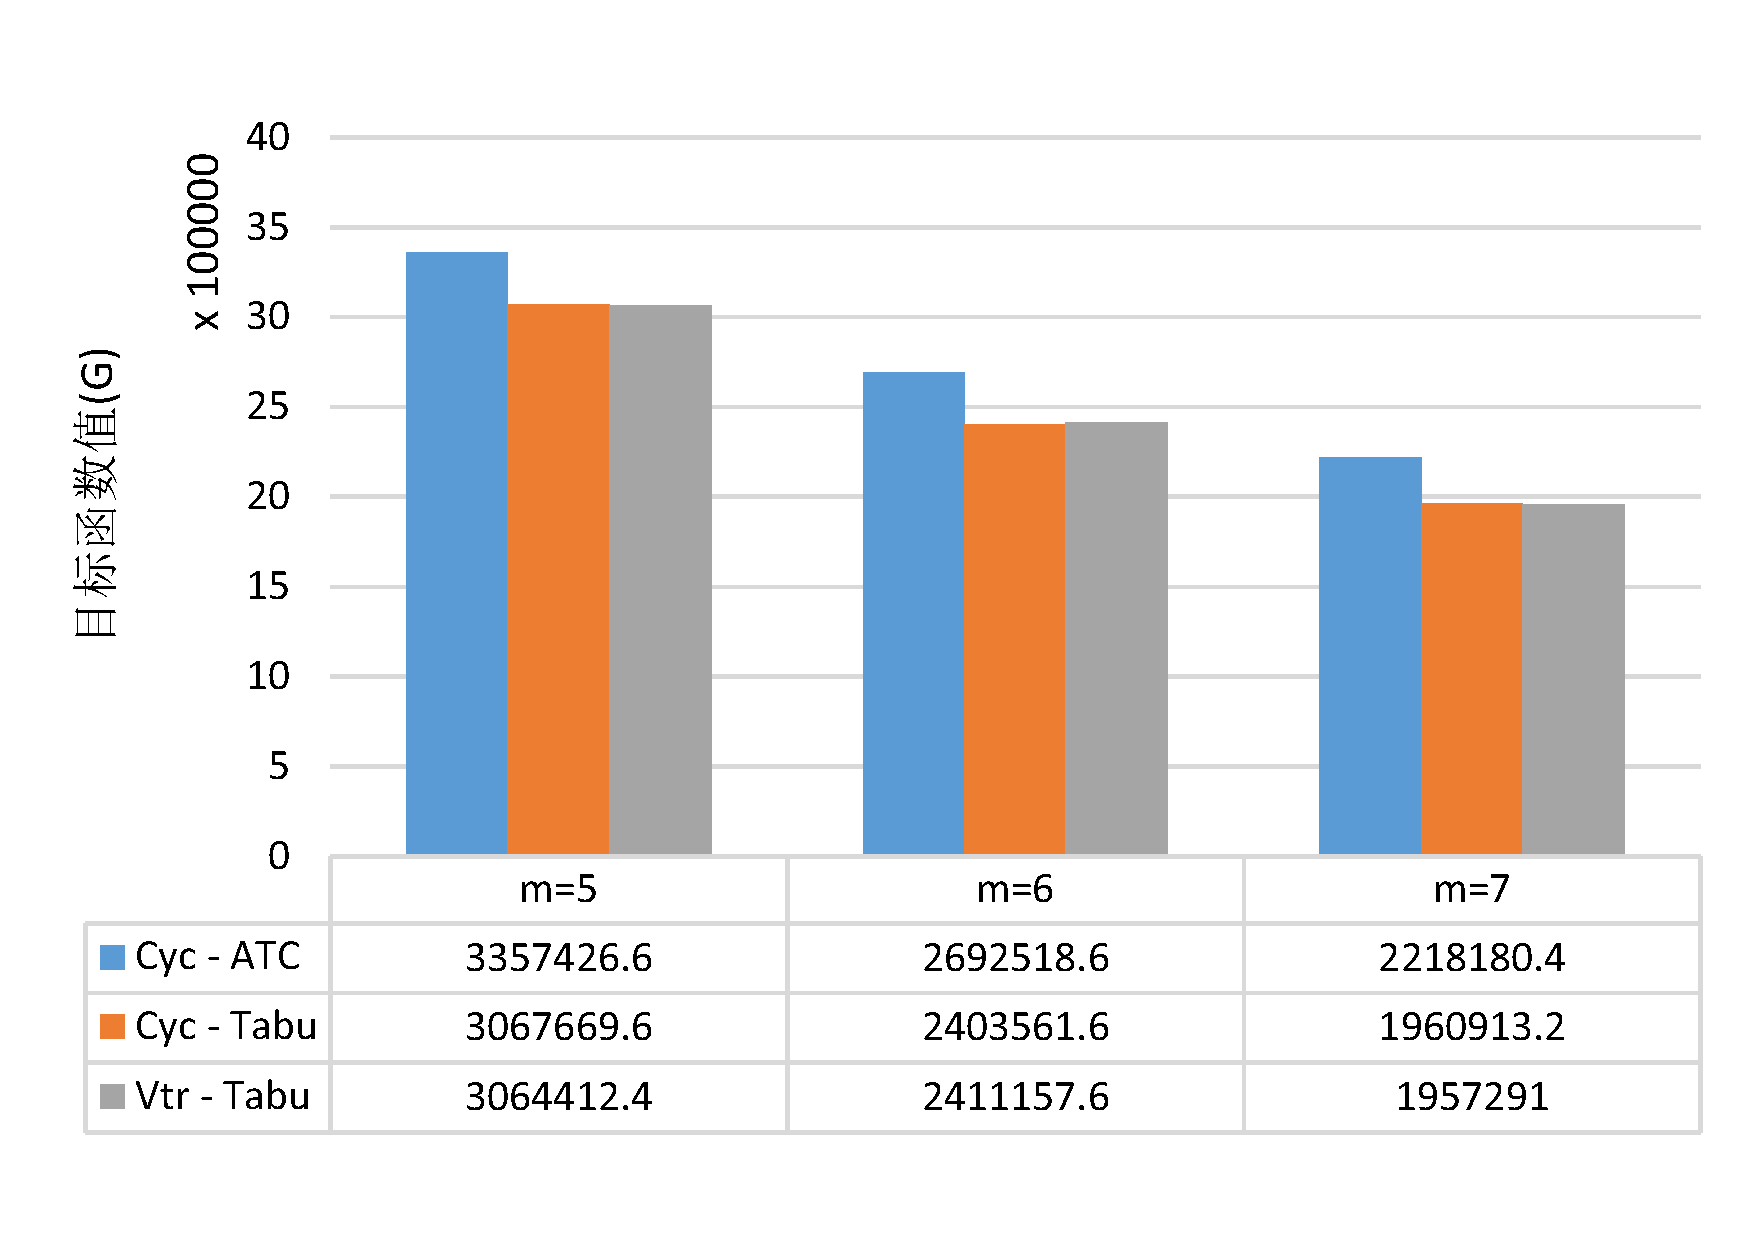
\includegraphics[height = 6cm, angle = -90]{basic_04_500}}
\subfloat[$n = 750$]{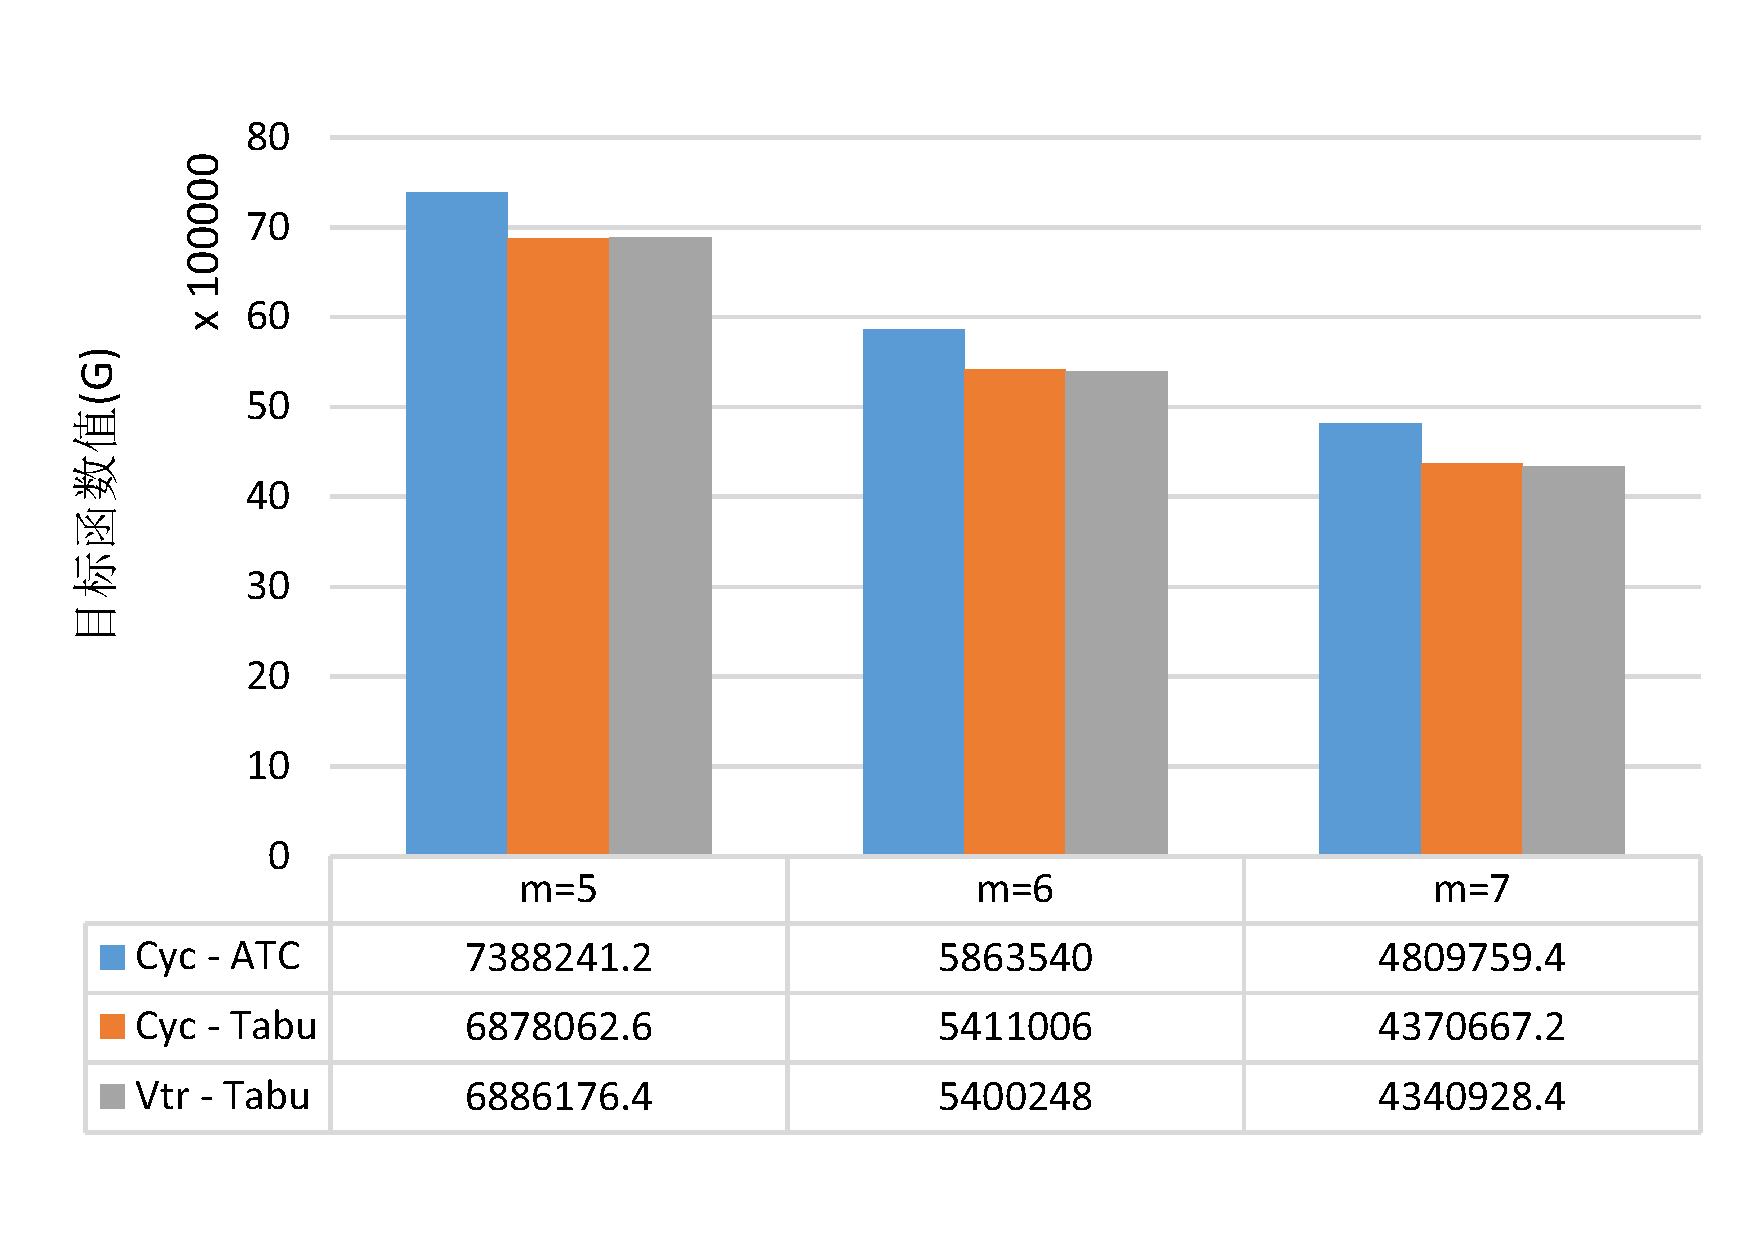
\includegraphics[height = 6cm, angle = -90]{basic_04_750}}
\subfloat[$n = 1000$]{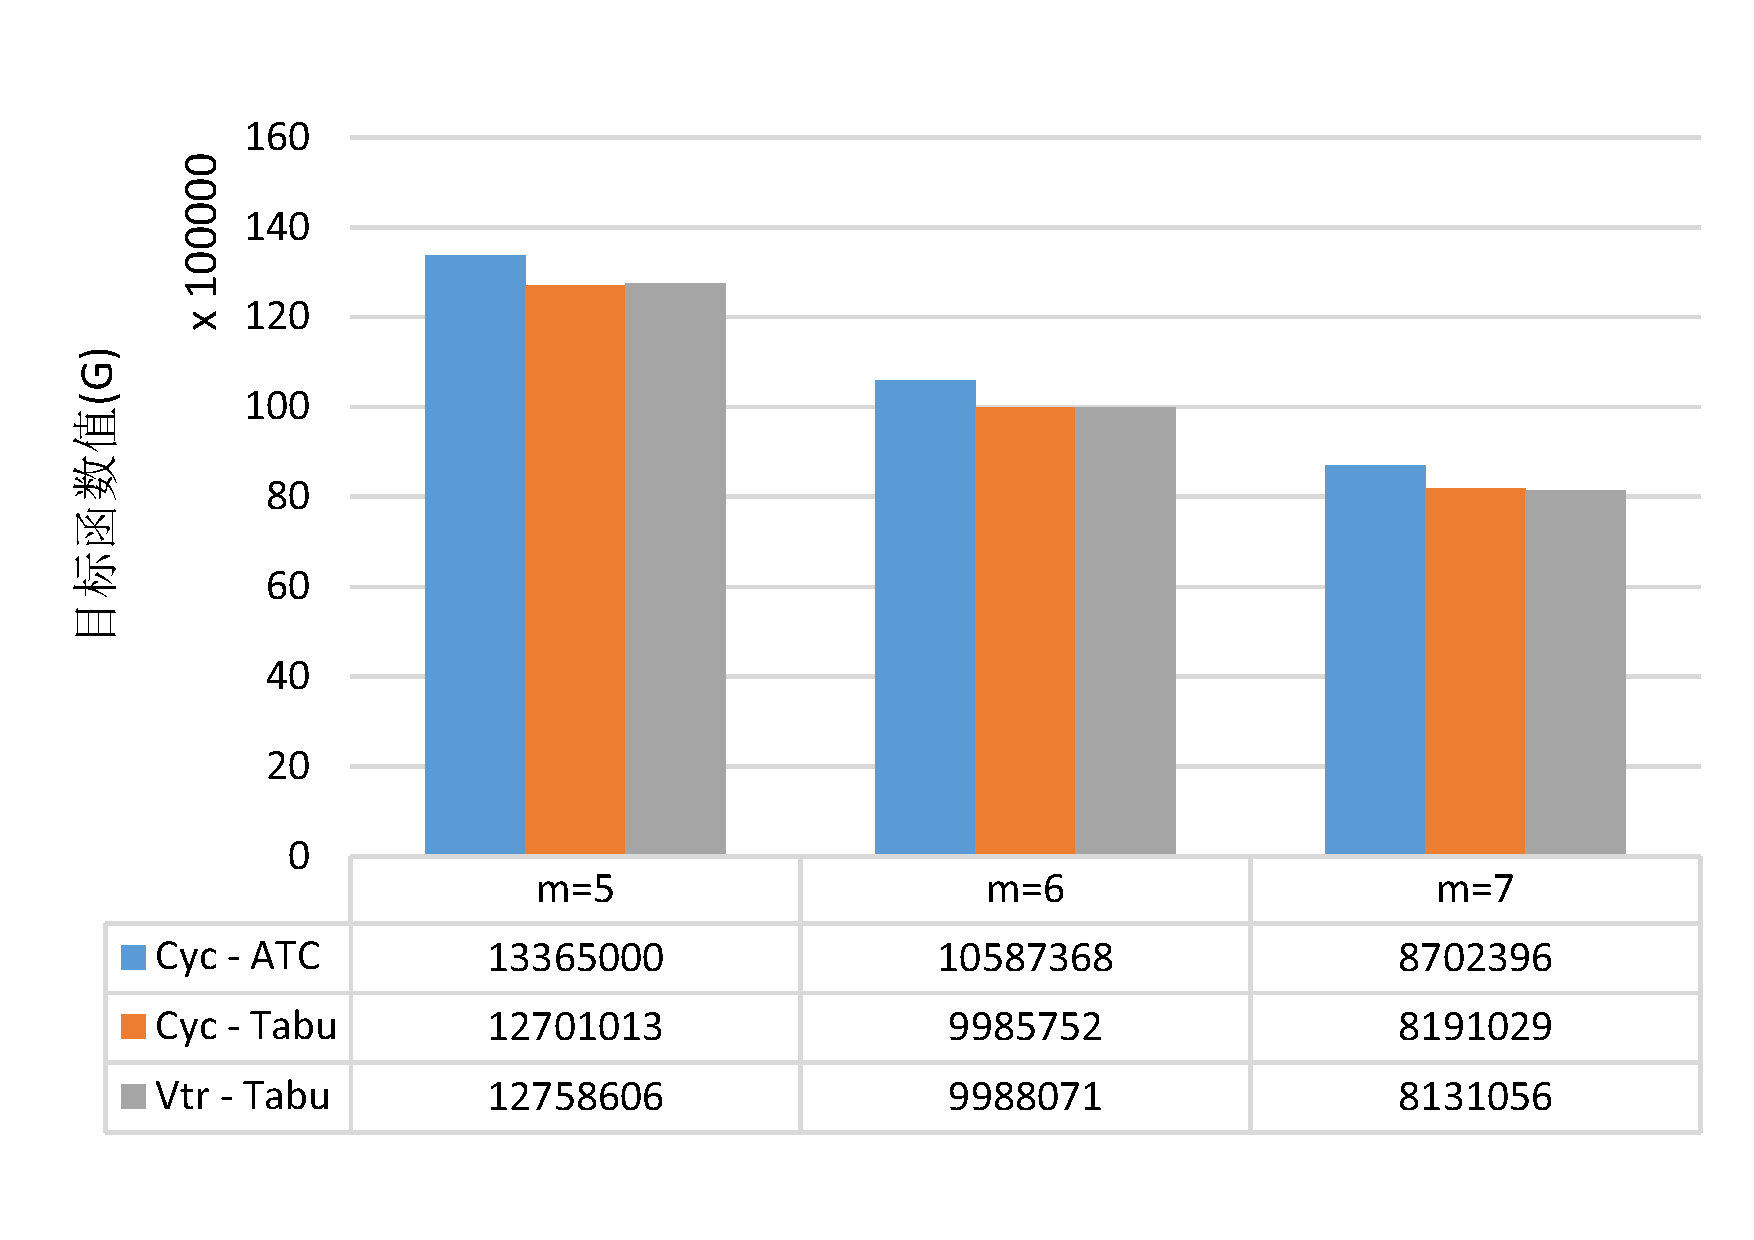
\includegraphics[height = 6cm, angle = -90]{basic_04_1000}}
\caption{\label{fig:result1}模型$1$的Cyc -- ATC、Cyc -- Tabu、Vtr -- Tabu 算法求解目标函数值比较$(\lambda_1 = 0.4)$}
\end{sidewaysfigure}

\begin{sidewaysfigure}
\centering
\subfloat[$n = 20$]{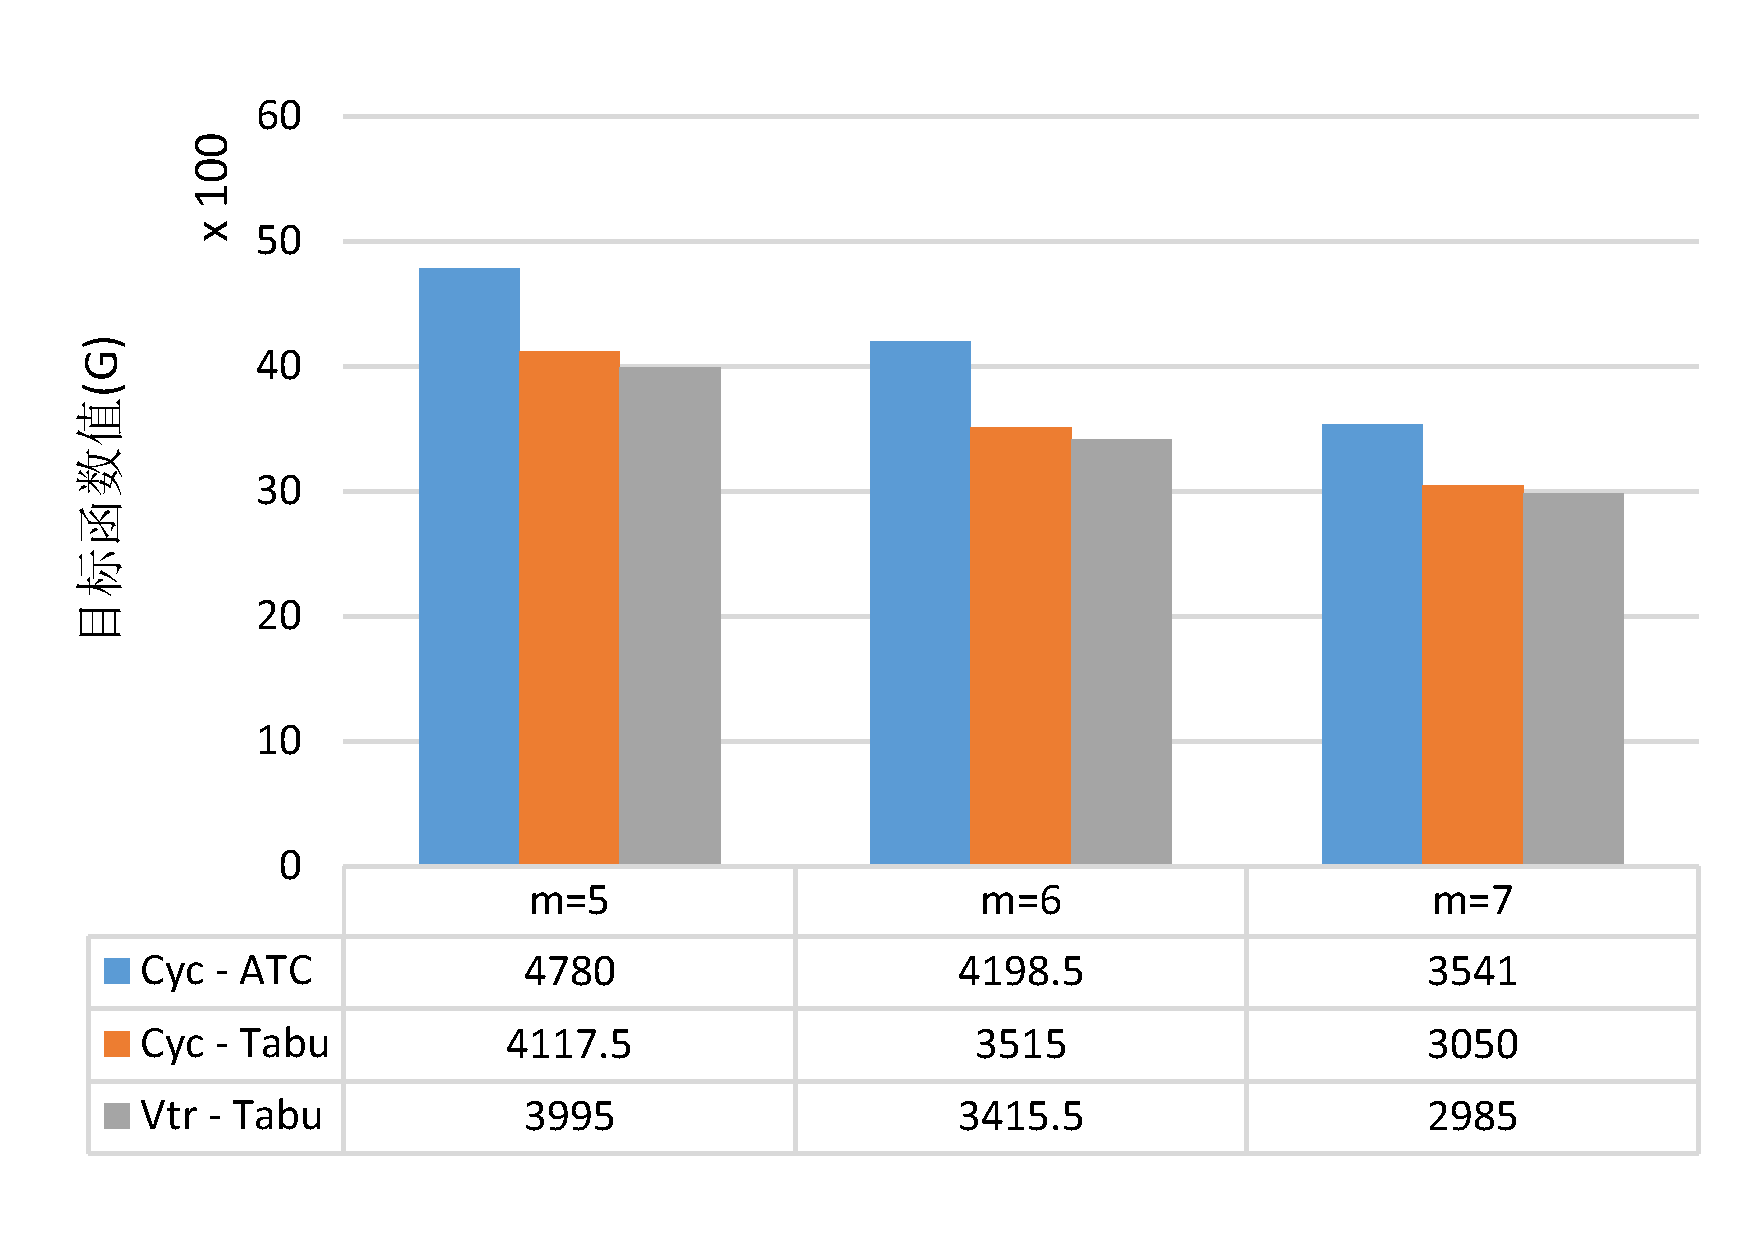
\includegraphics[height = 6cm, angle = -90]{basic_05_20}}
\subfloat[$n = 30$]{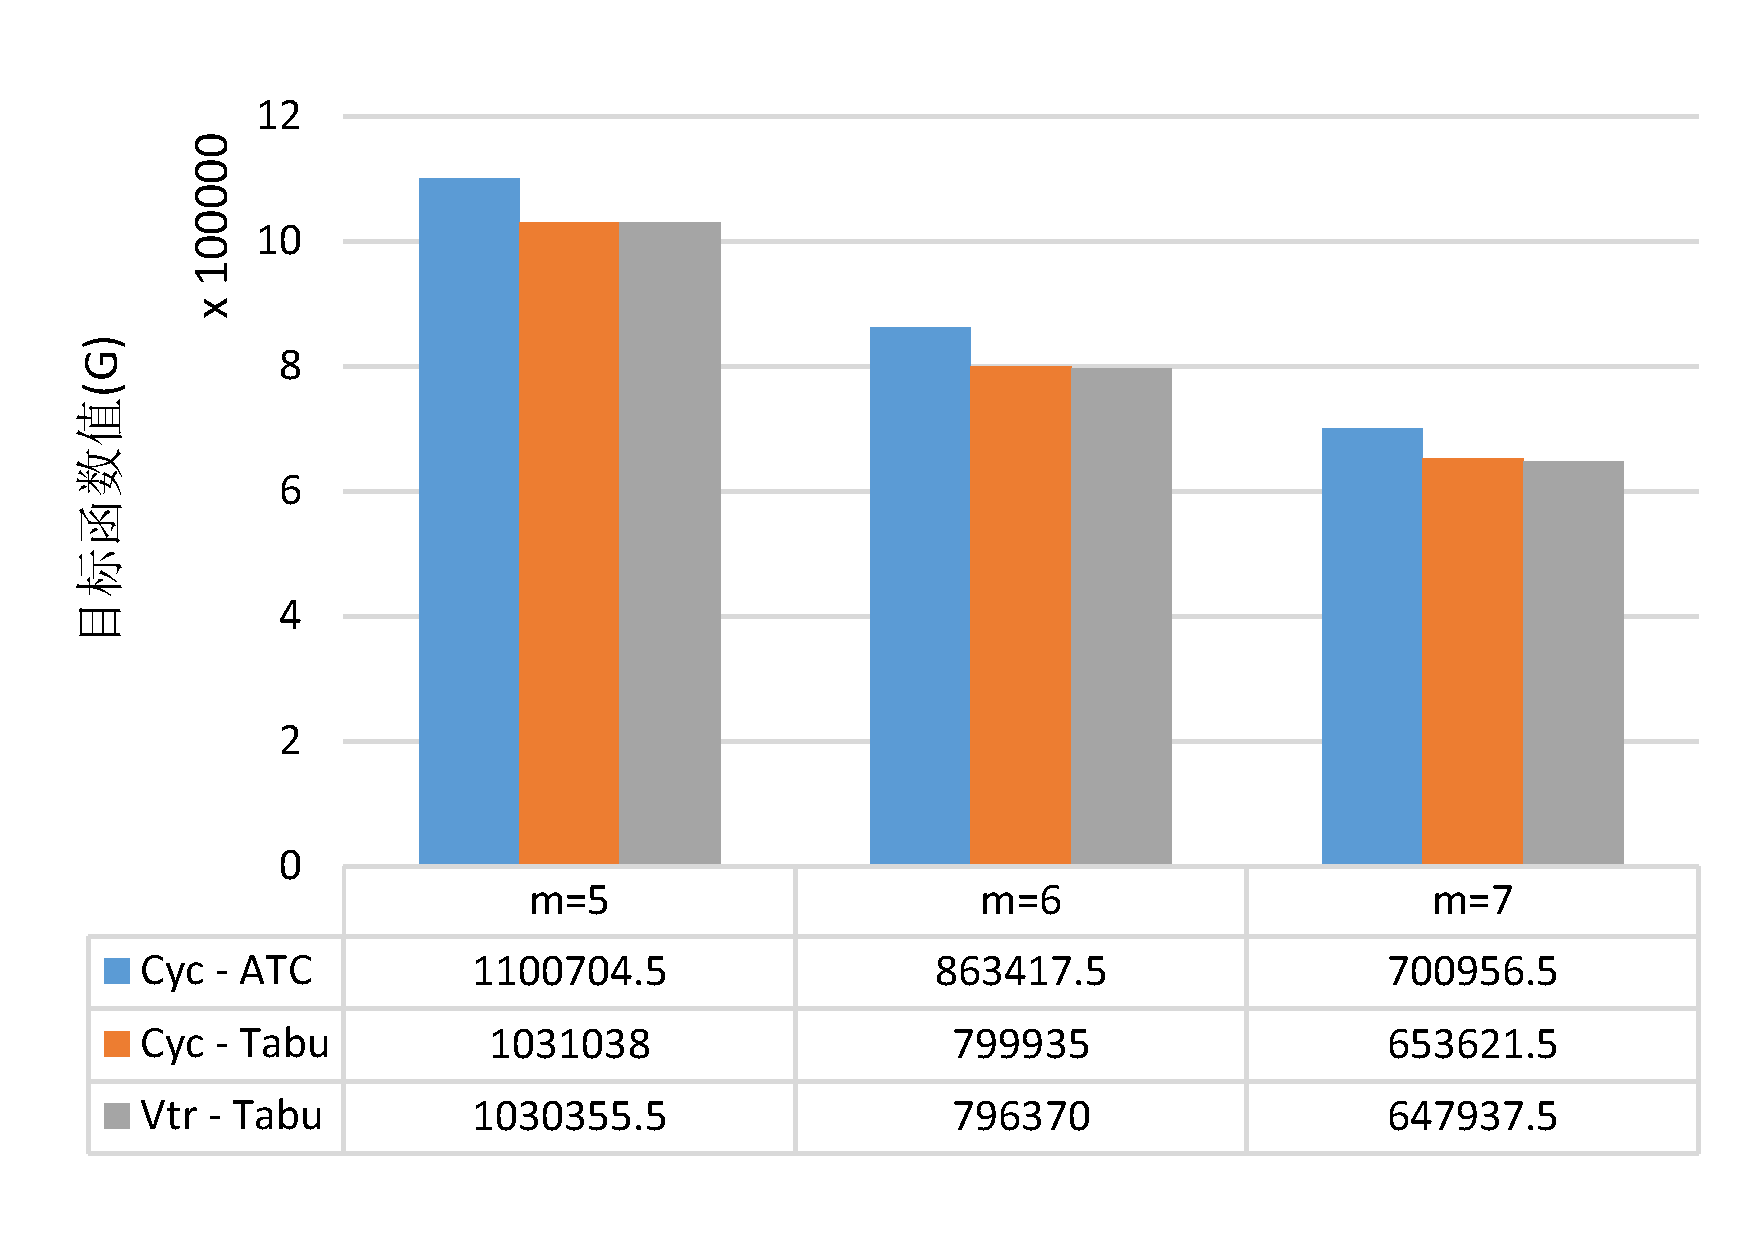
\includegraphics[height = 6cm, angle = -90]{basic_05_300}}
\subfloat[$n = 50$]{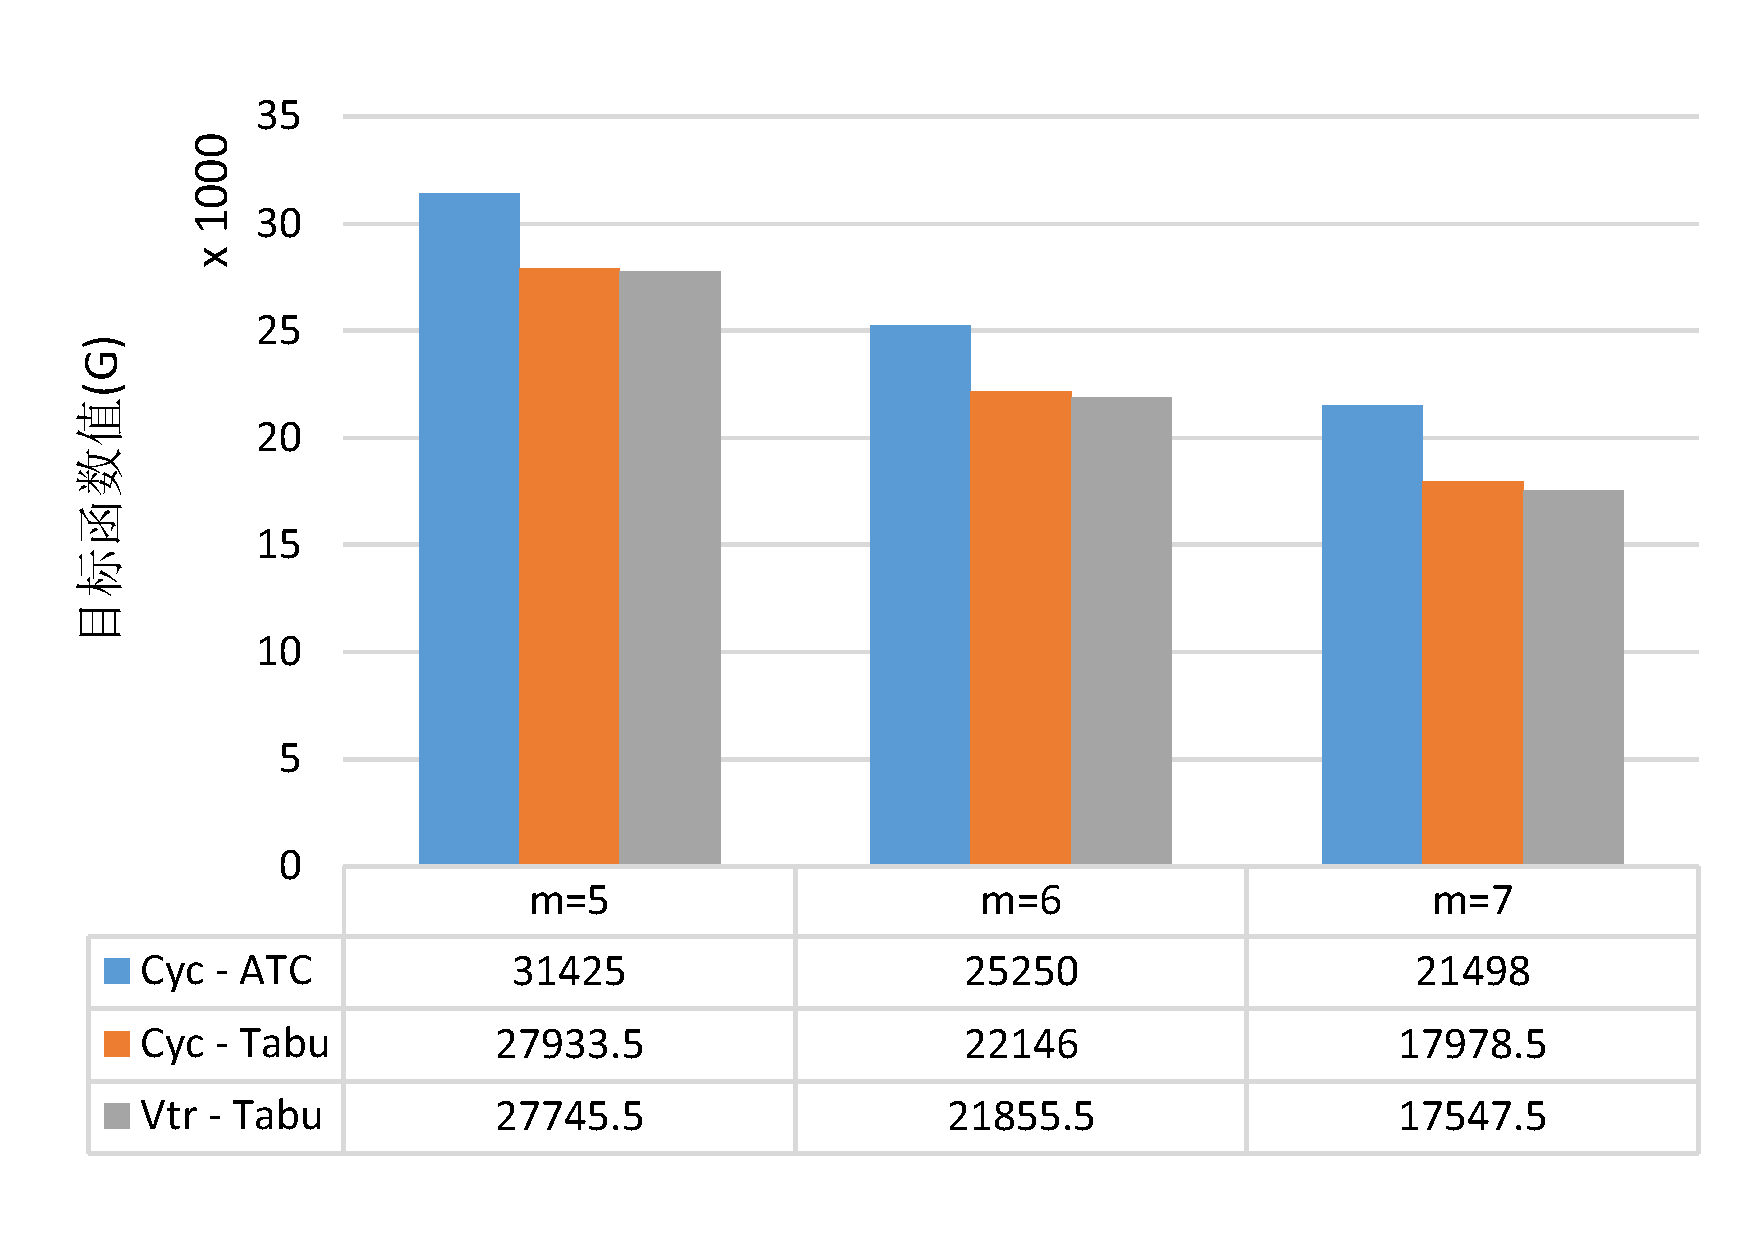
\includegraphics[height = 6cm, angle = -90]{basic_05_50}}
\subfloat[$n = 70$]{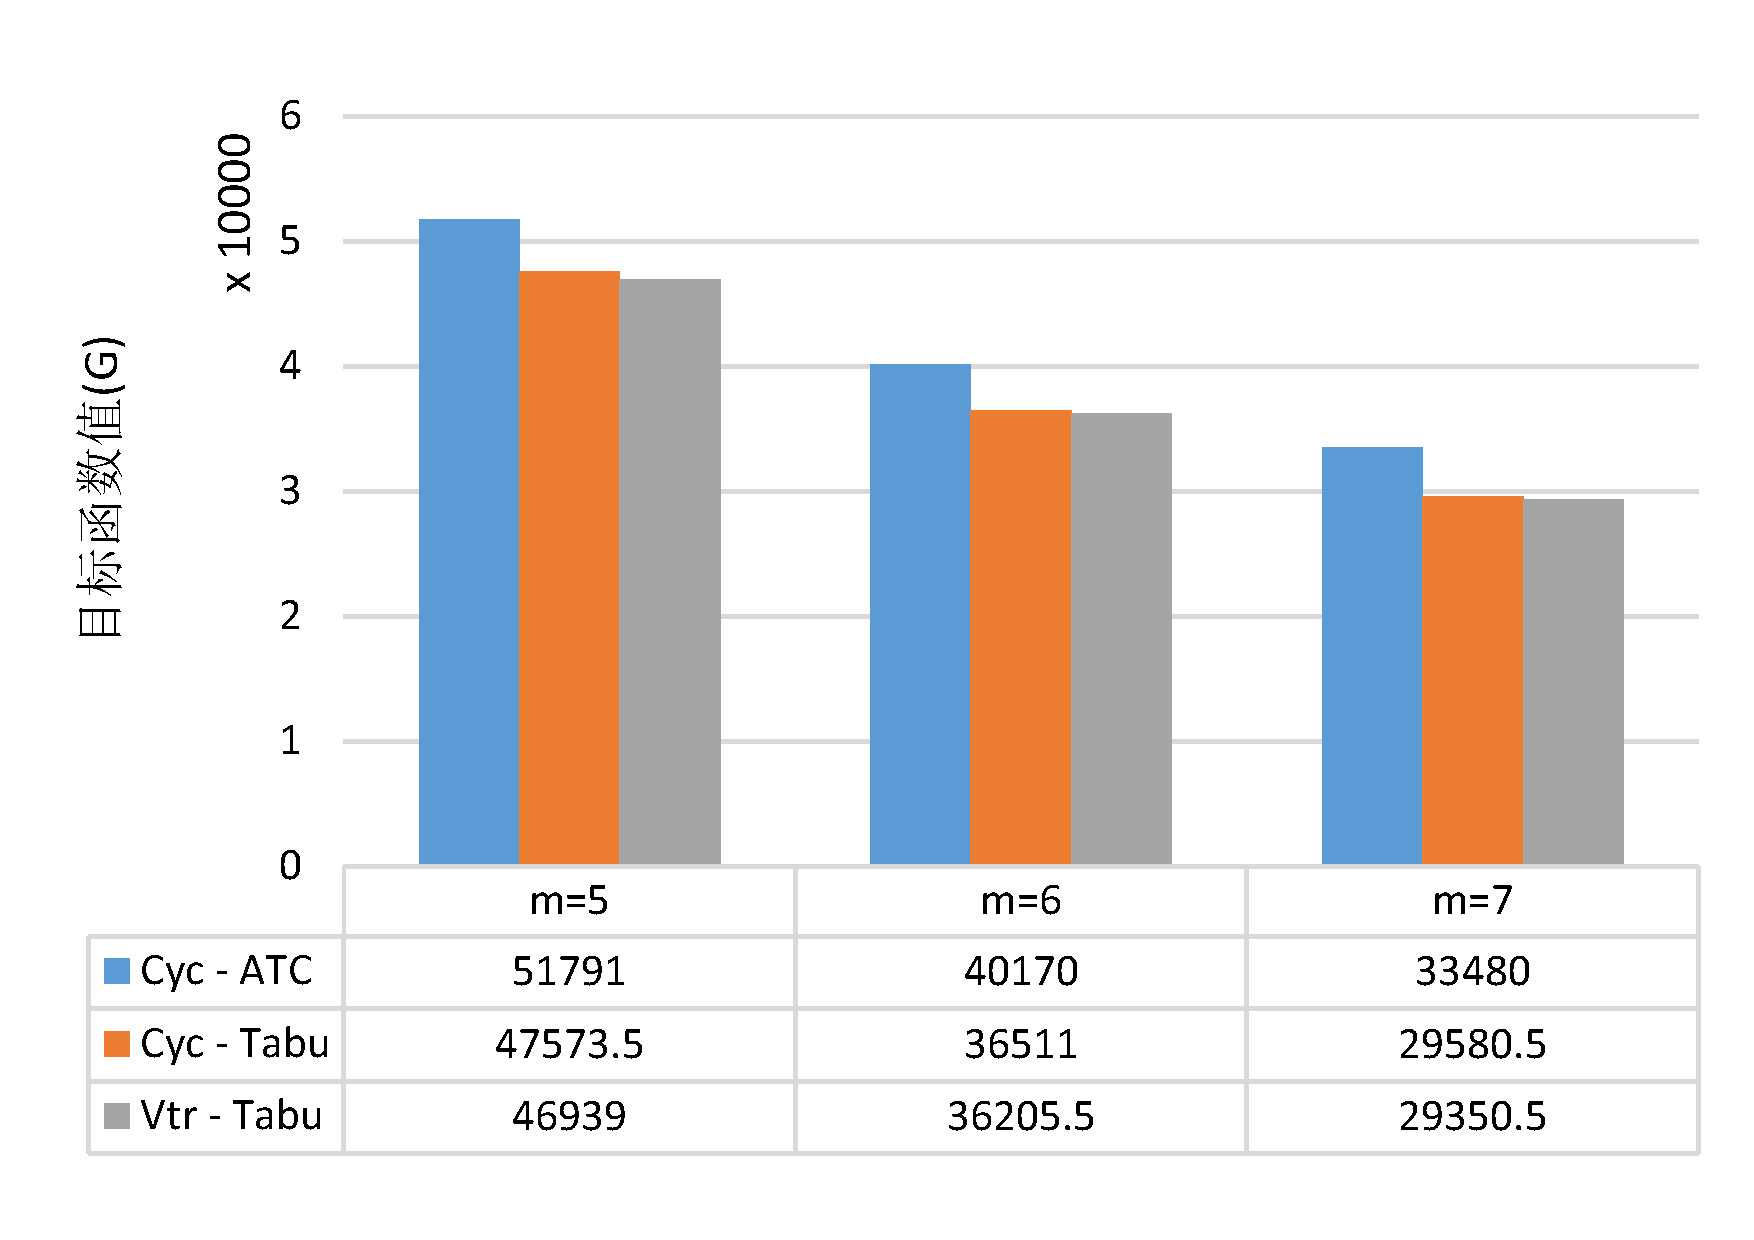
\includegraphics[height = 6cm, angle = -90]{basic_05_70}}\\
\subfloat[$n = 100$]{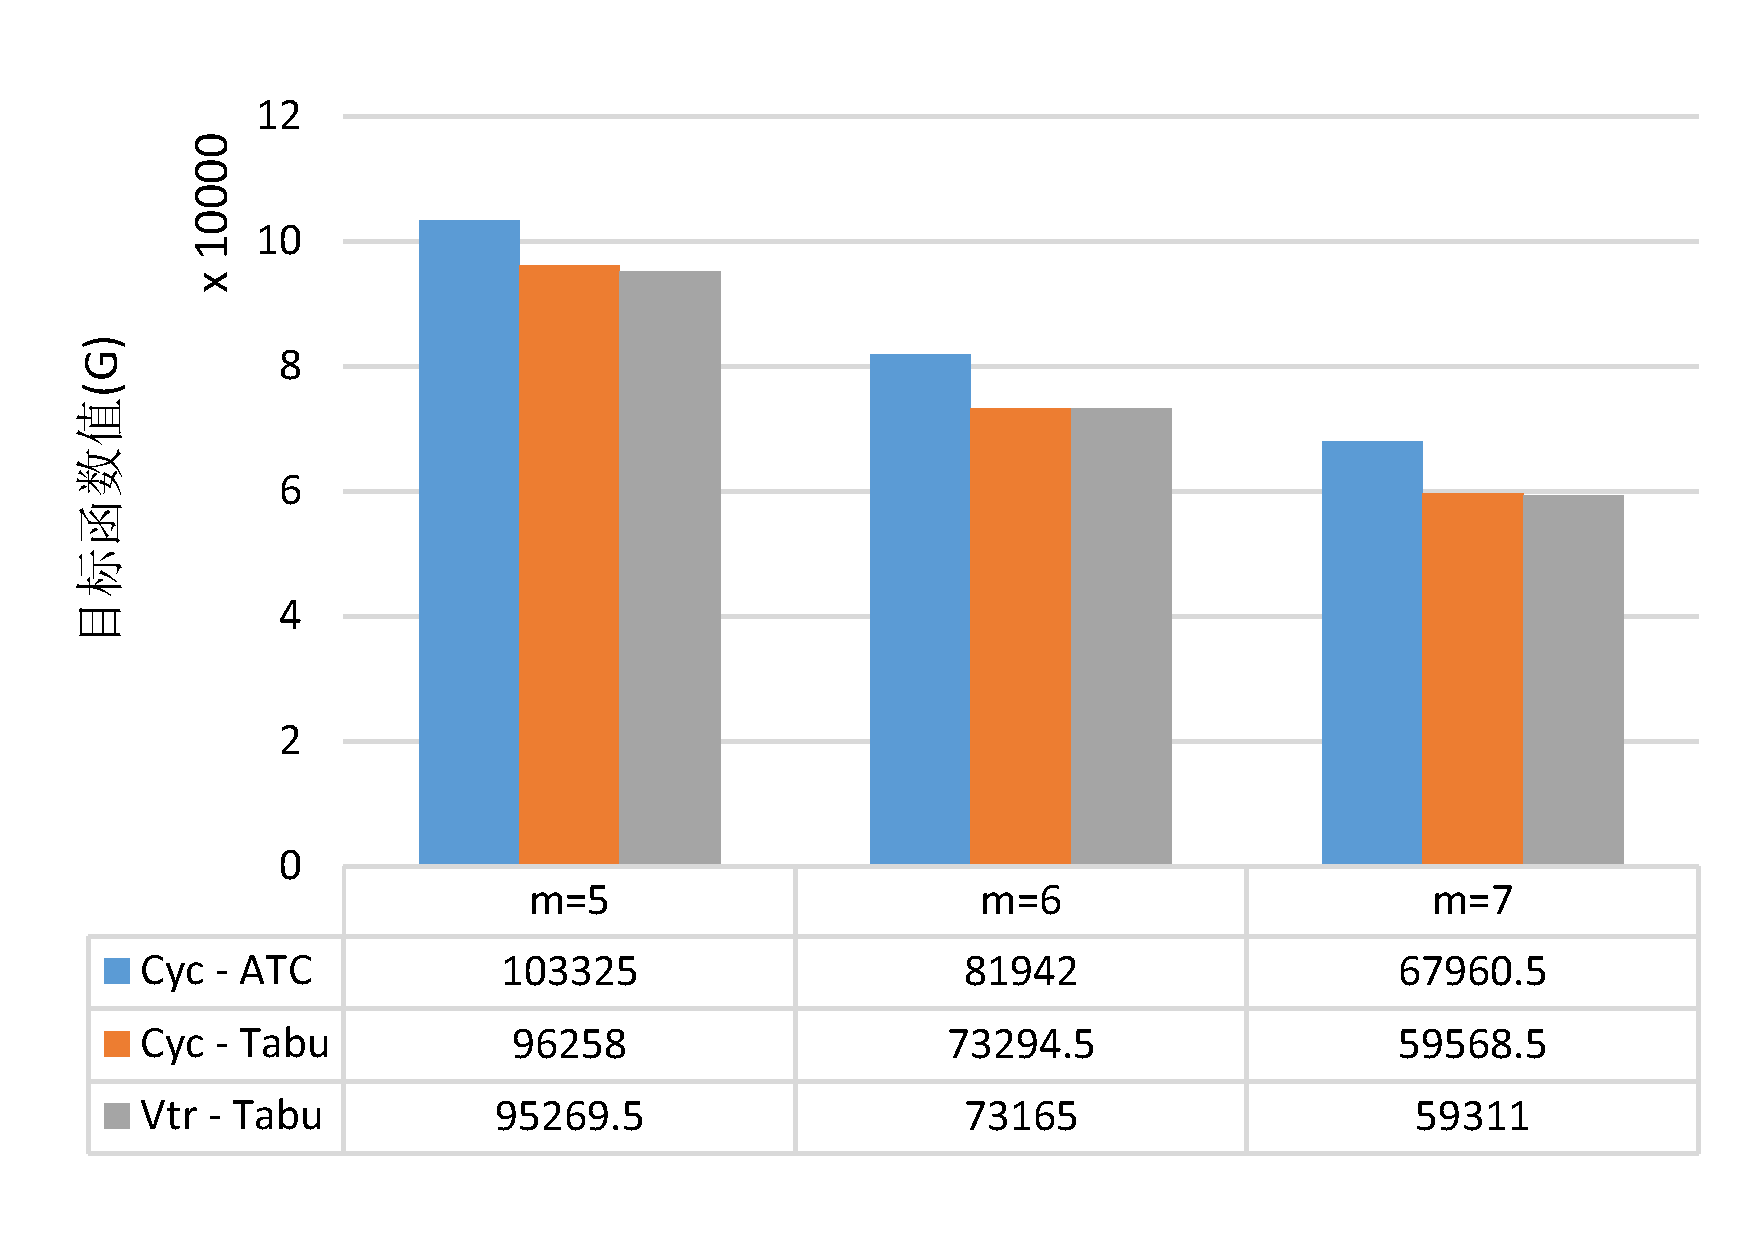
\includegraphics[height = 6cm, angle = -90]{basic_05_100}}
\subfloat[$n = 150$]{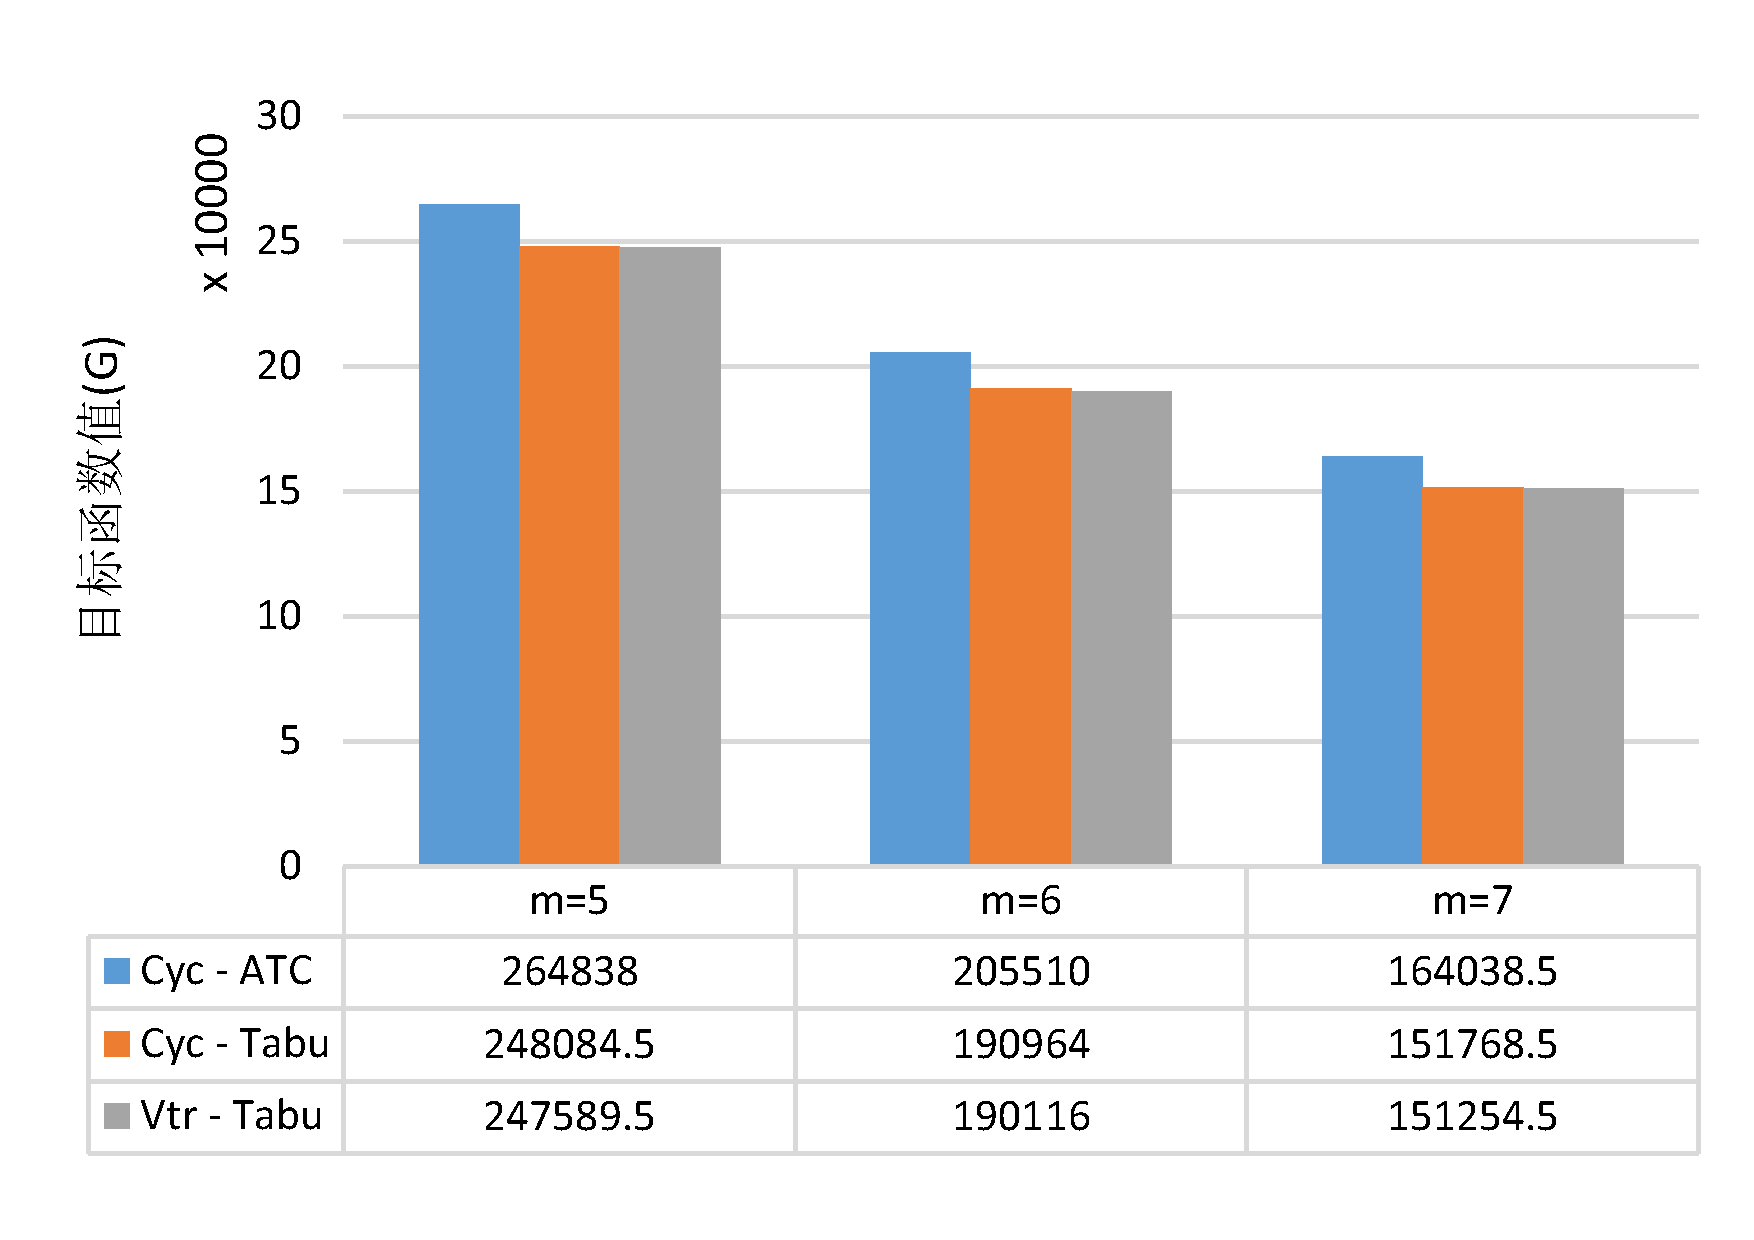
\includegraphics[height = 6cm, angle = -90]{basic_05_150}}
\subfloat[$n = 200$]{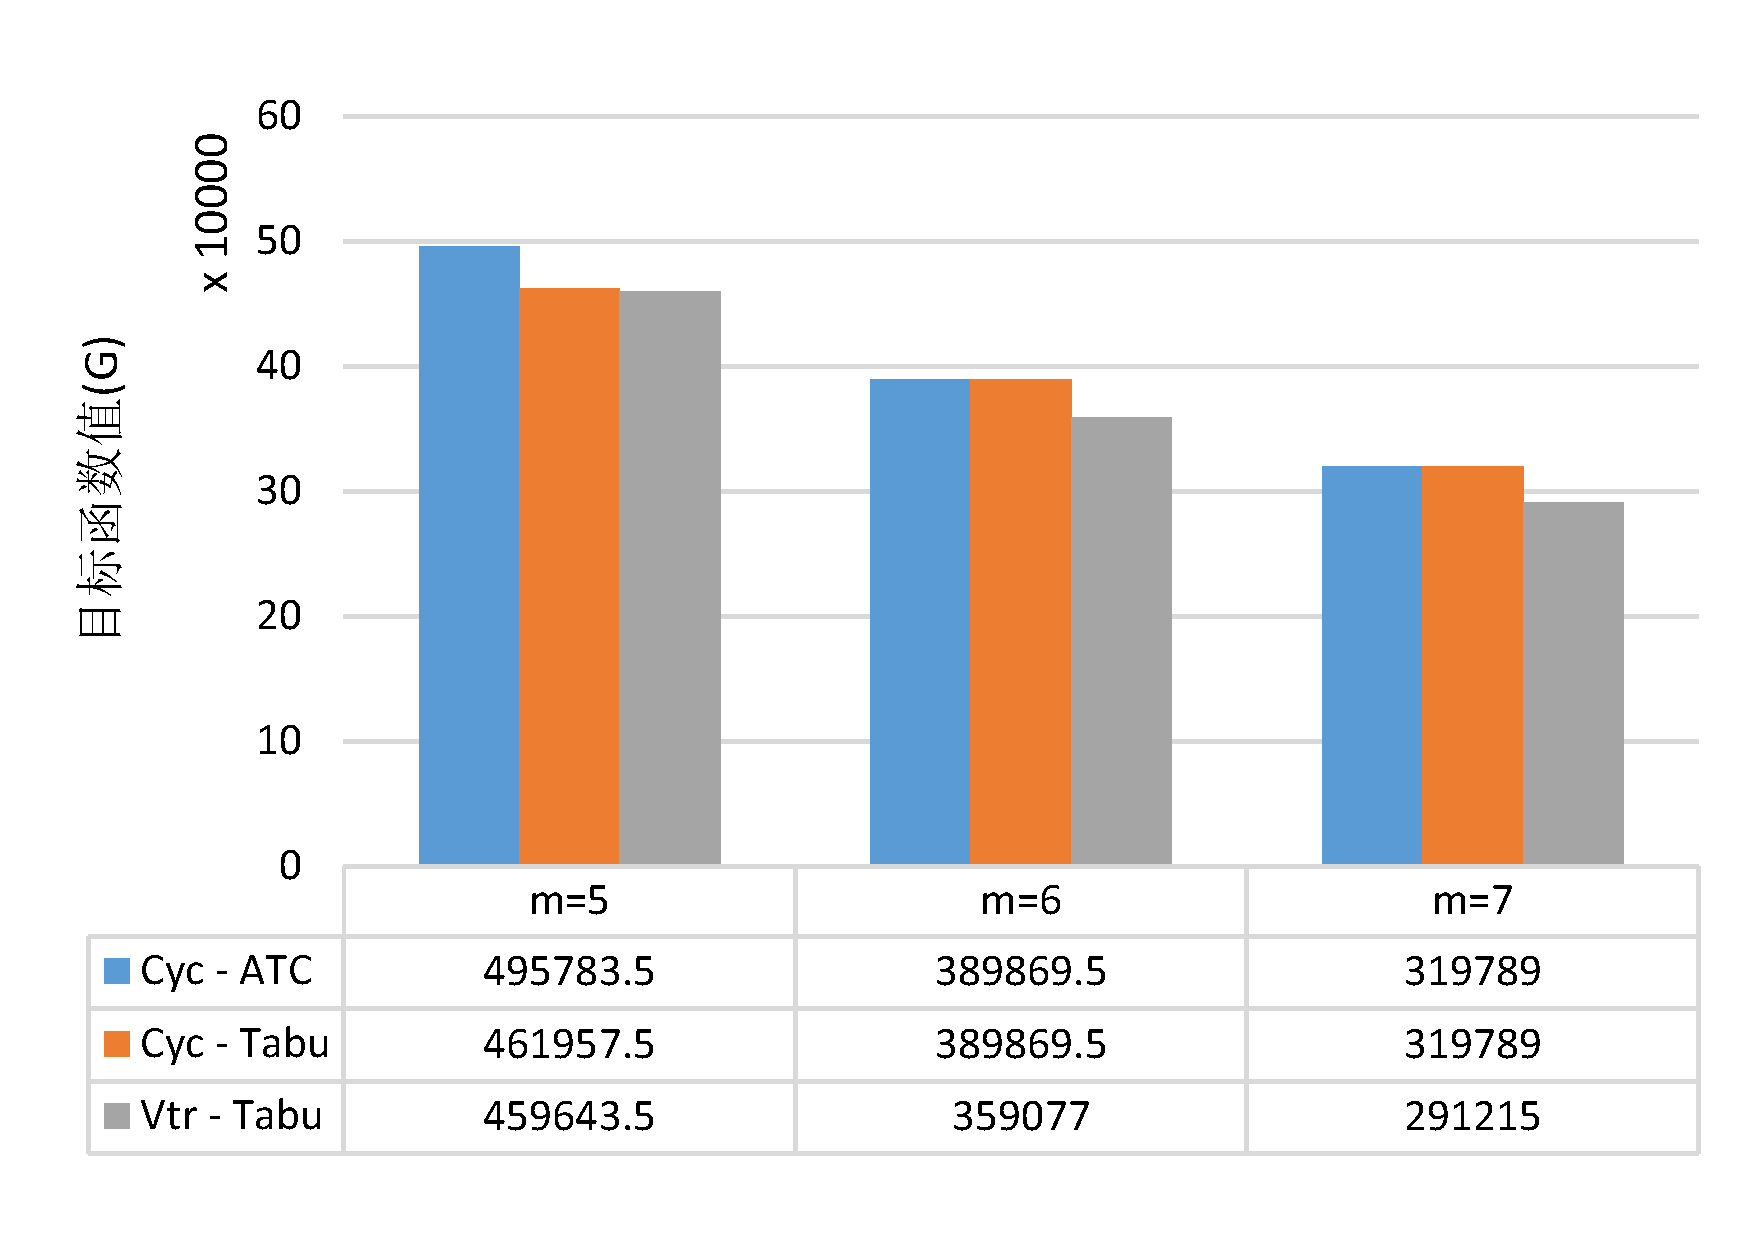
\includegraphics[height = 6cm, angle = -90]{basic_05_200}}
\subfloat[$n = 300$]{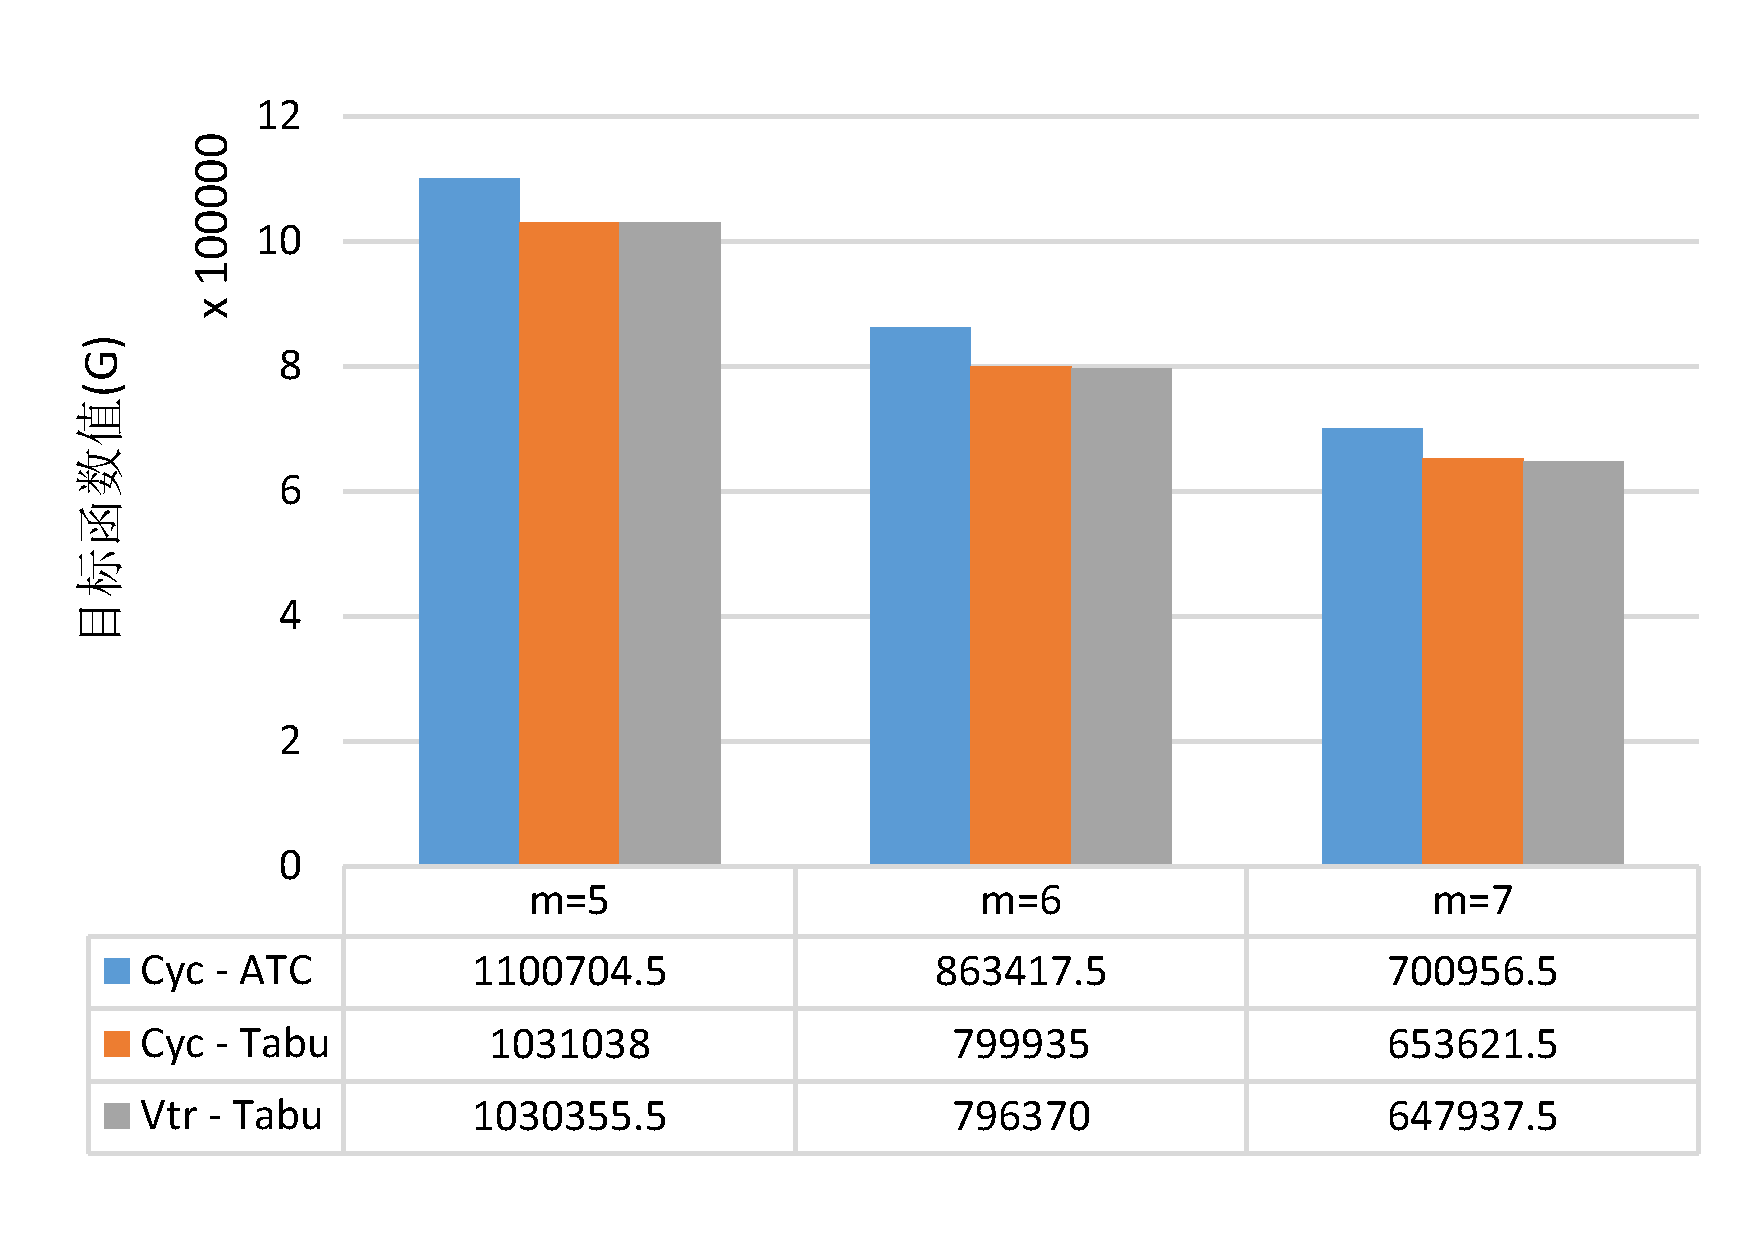
\includegraphics[height = 6cm, angle = -90]{basic_05_300}}\\
\subfloat[$n = 500$]{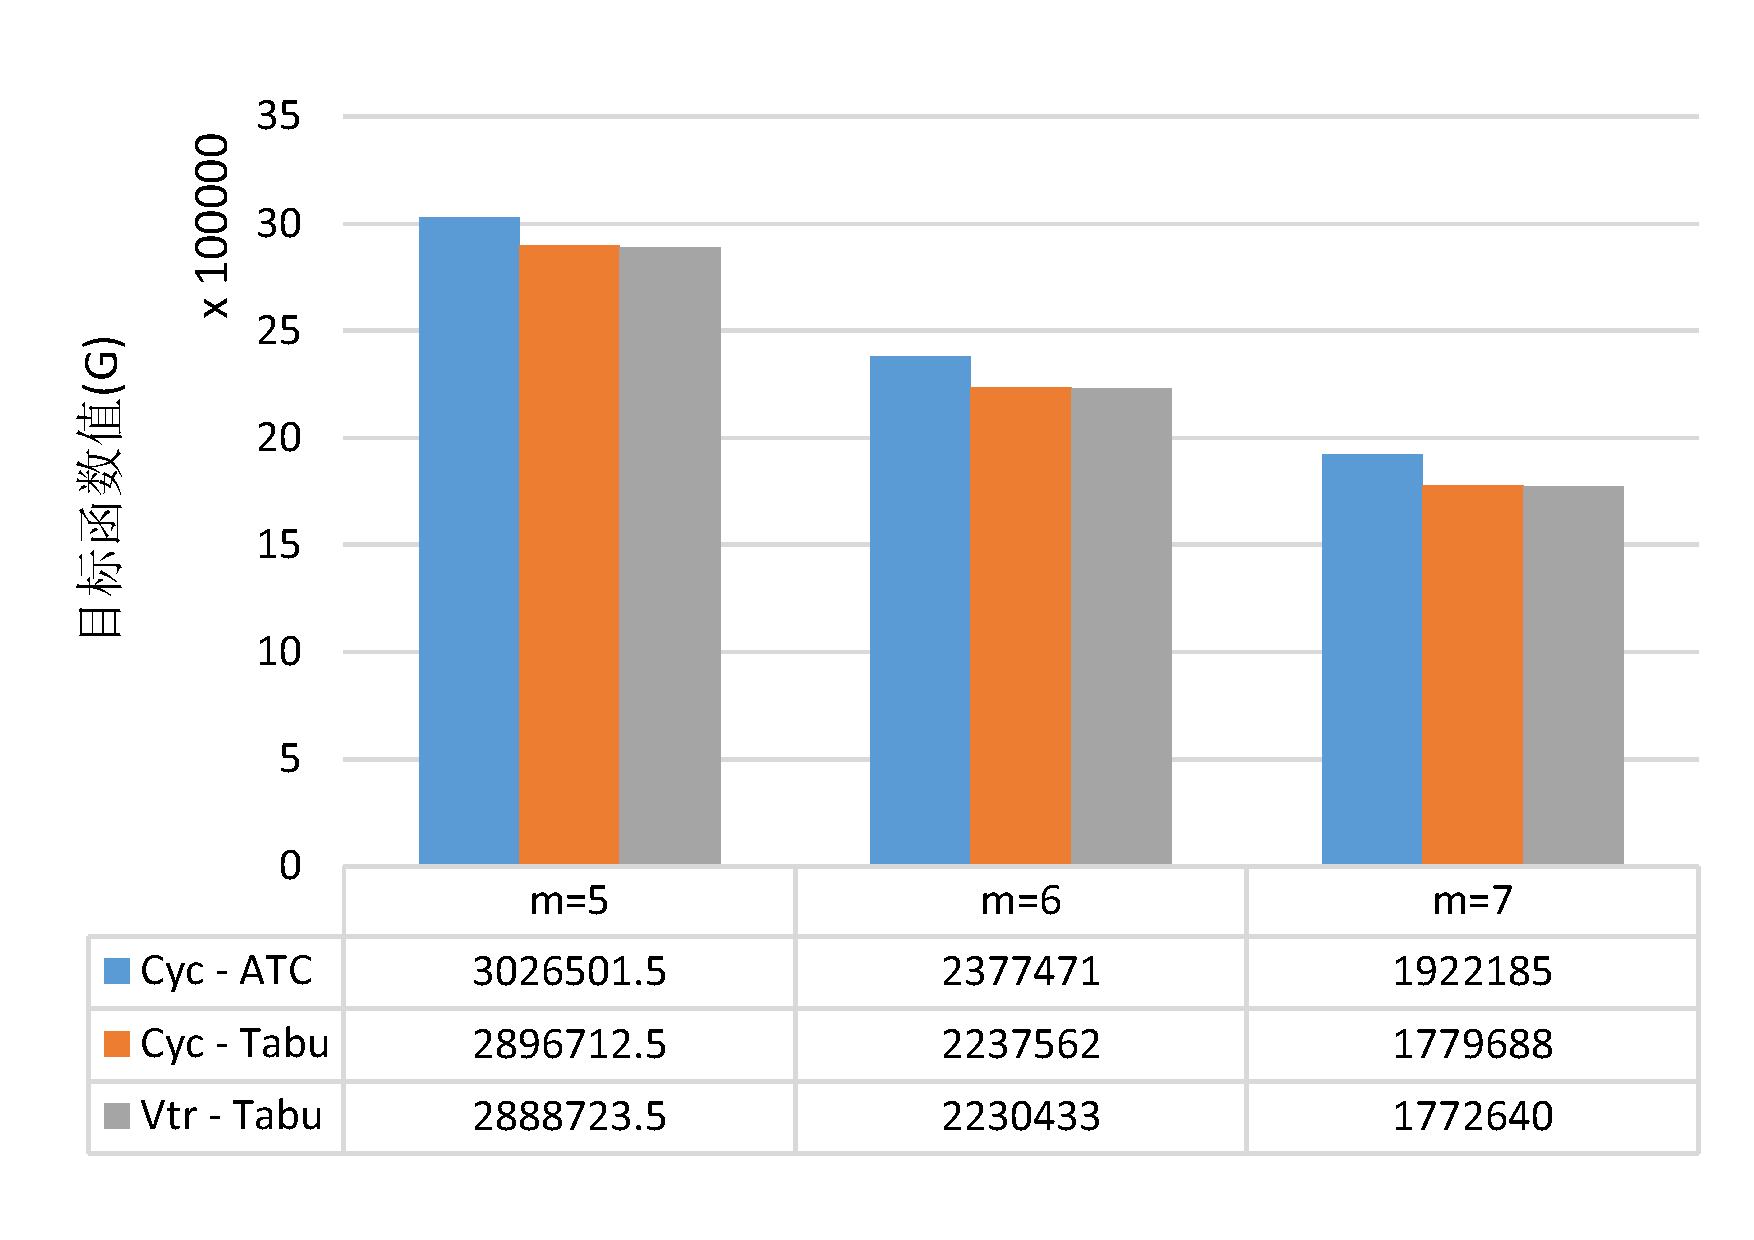
\includegraphics[height = 6cm, angle = -90]{basic_05_500}}
\subfloat[$n = 750$]{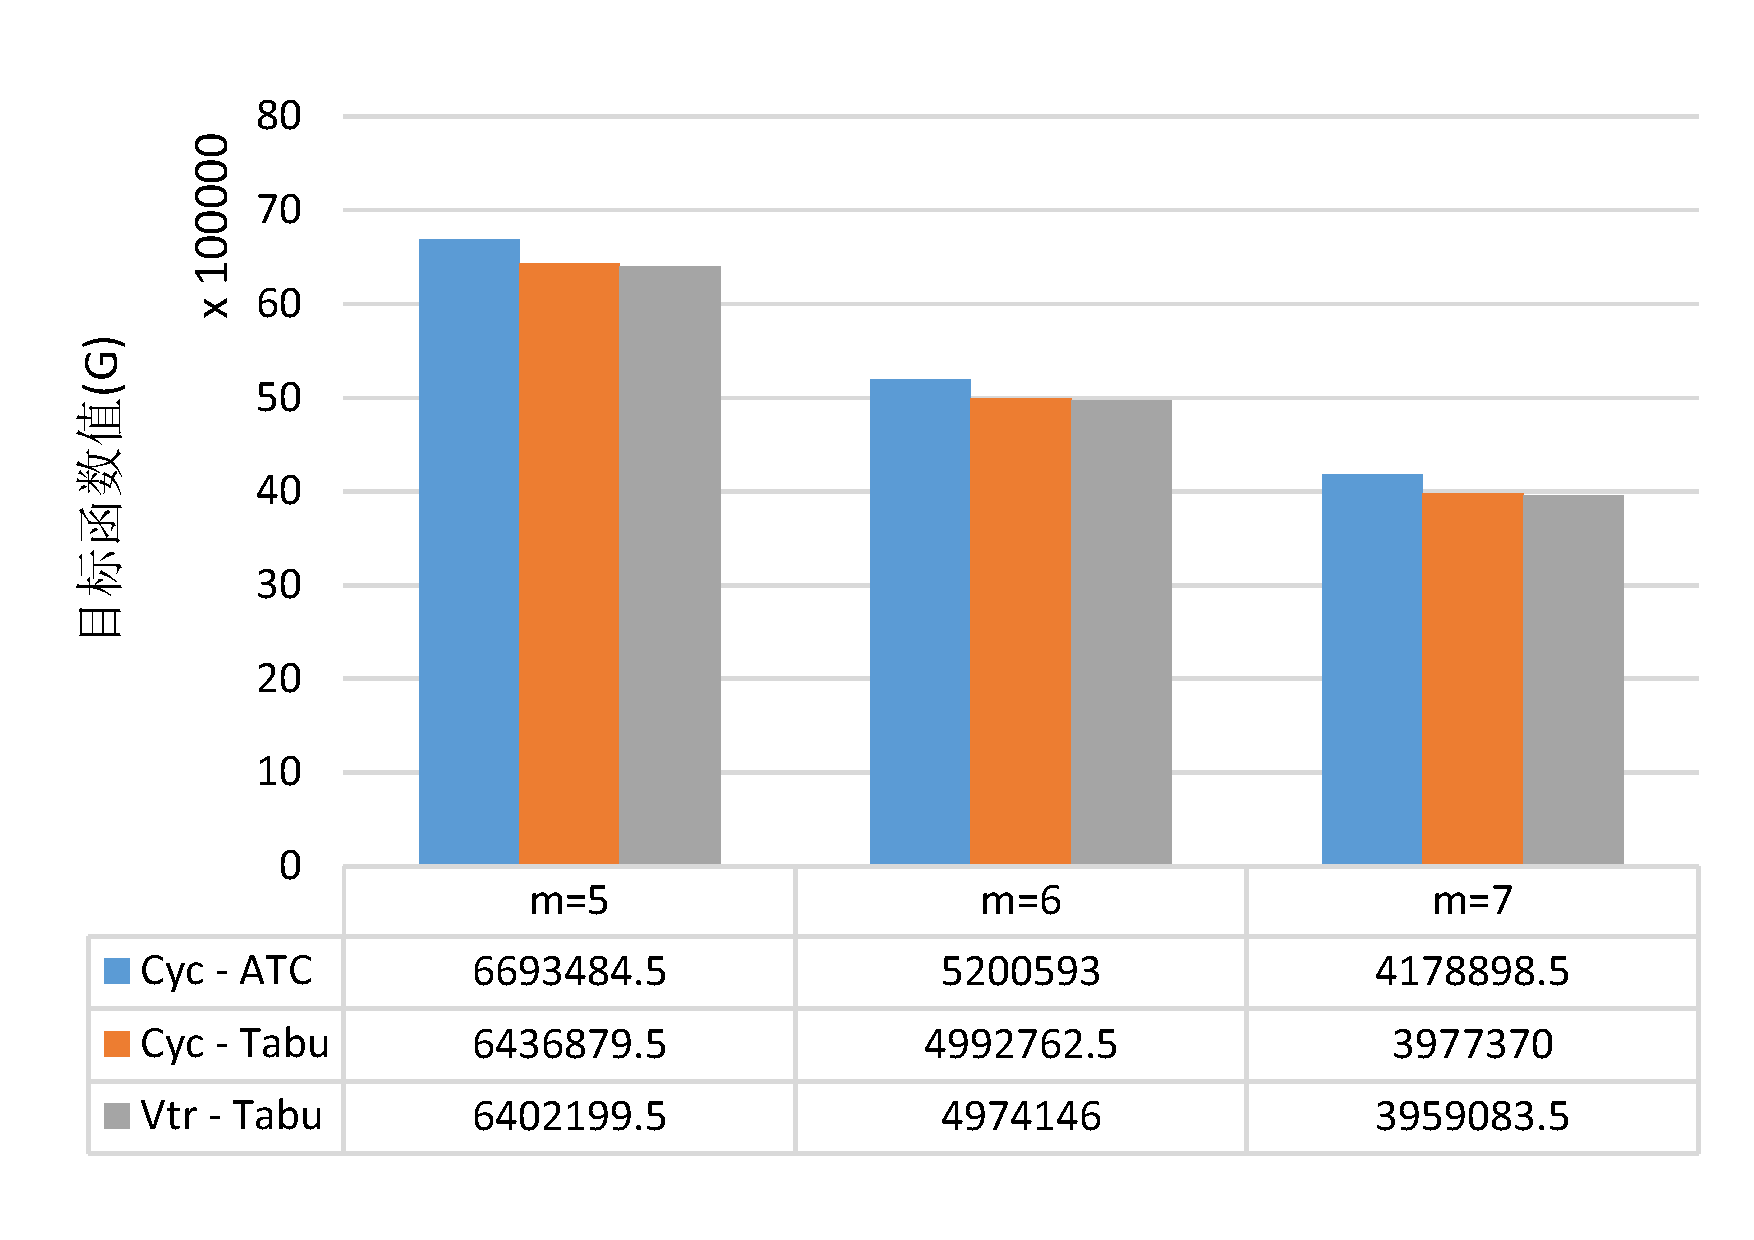
\includegraphics[height = 6cm, angle = -90]{basic_05_750}}
\subfloat[$n = 1000$]{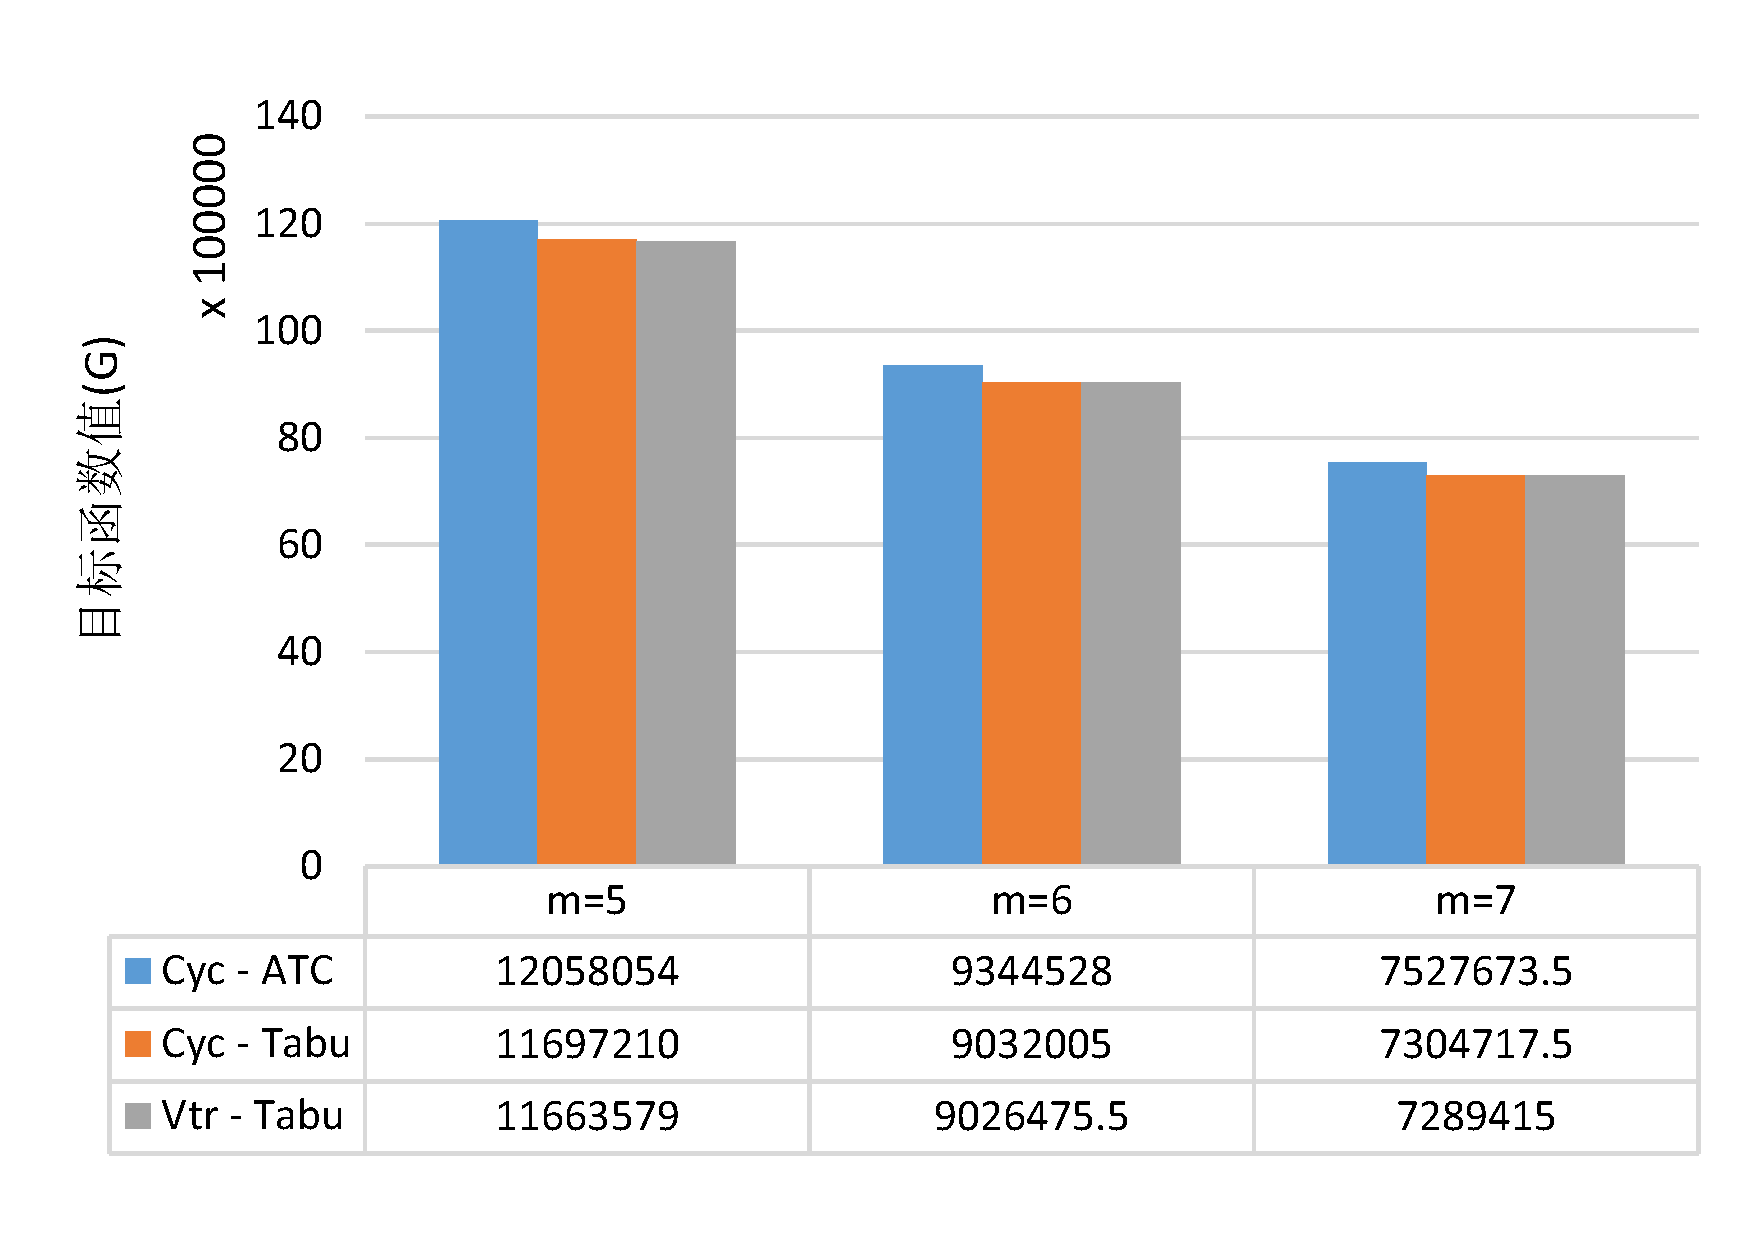
\includegraphics[height = 6cm, angle = -90]{basic_05_1000}}
\caption{\label{fig:result2}模型$1$的Cyc -- ATC、Cyc -- Tabu、Vtr -- Tabu 算法求解目标函数值比较$(\lambda_1 = 0.5)$}
\end{sidewaysfigure}

\begin{sidewaysfigure}
\centering
\subfloat[$n = 20$]{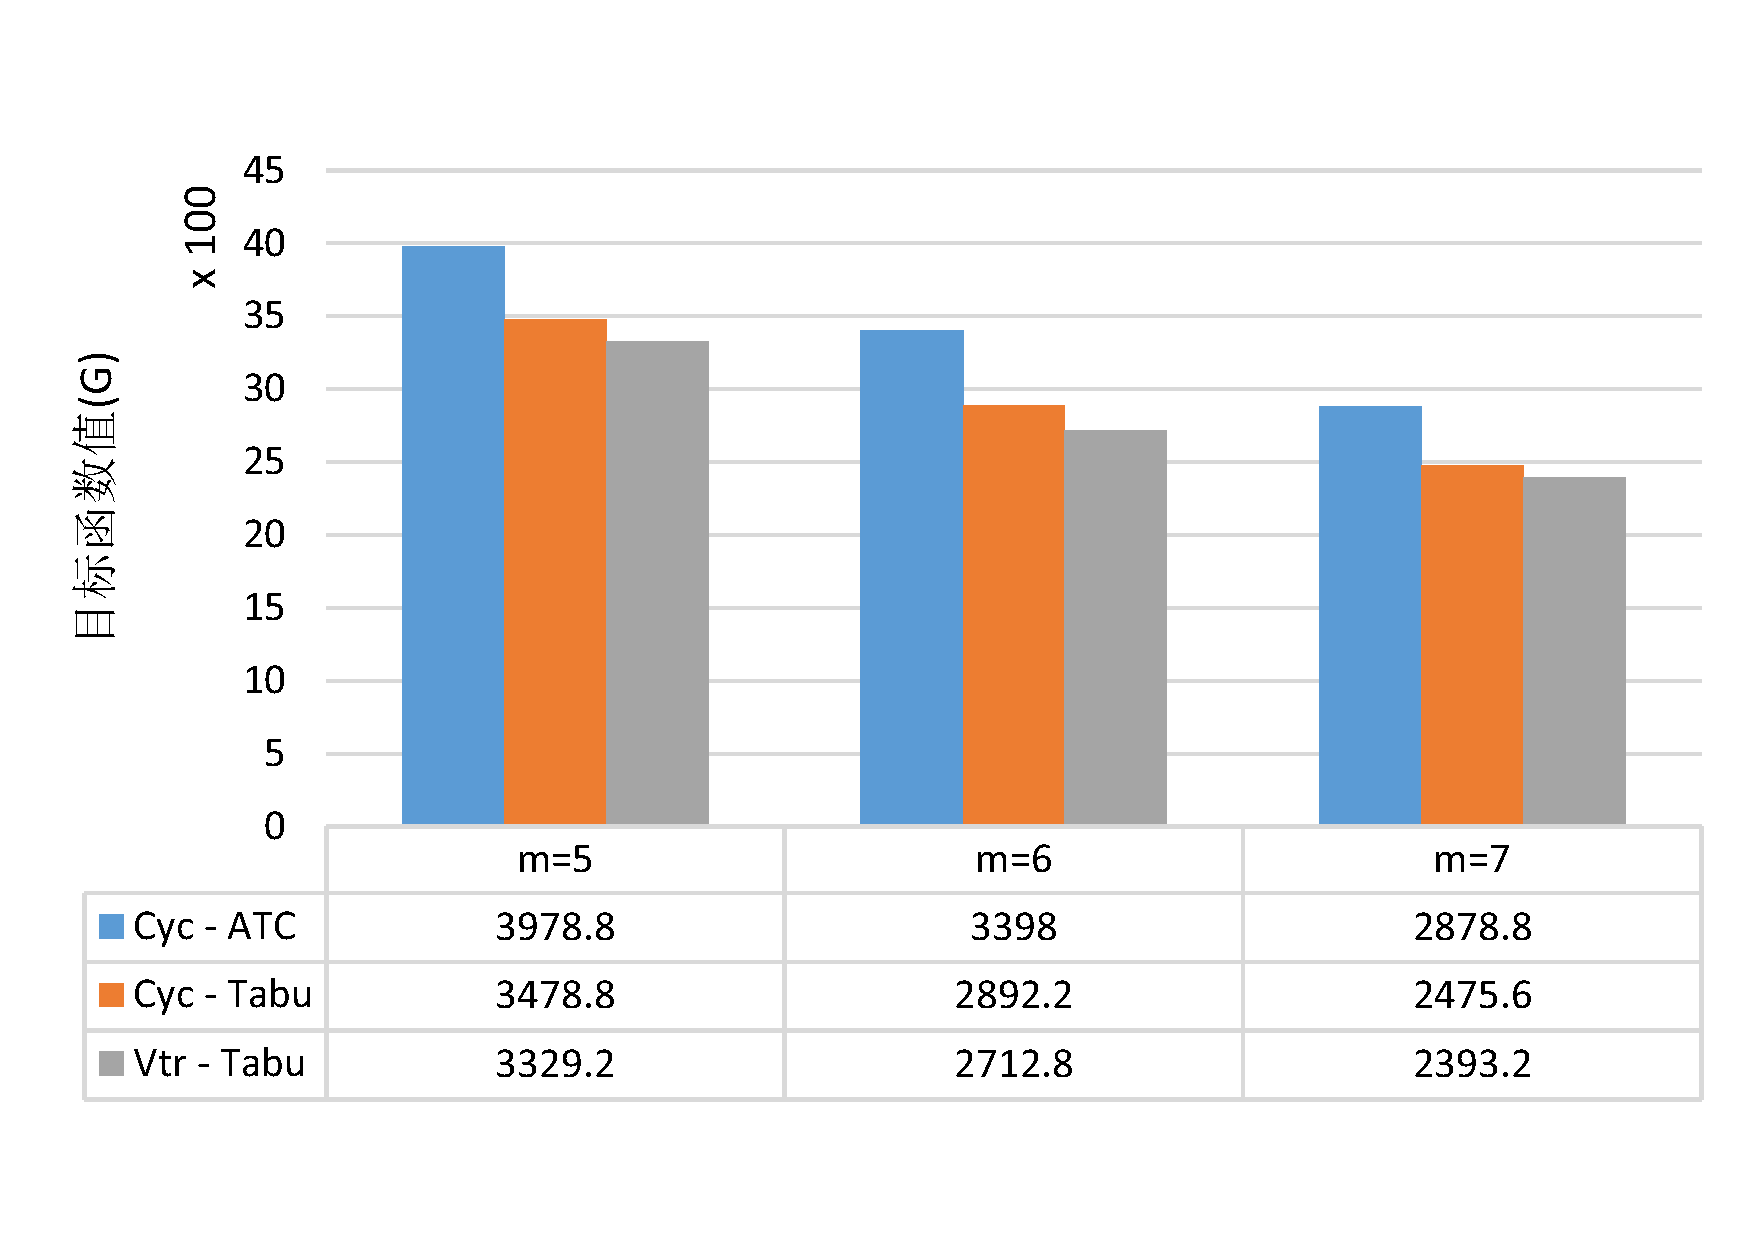
\includegraphics[height = 6cm, angle = -90]{basic_06_20}}
\subfloat[$n = 30$]{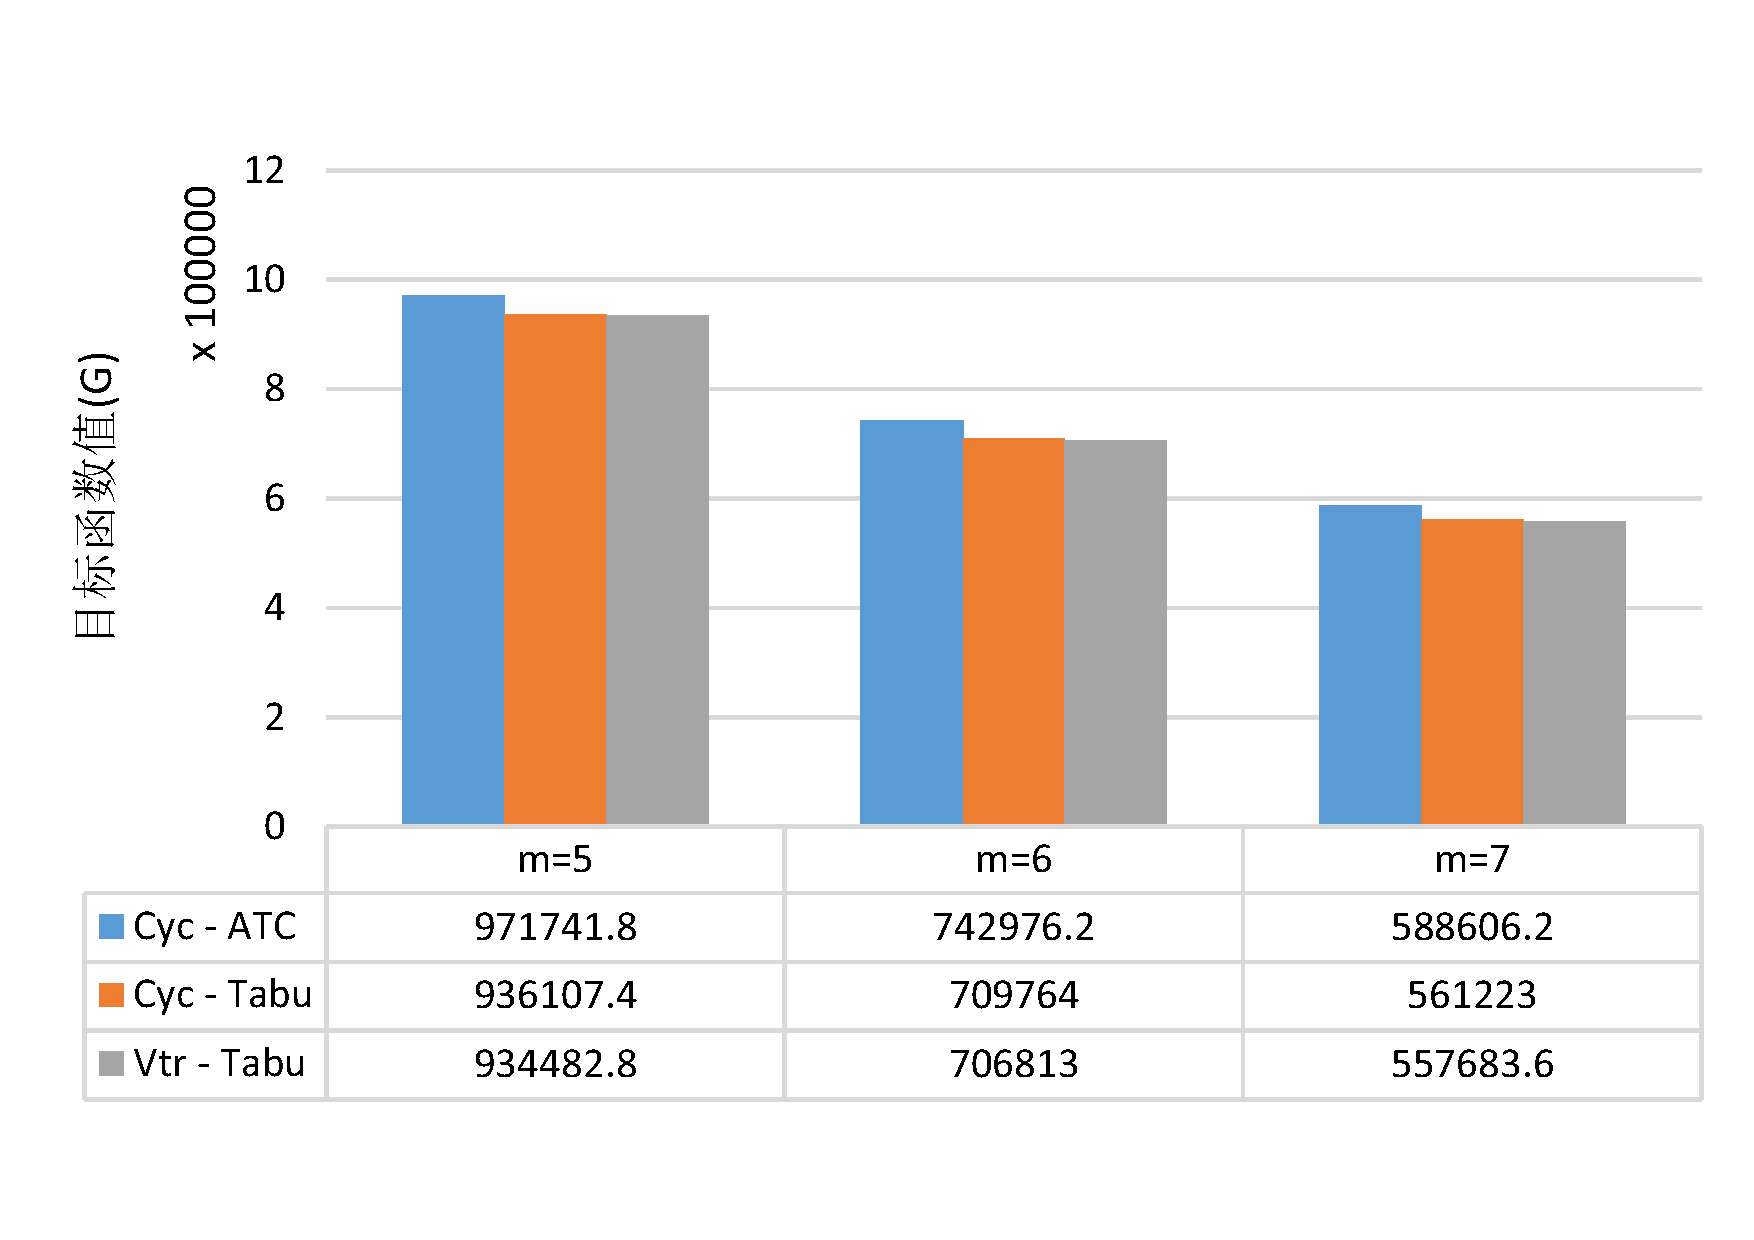
\includegraphics[height = 6cm, angle = -90]{basic_06_300}}
\subfloat[$n = 50$]{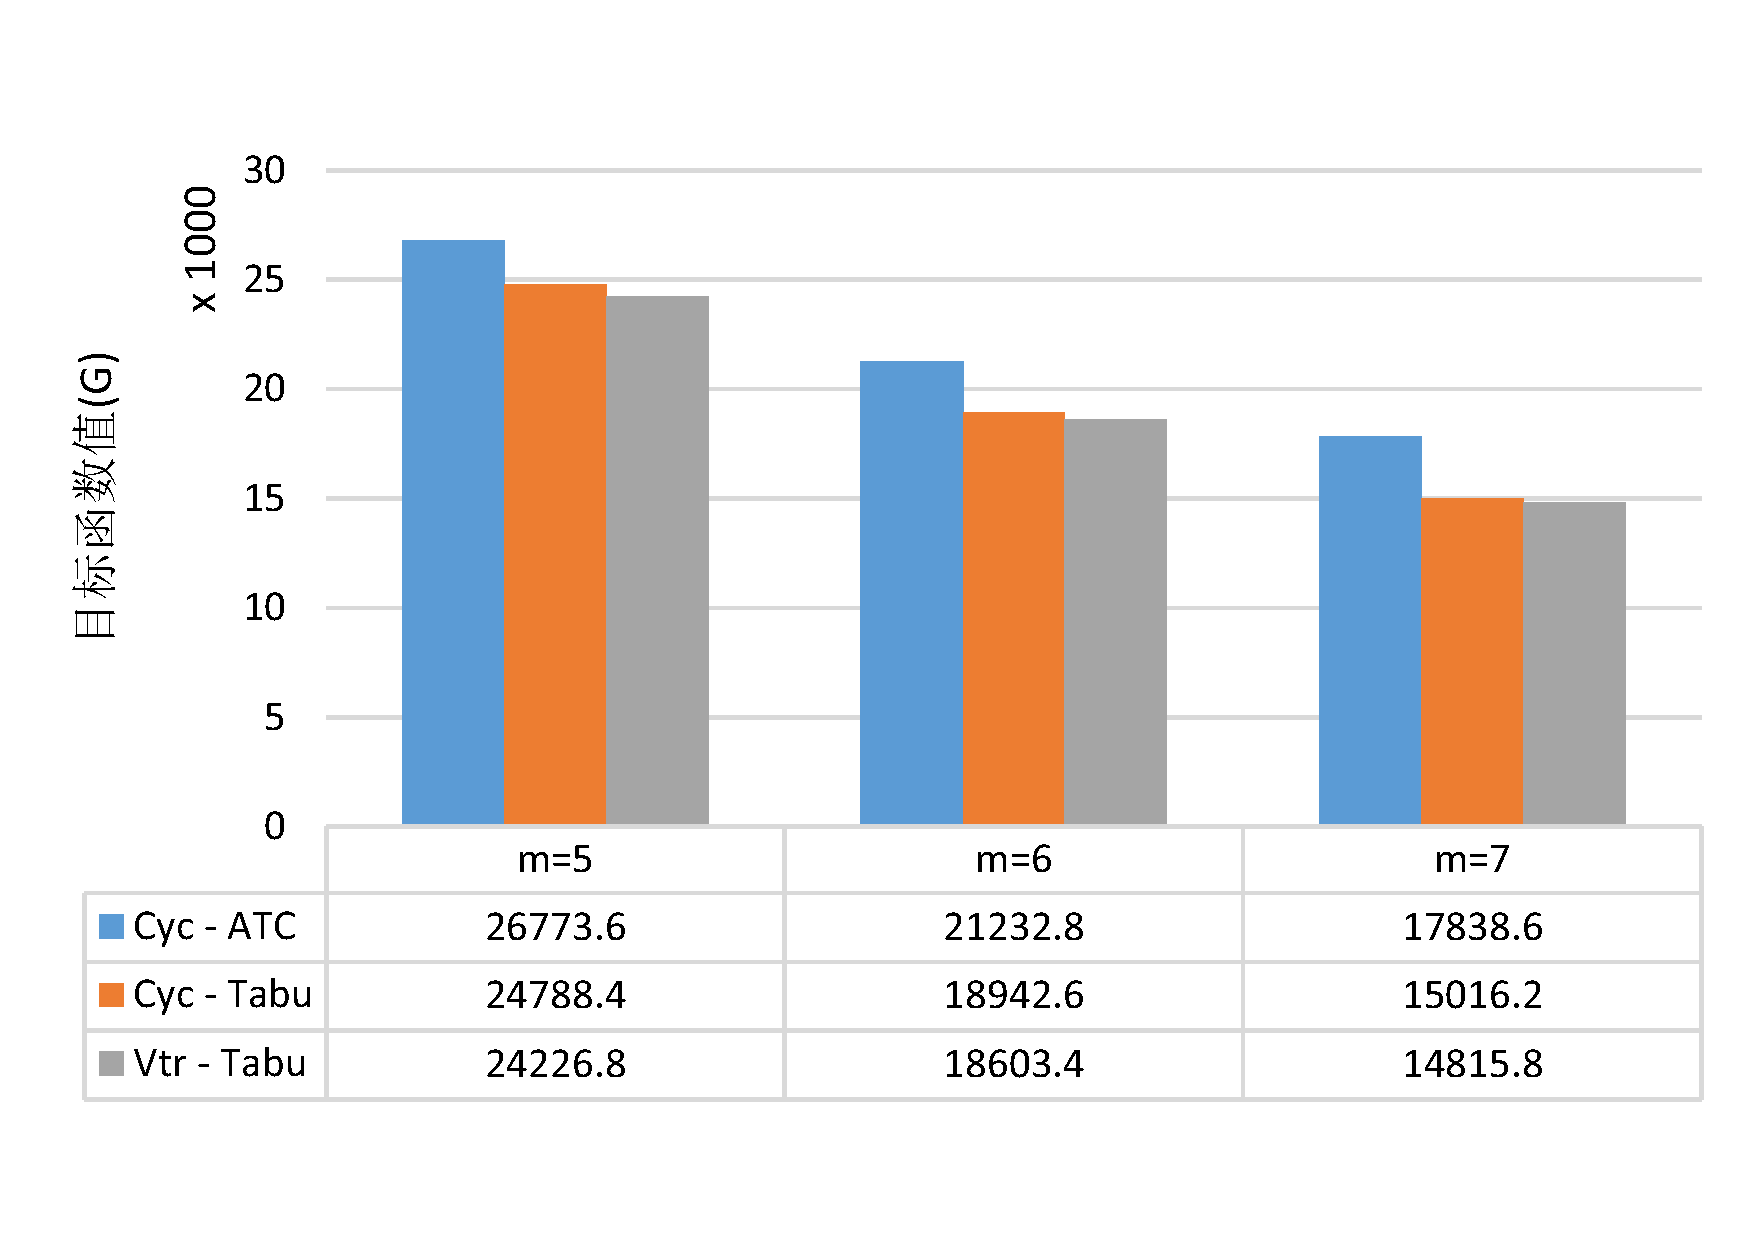
\includegraphics[height = 6cm, angle = -90]{basic_06_50}}
\subfloat[$n = 70$]{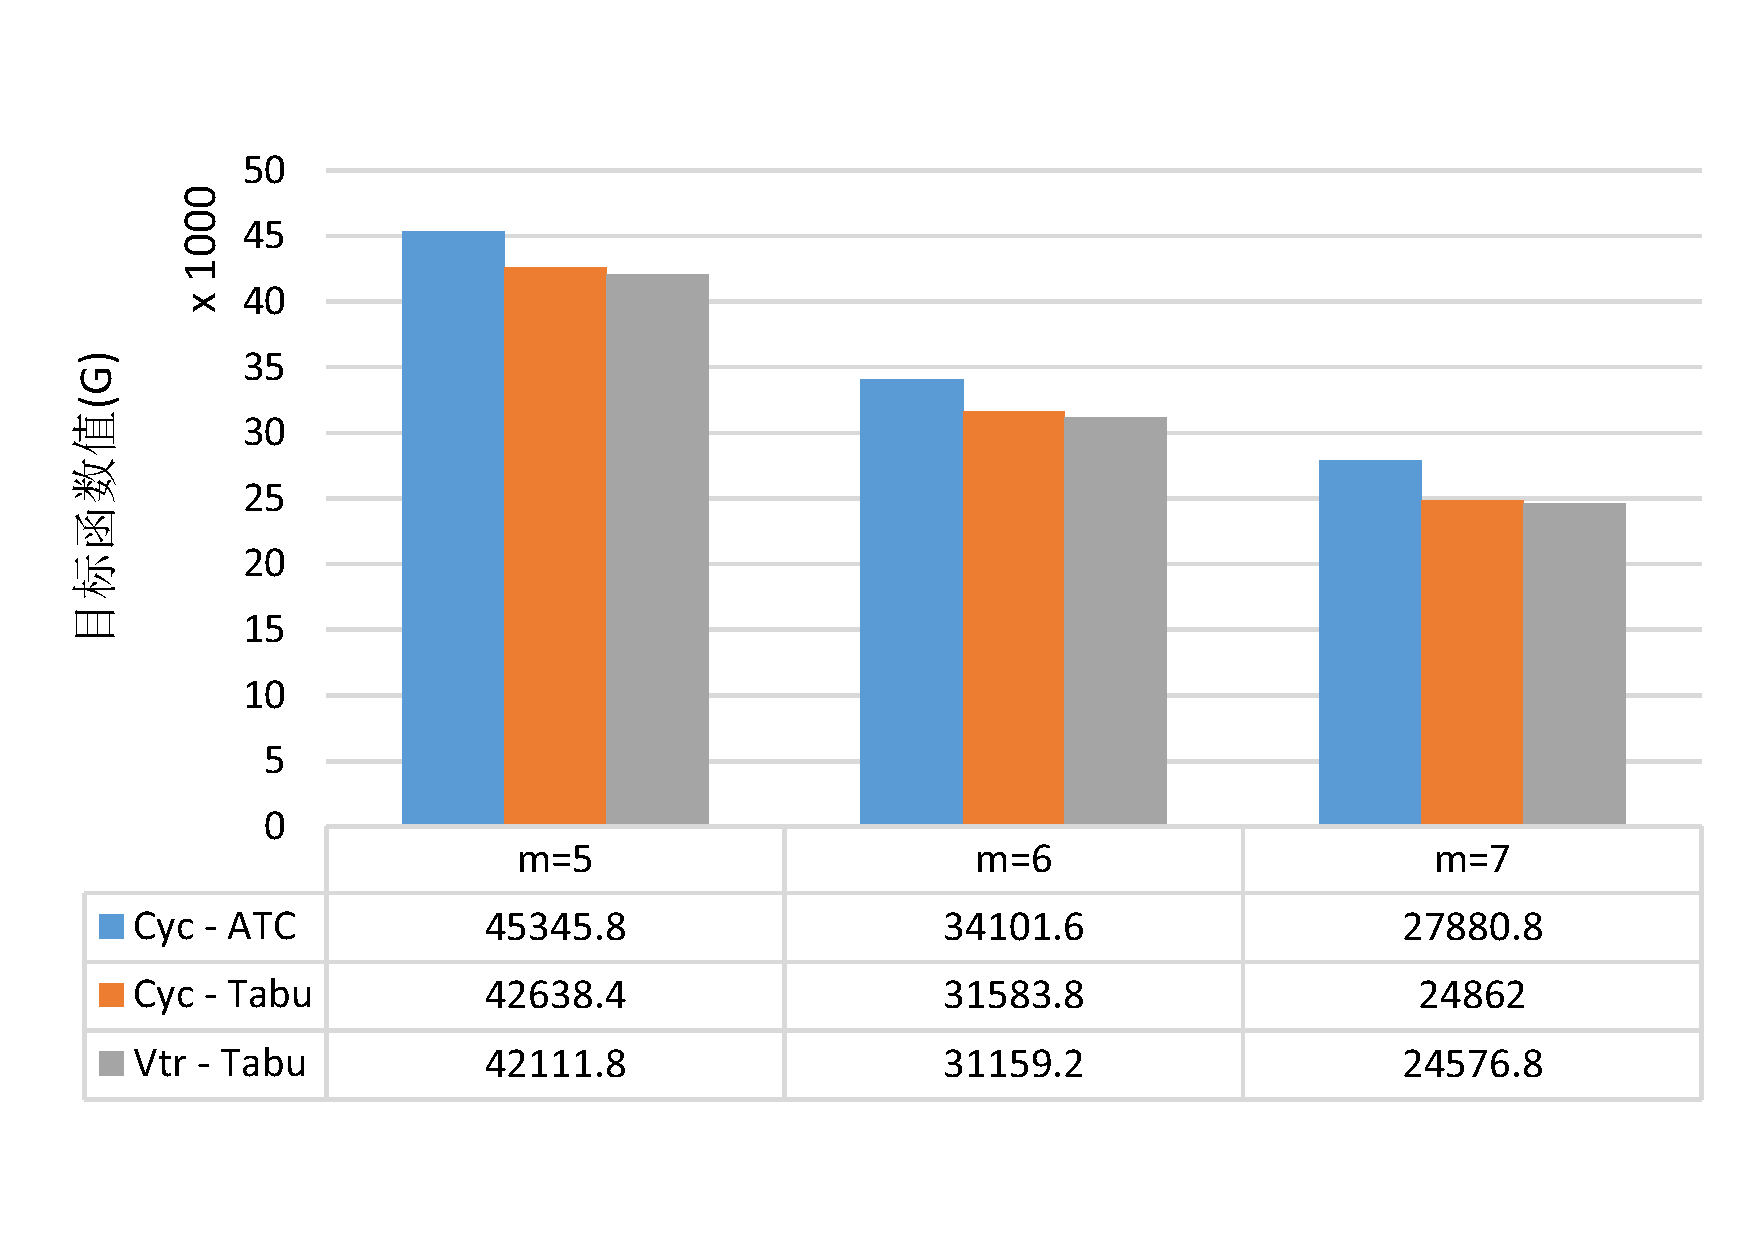
\includegraphics[height = 6cm, angle = -90]{basic_06_70}}\\
\subfloat[$n = 100$]{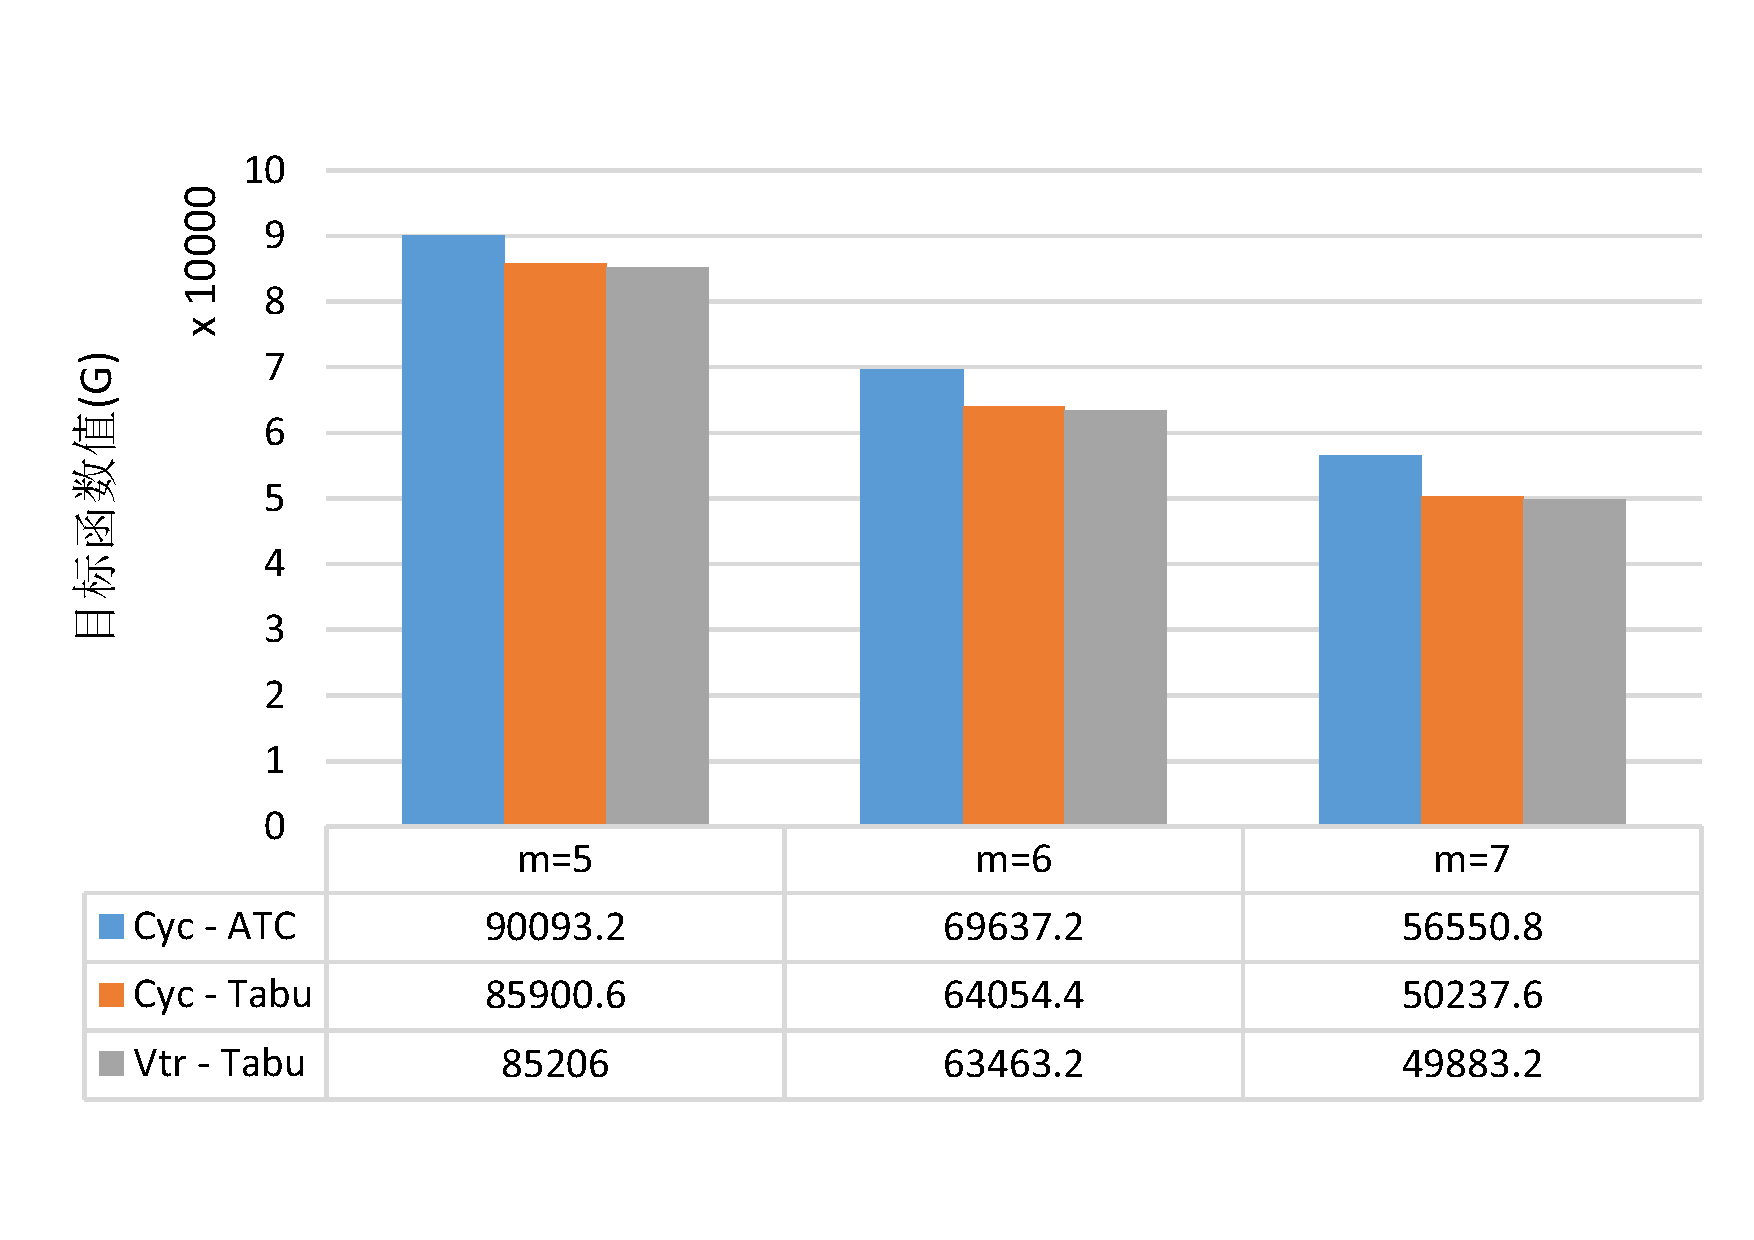
\includegraphics[height = 6cm, angle = -90]{basic_06_100}}
\subfloat[$n = 150$]{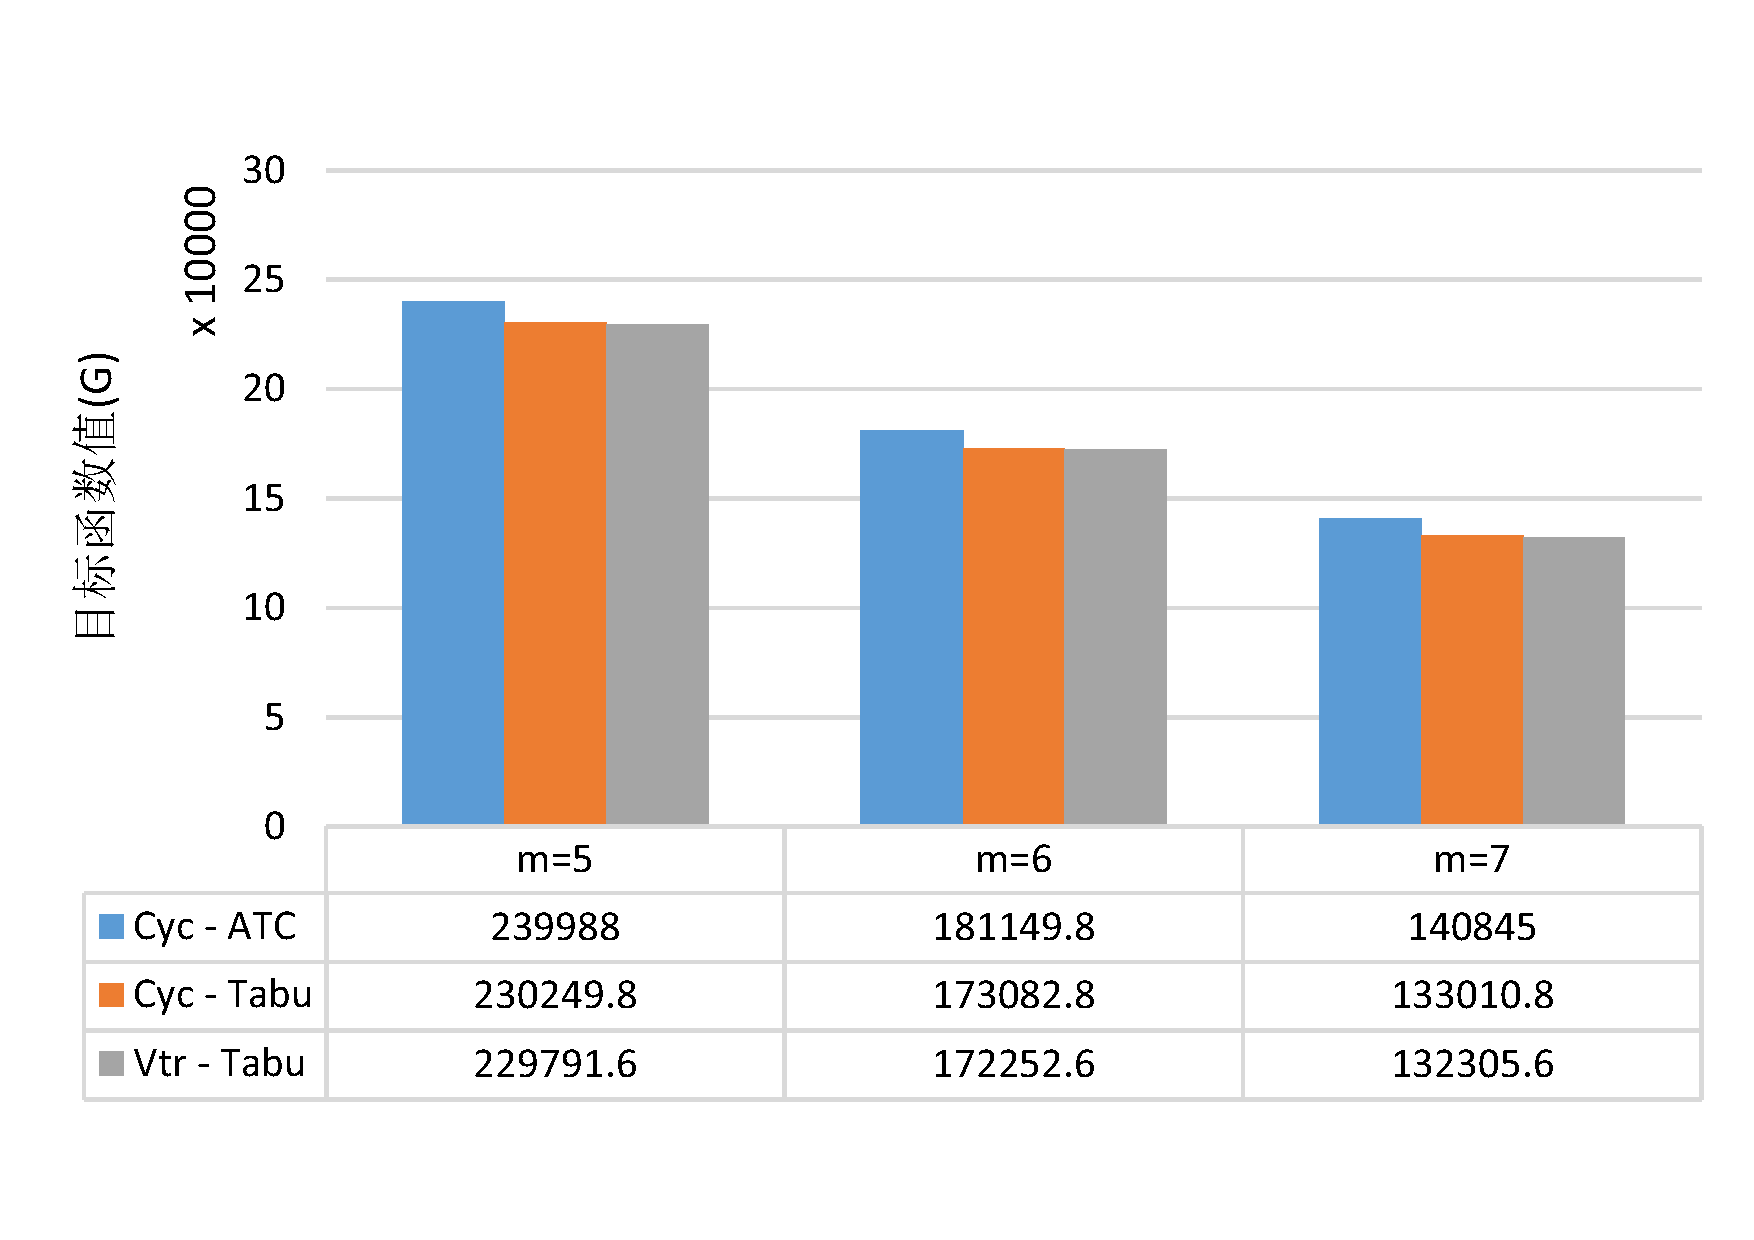
\includegraphics[height = 6cm, angle = -90]{basic_06_150}}
\subfloat[$n = 200$]{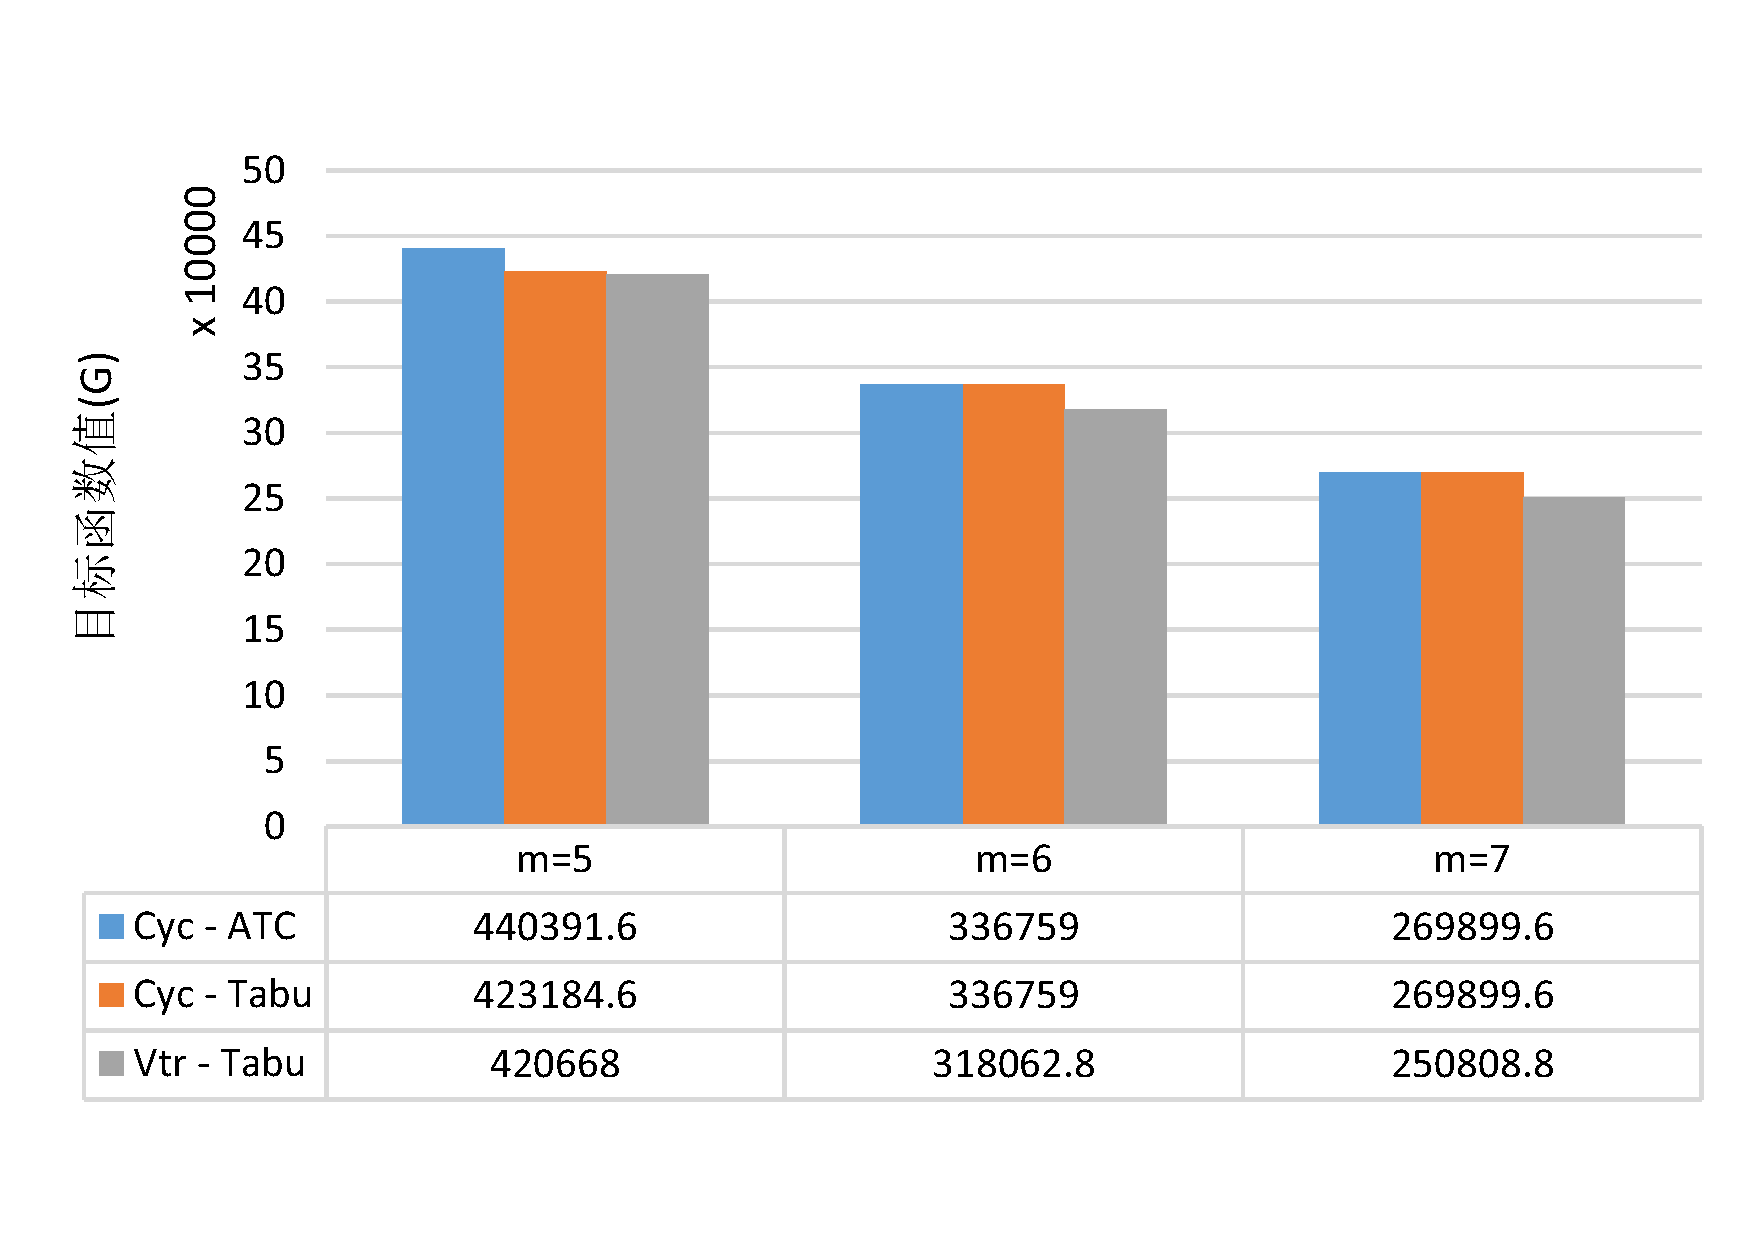
\includegraphics[height = 6cm, angle = -90]{basic_06_200}}
\subfloat[$n = 300$]{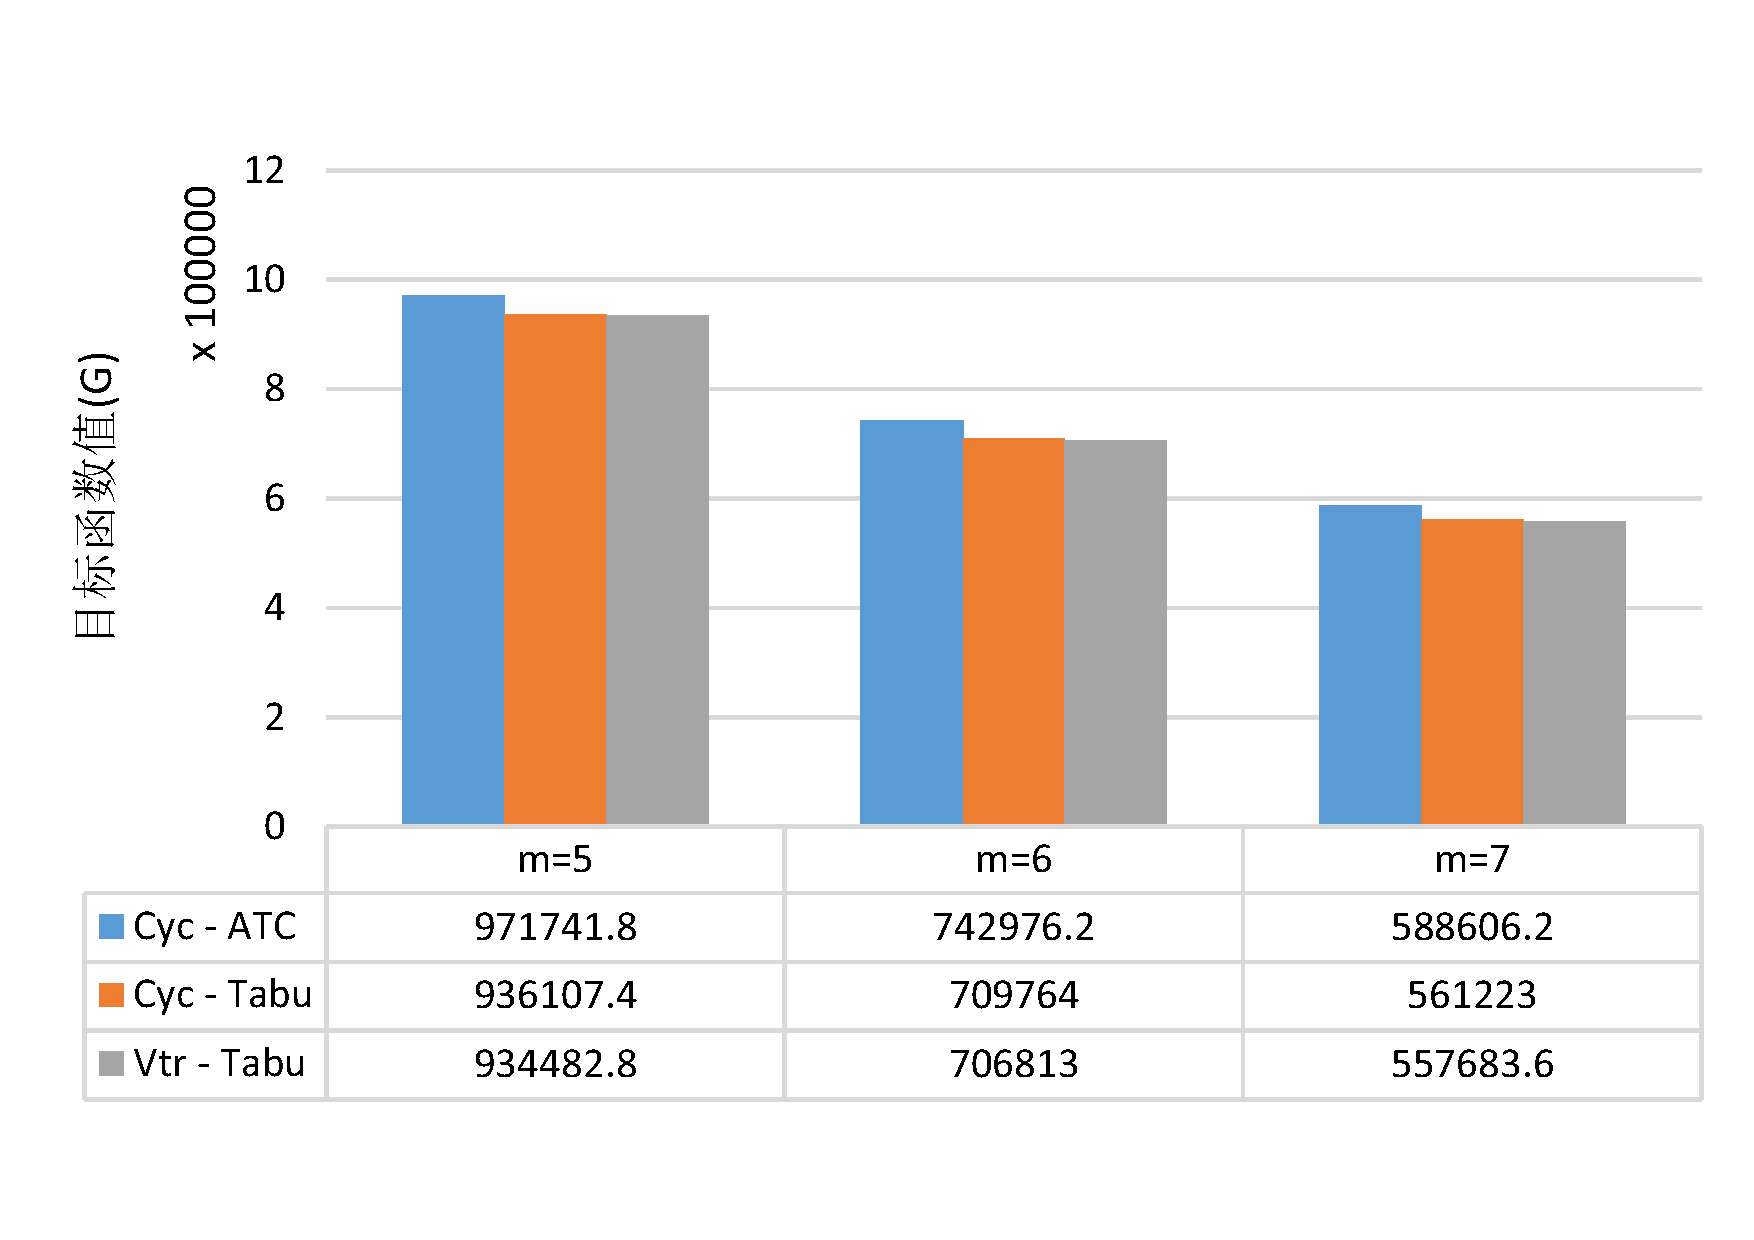
\includegraphics[height = 6cm, angle = -90]{basic_06_300}}\\
\subfloat[$n = 500$]{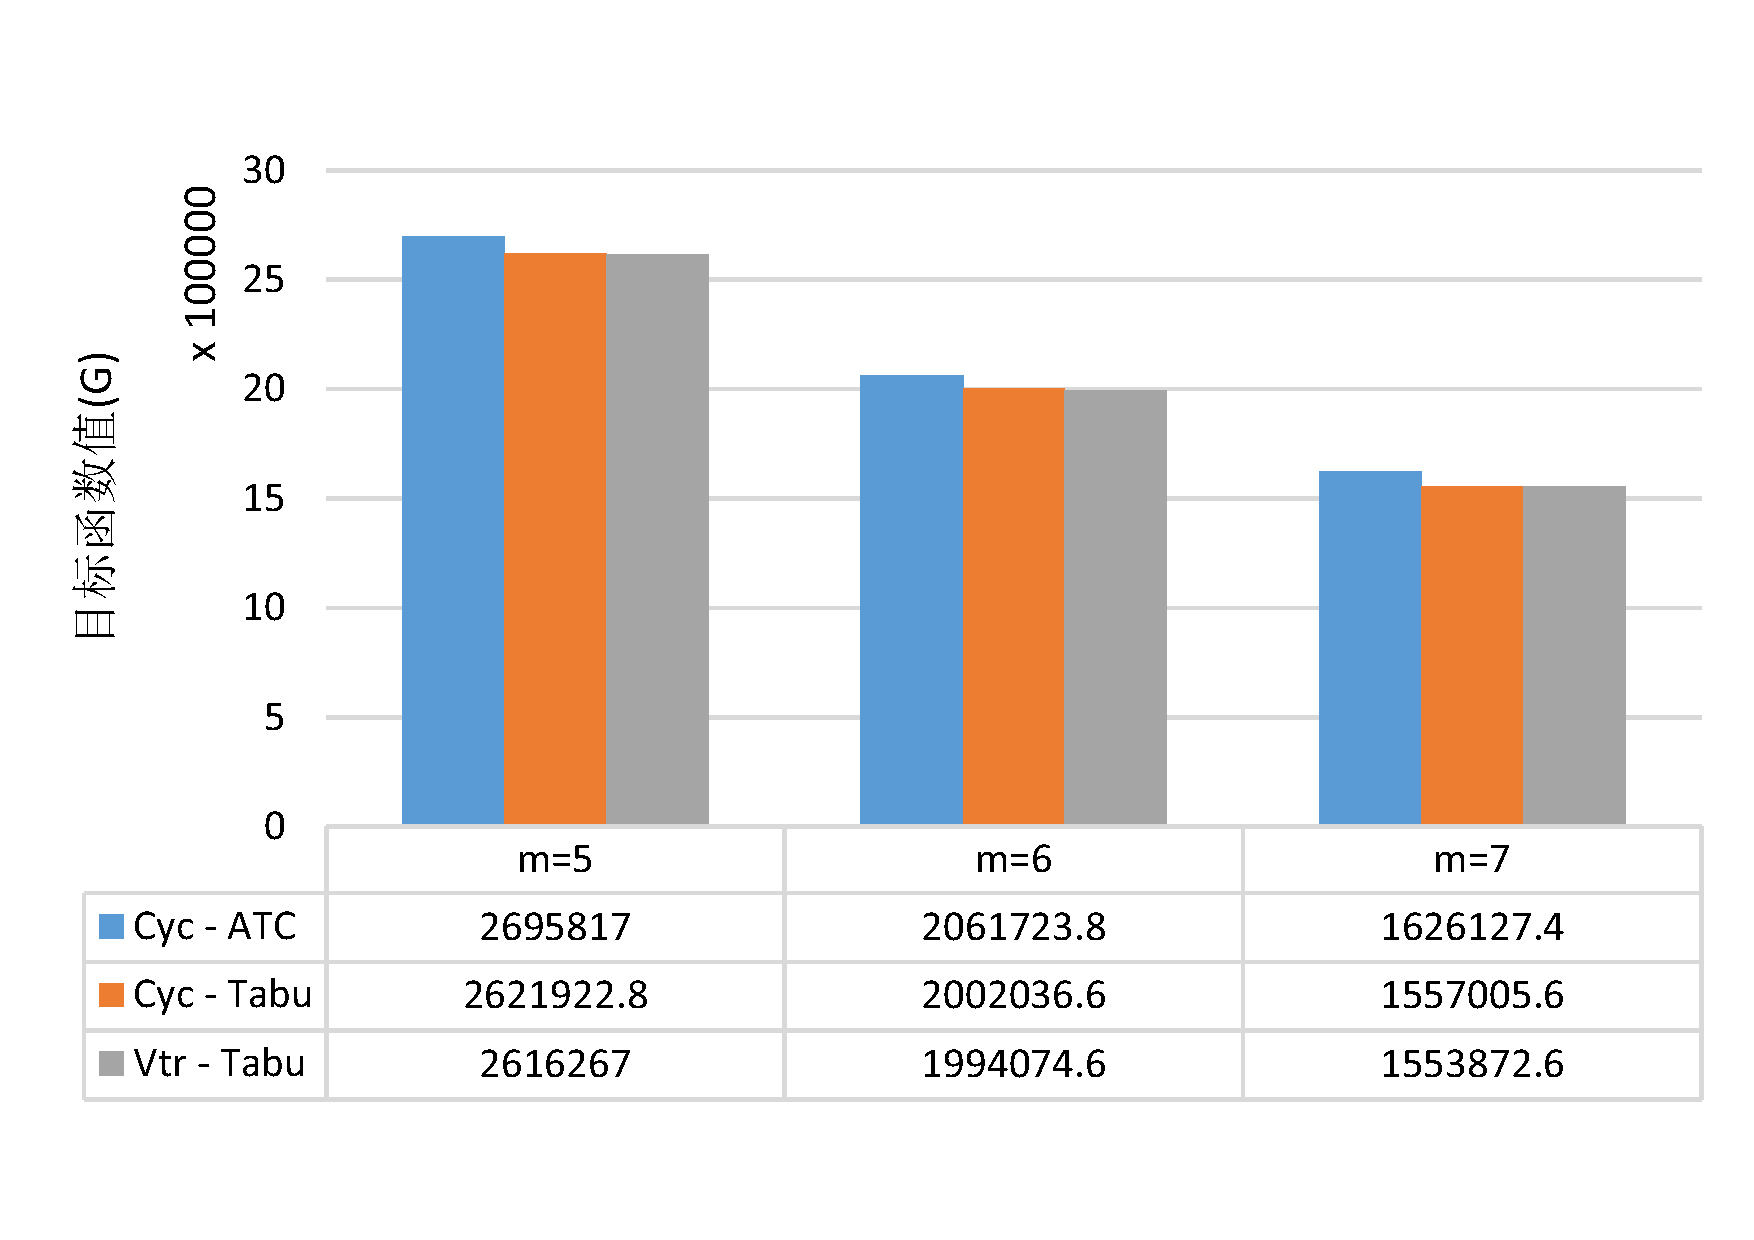
\includegraphics[height = 6cm, angle = -90]{basic_06_500}}
\subfloat[$n = 750$]{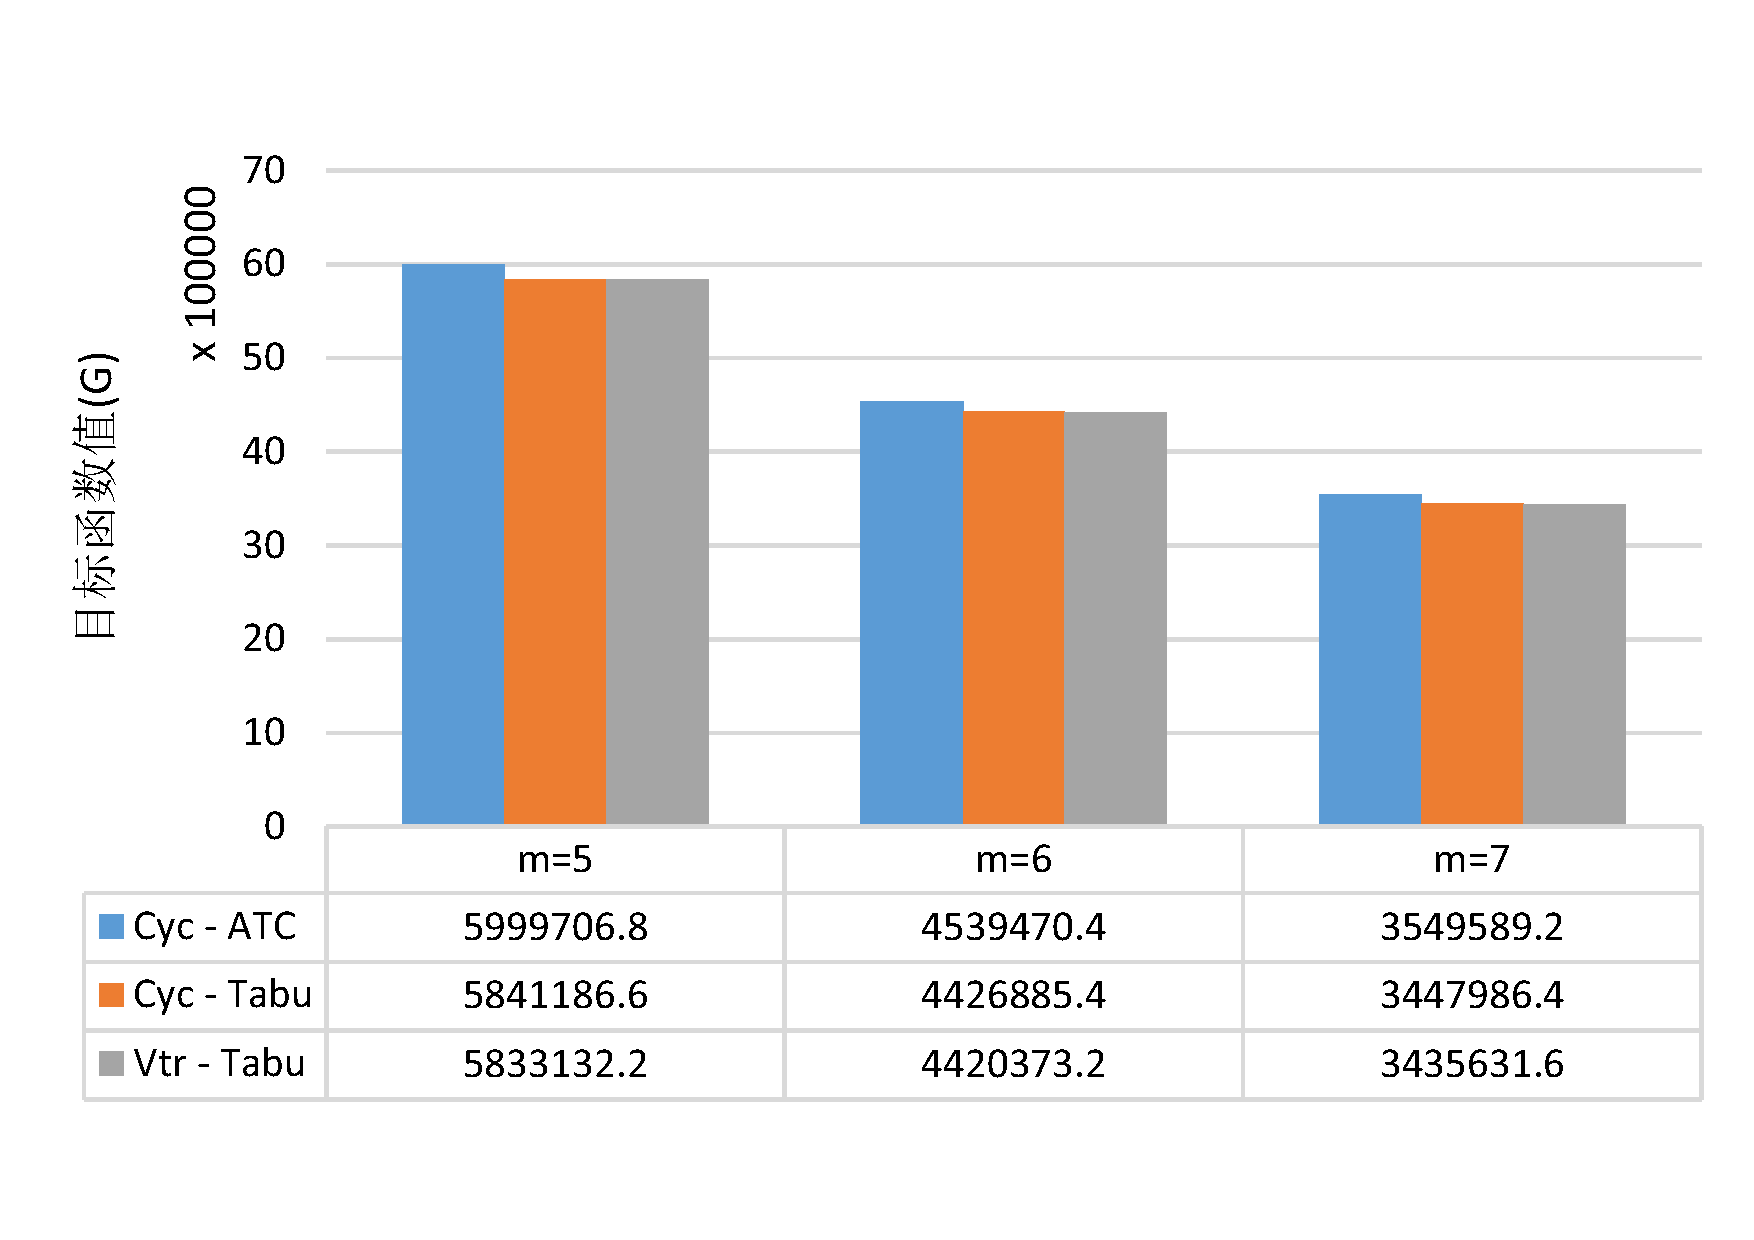
\includegraphics[height = 6cm, angle = -90]{basic_06_750}}
\subfloat[$n = 1000$]{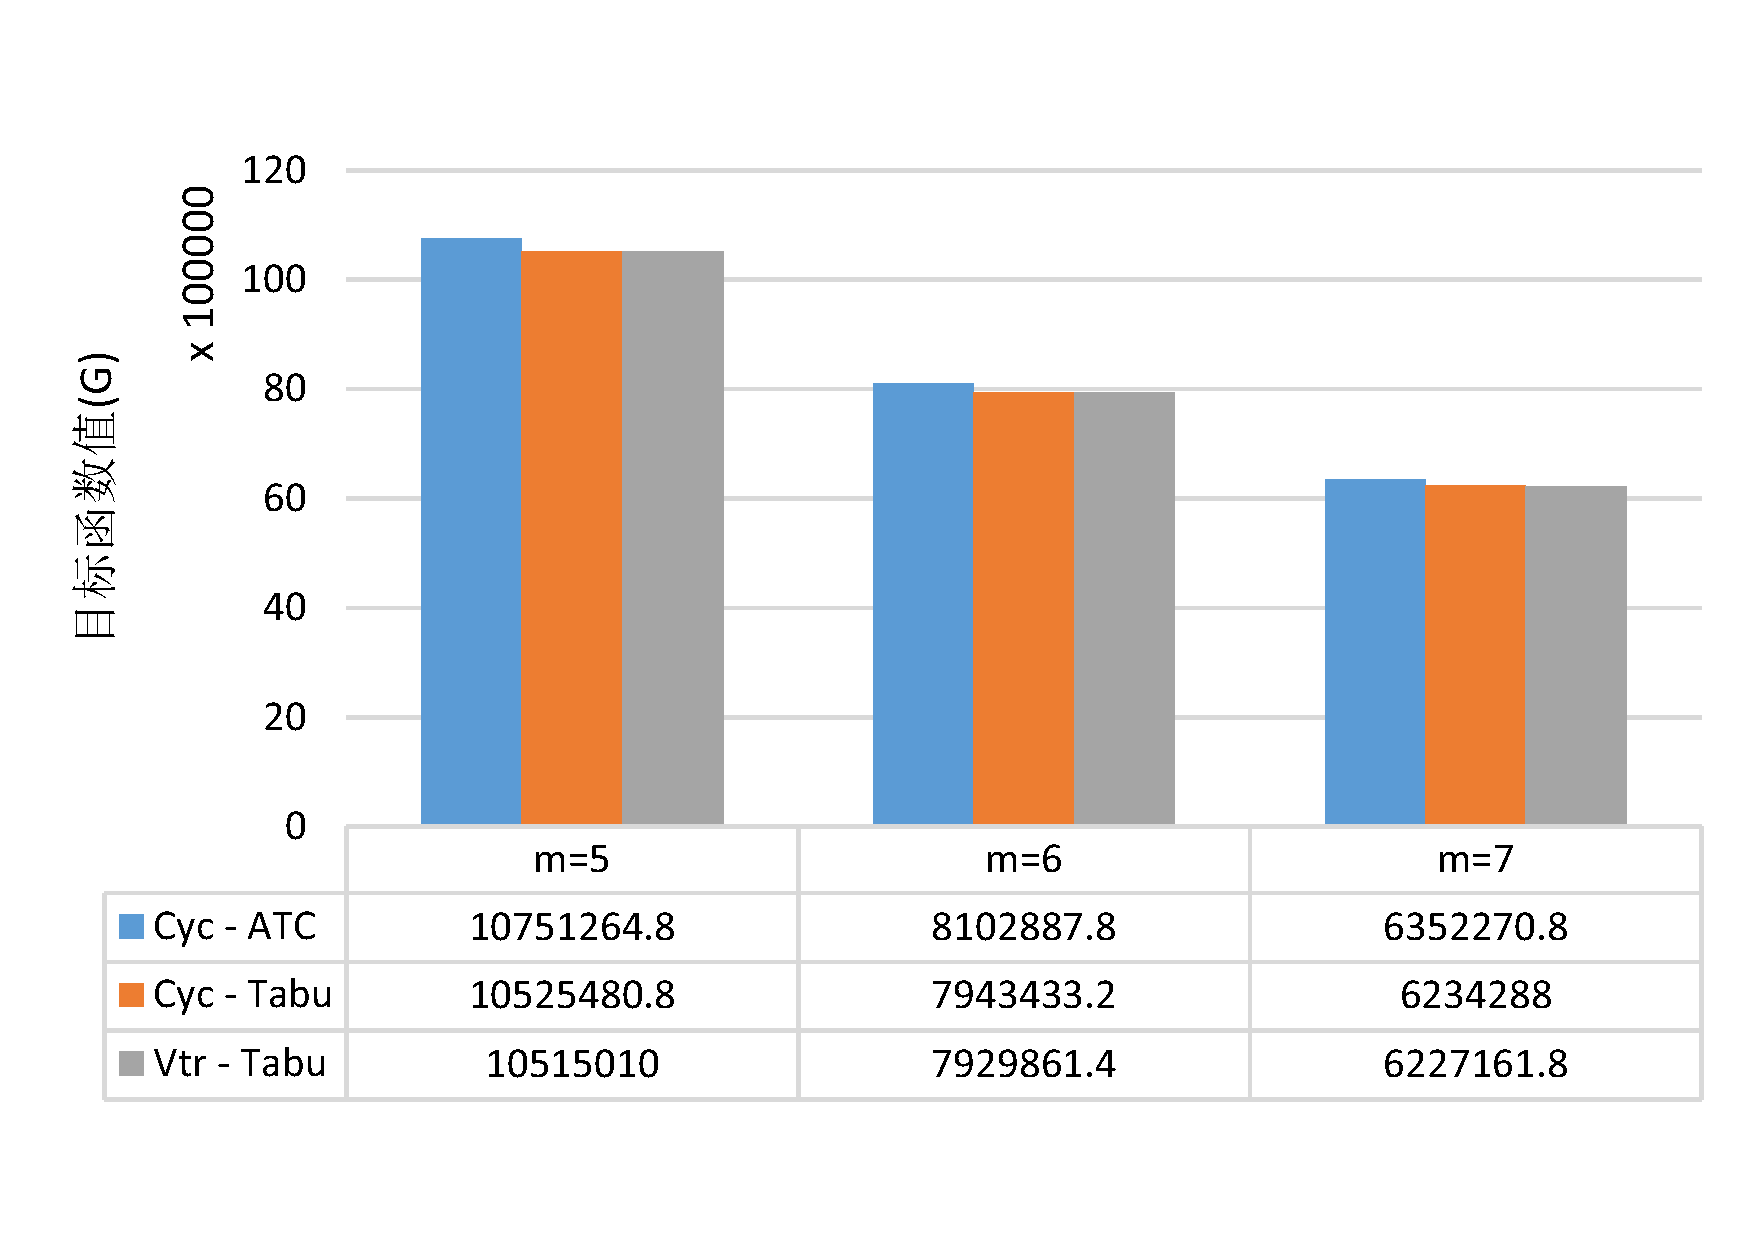
\includegraphics[height = 6cm, angle = -90]{basic_06_1000}}
\caption{\label{fig:result3}模型$1$的Cyc -- ATC、Cyc -- Tabu、Vtr -- Tabu 算法求解目标函数值比较$(\lambda_1 = 0.6)$}
\end{sidewaysfigure}

\begin{sidewaysfigure}
\centering
\subfloat[$n = 20$]{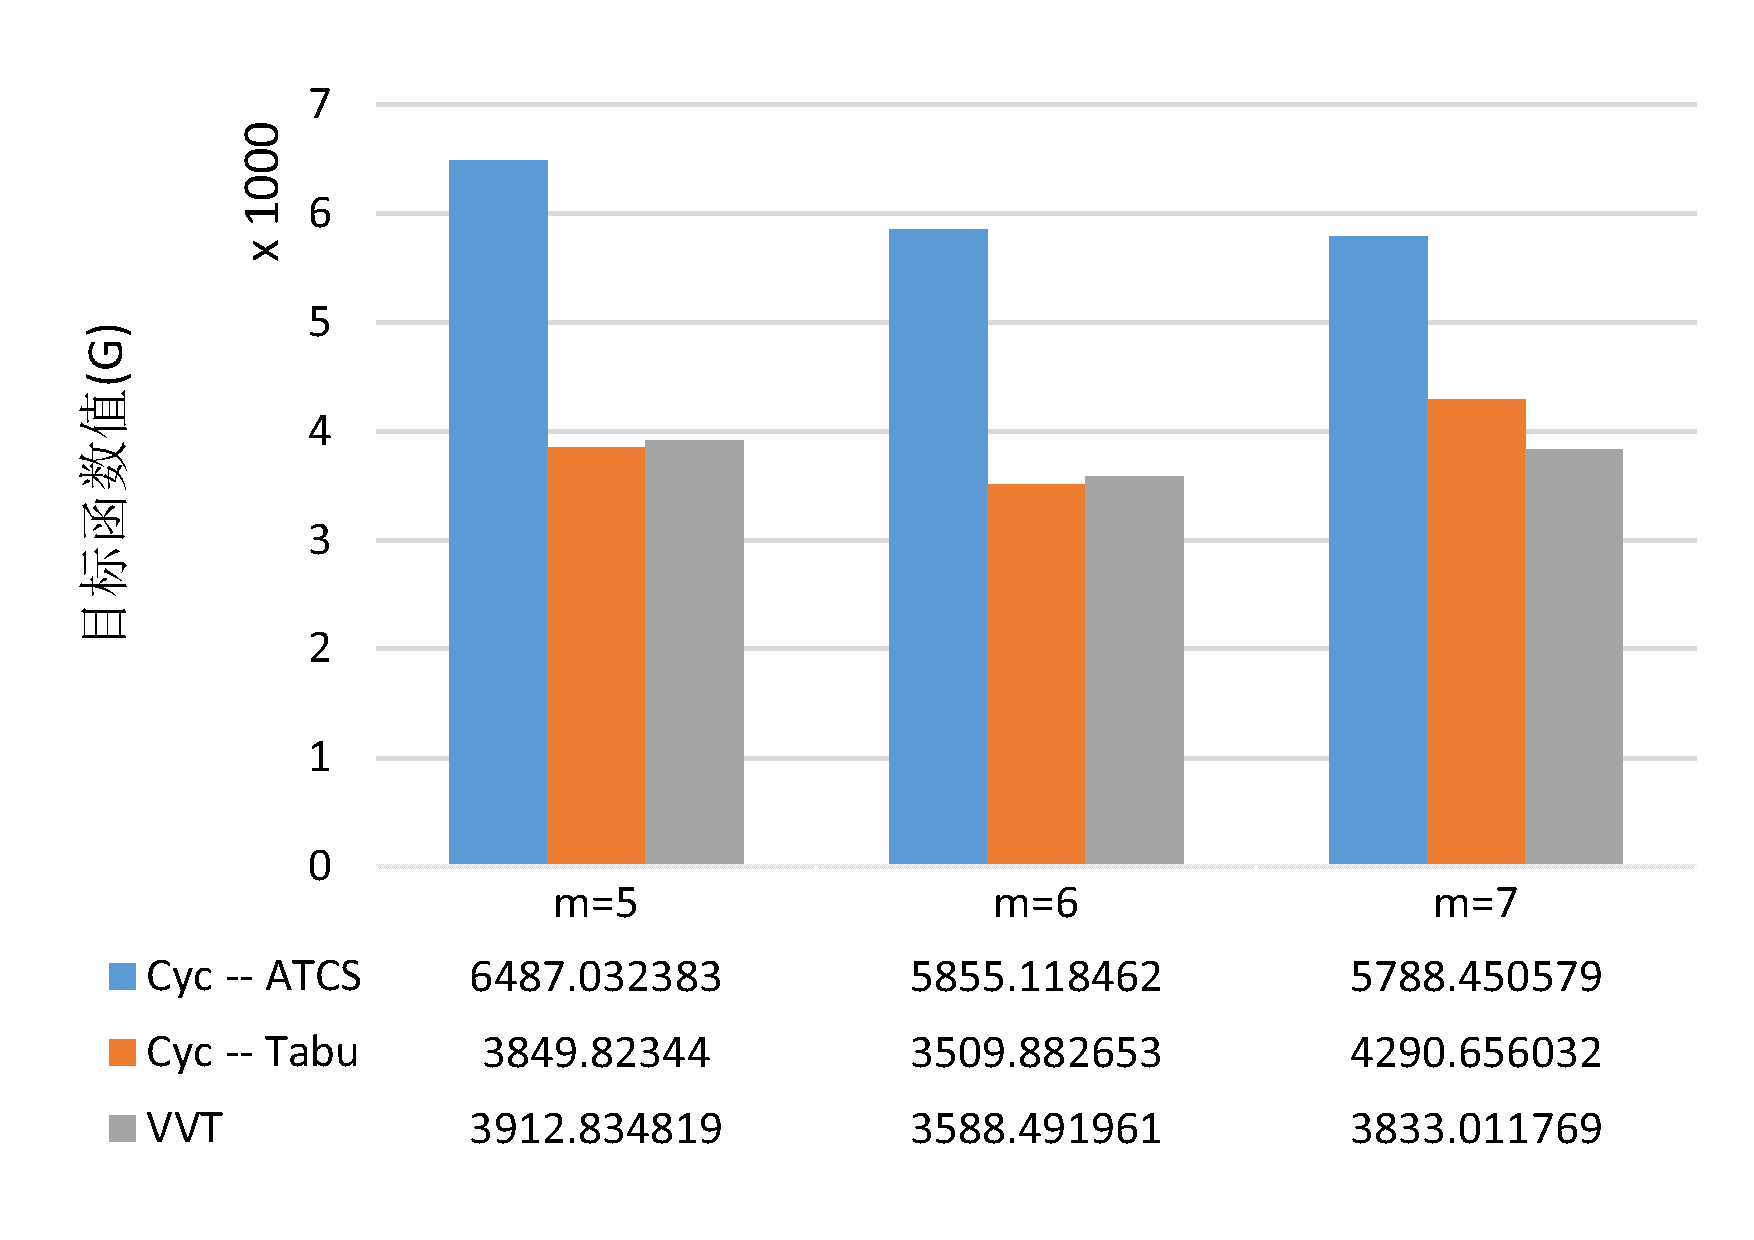
\includegraphics[height = 6cm, angle = -90]{continue_04_20}}
\subfloat[$n = 30$]{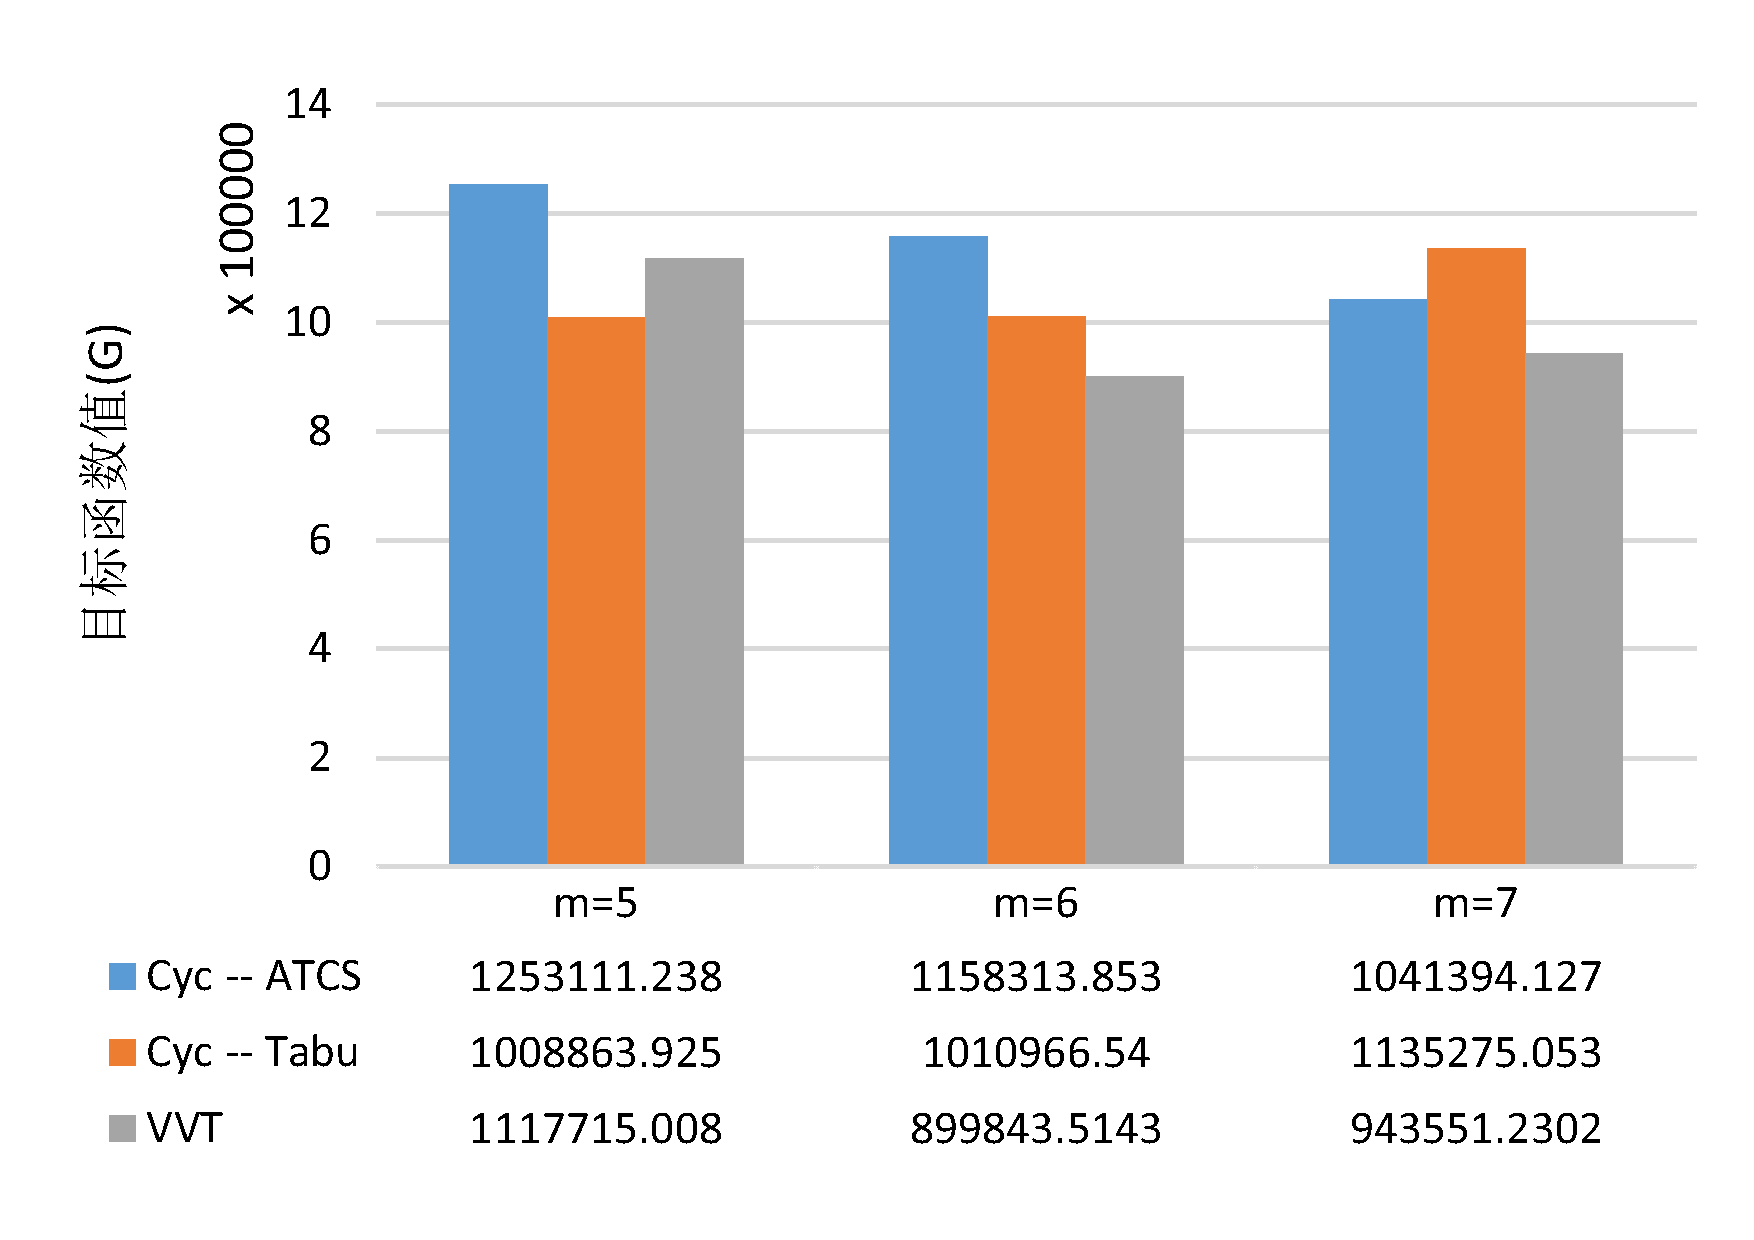
\includegraphics[height = 6cm, angle = -90]{continue_04_300}}
\subfloat[$n = 50$]{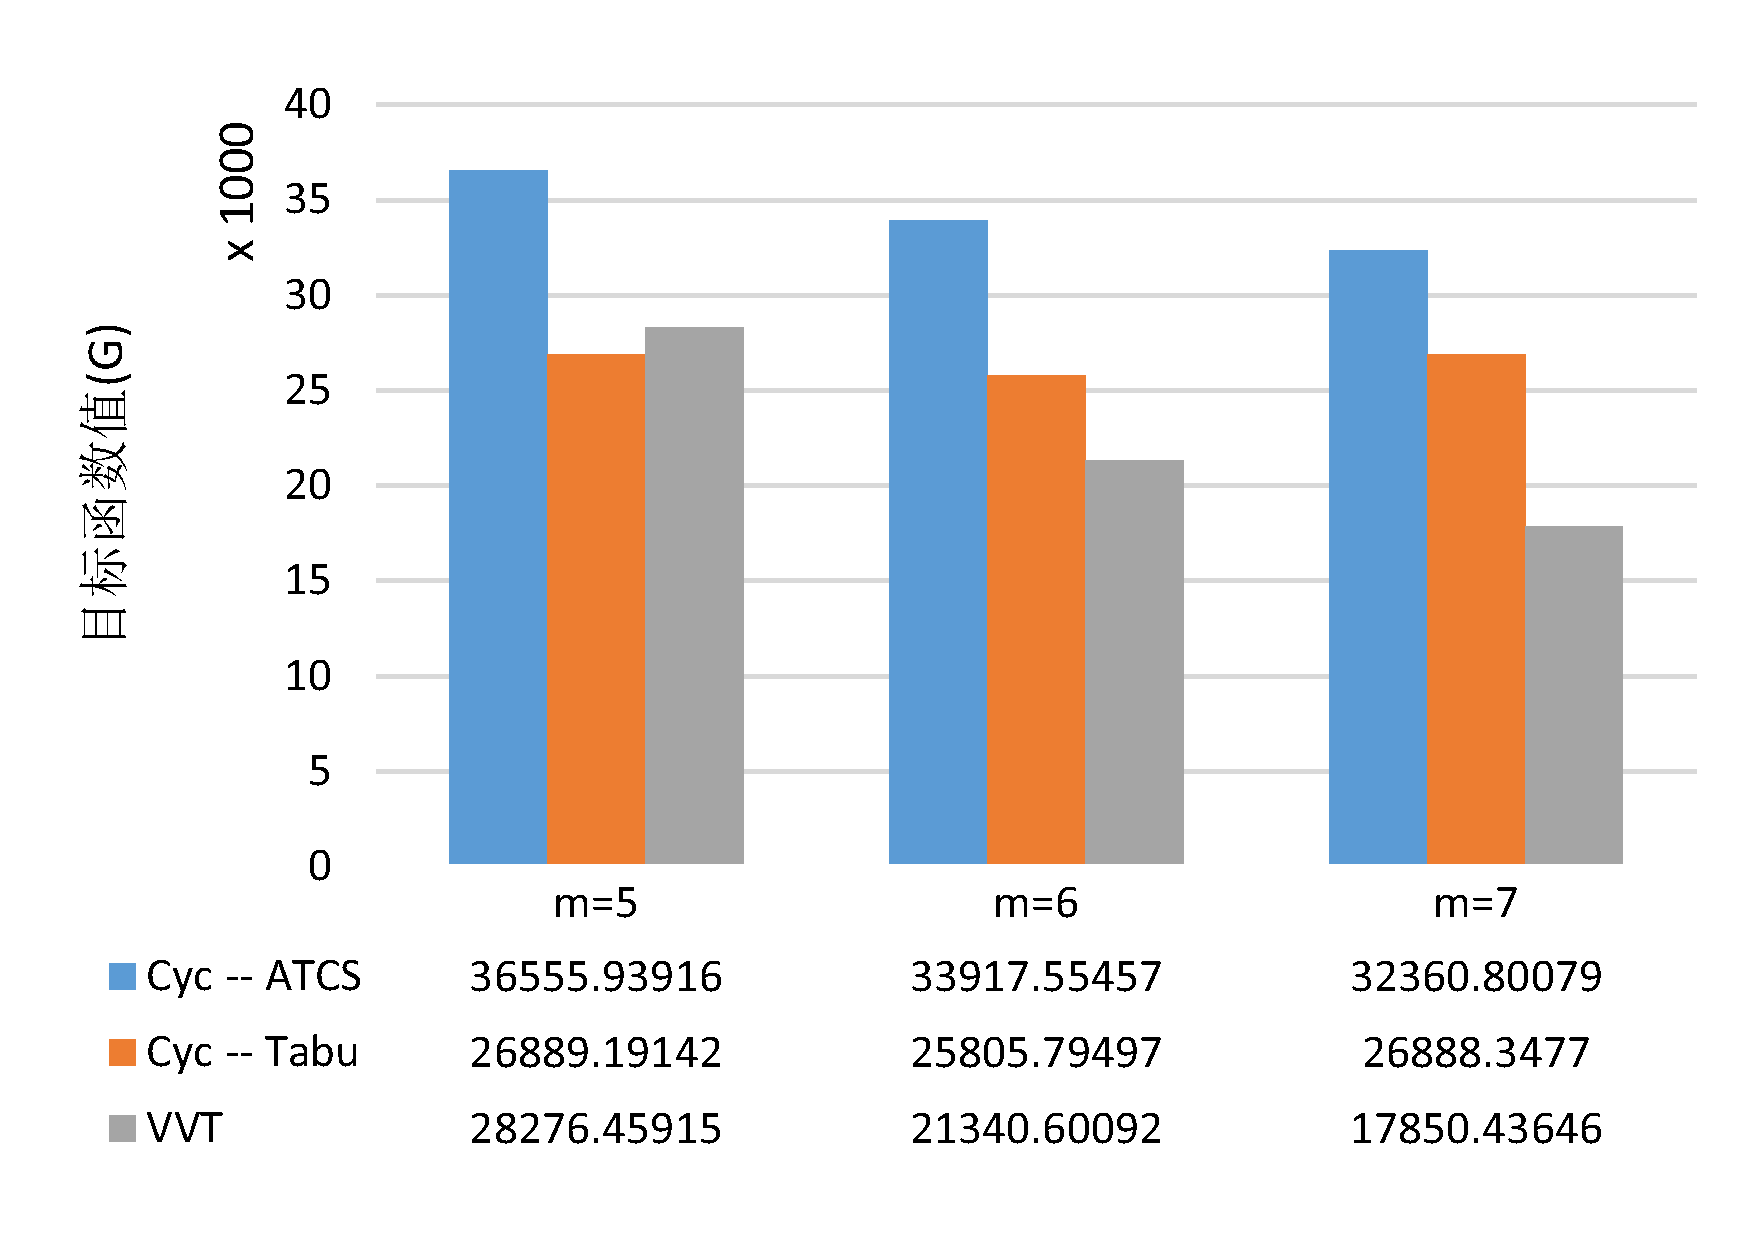
\includegraphics[height = 6cm, angle = -90]{continue_04_50}}
\subfloat[$n = 70$]{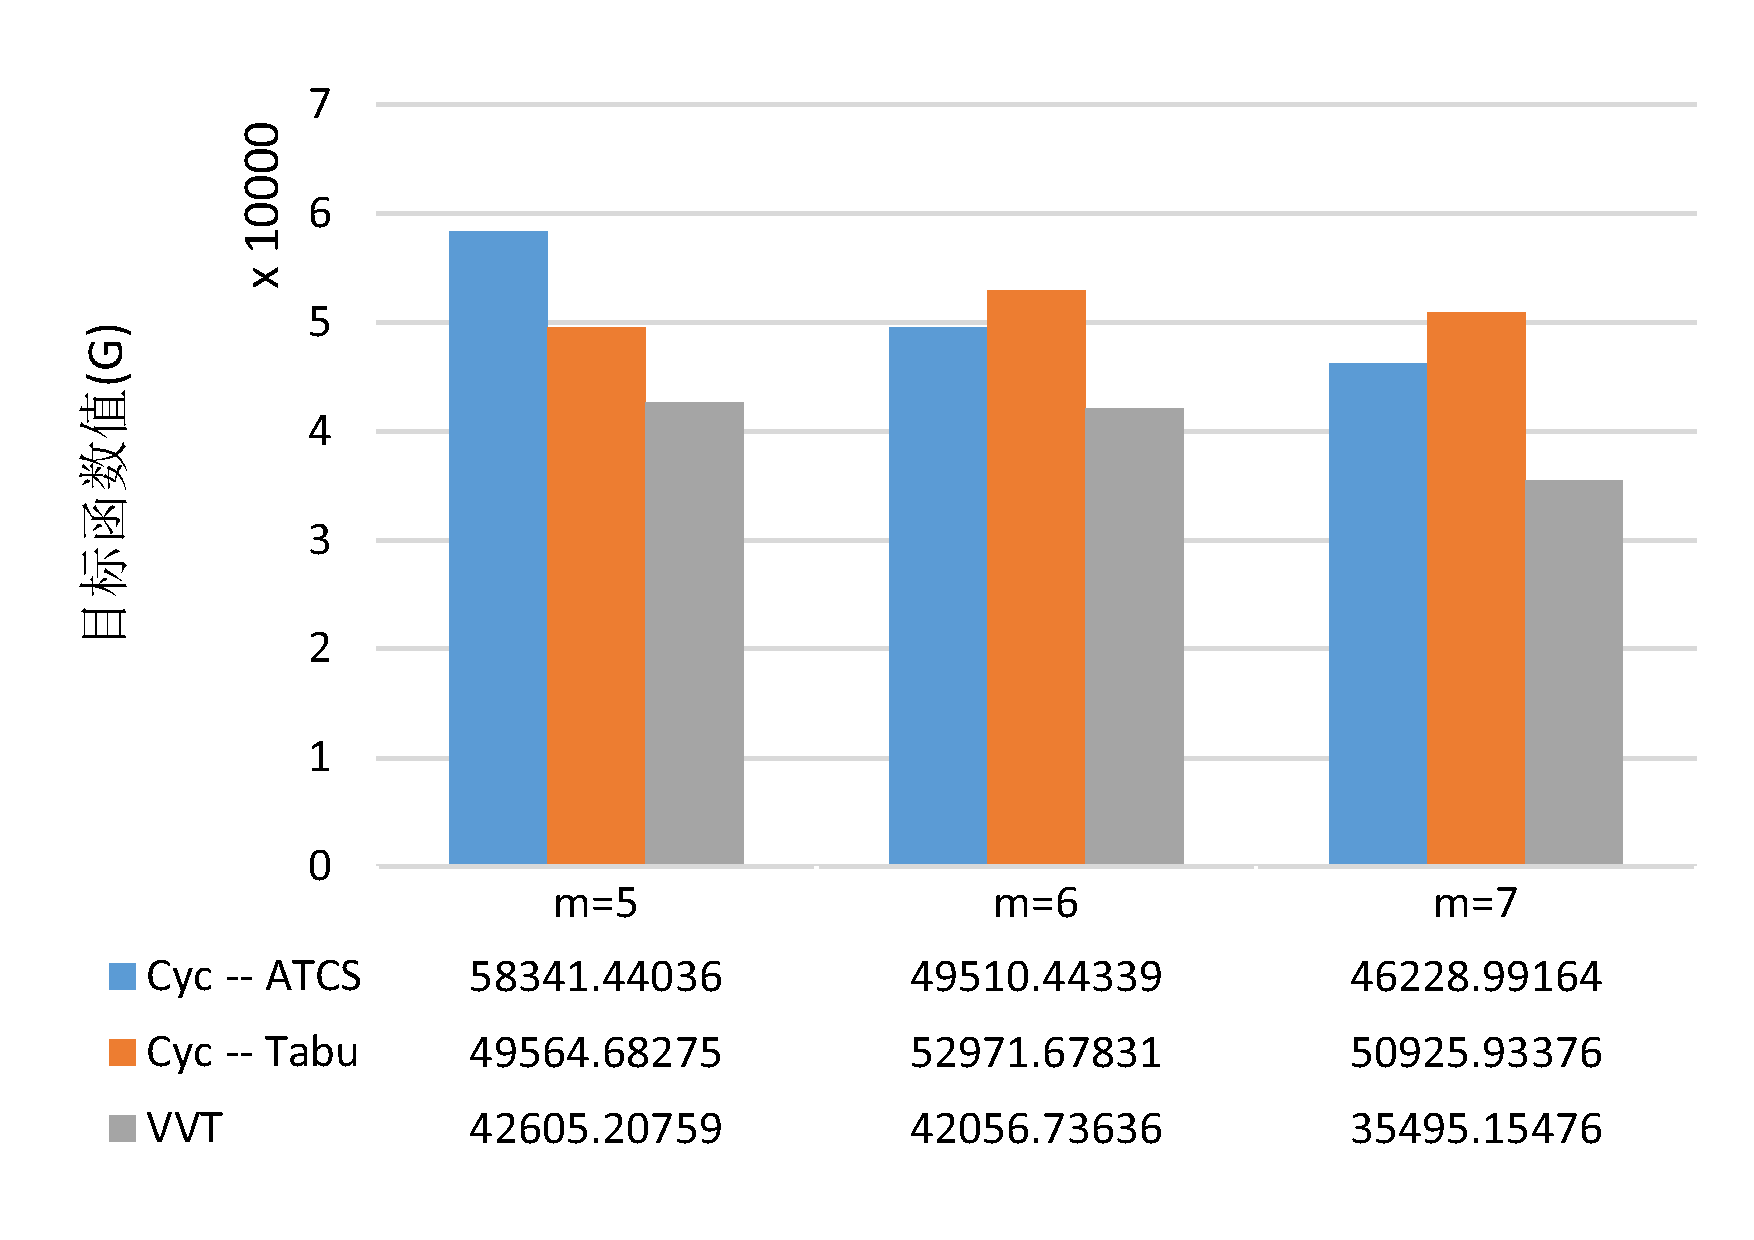
\includegraphics[height = 6cm, angle = -90]{continue_04_70}}\\
\subfloat[$n = 100$]{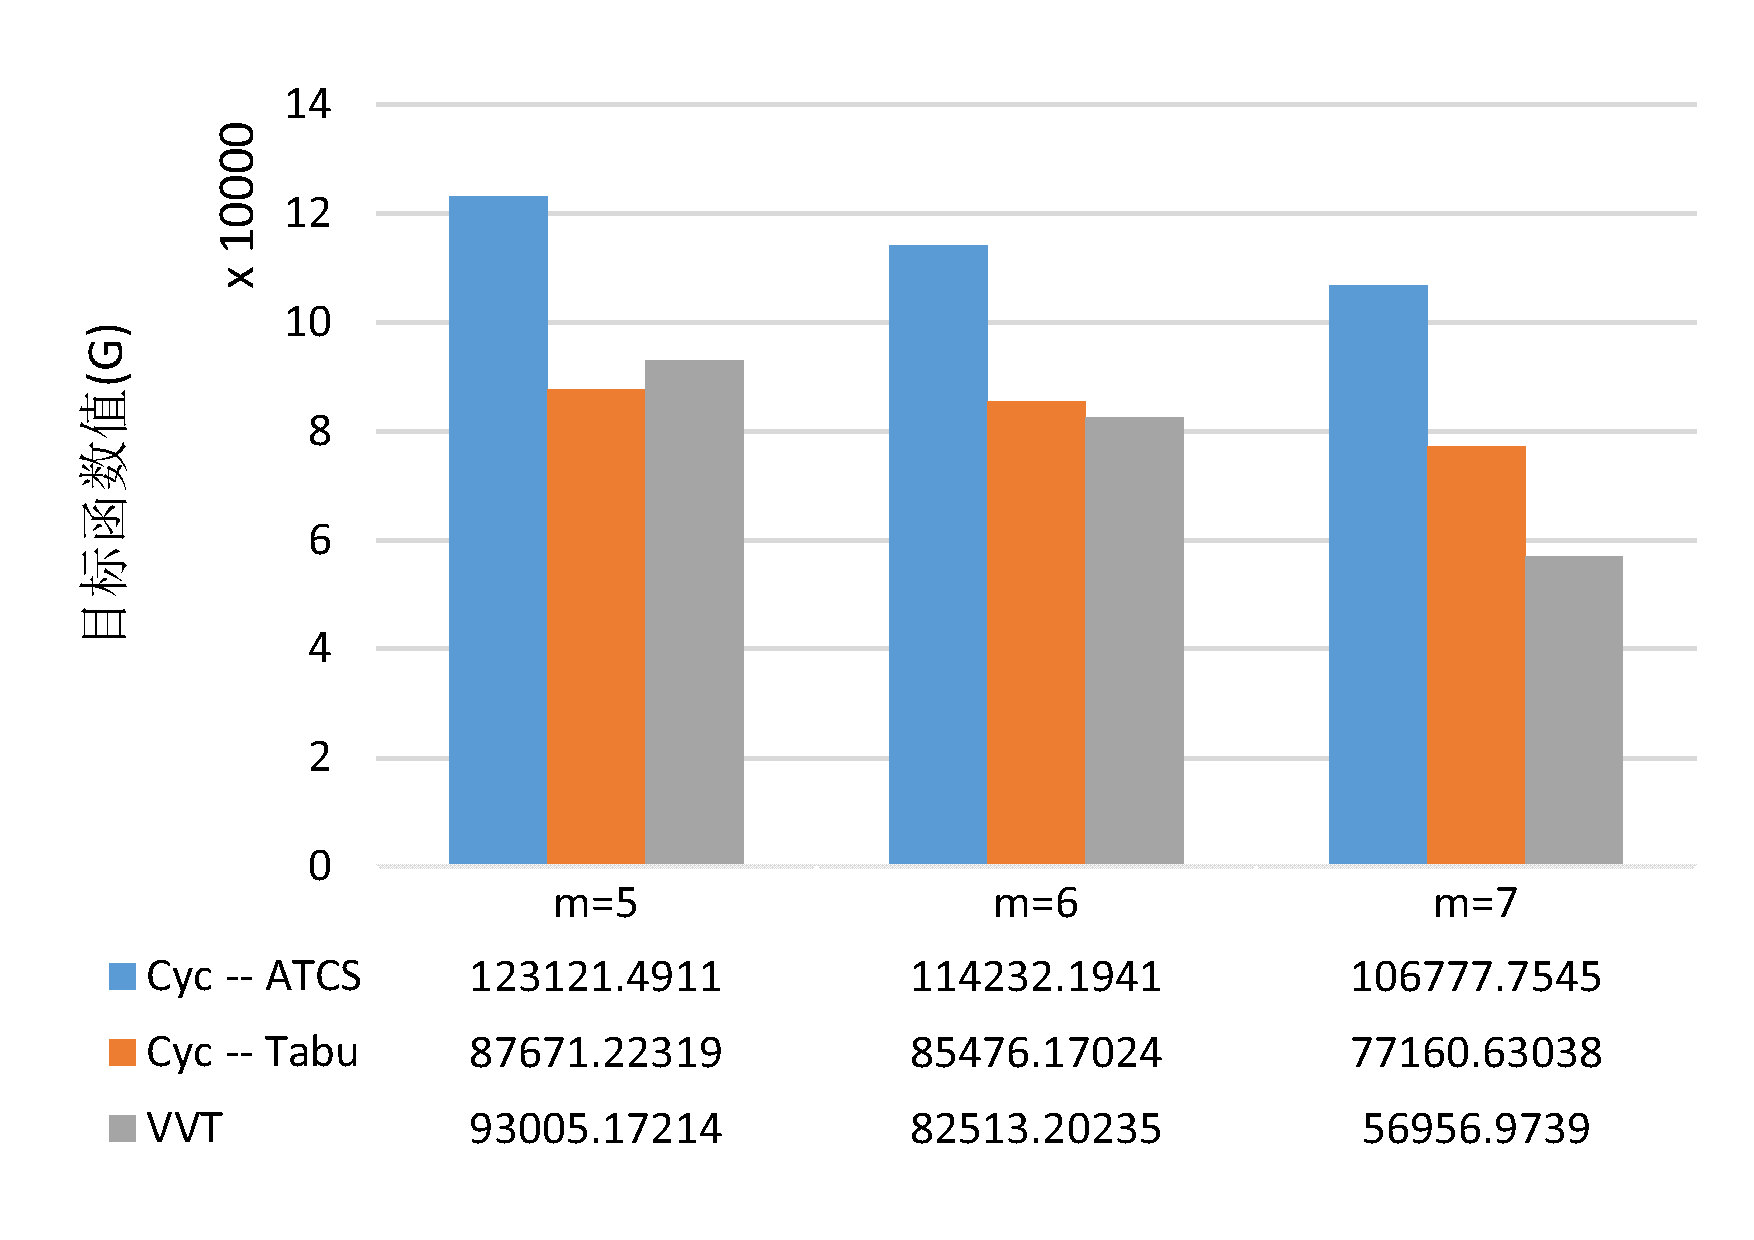
\includegraphics[height = 6cm, angle = -90]{continue_04_100}}
\subfloat[$n = 150$]{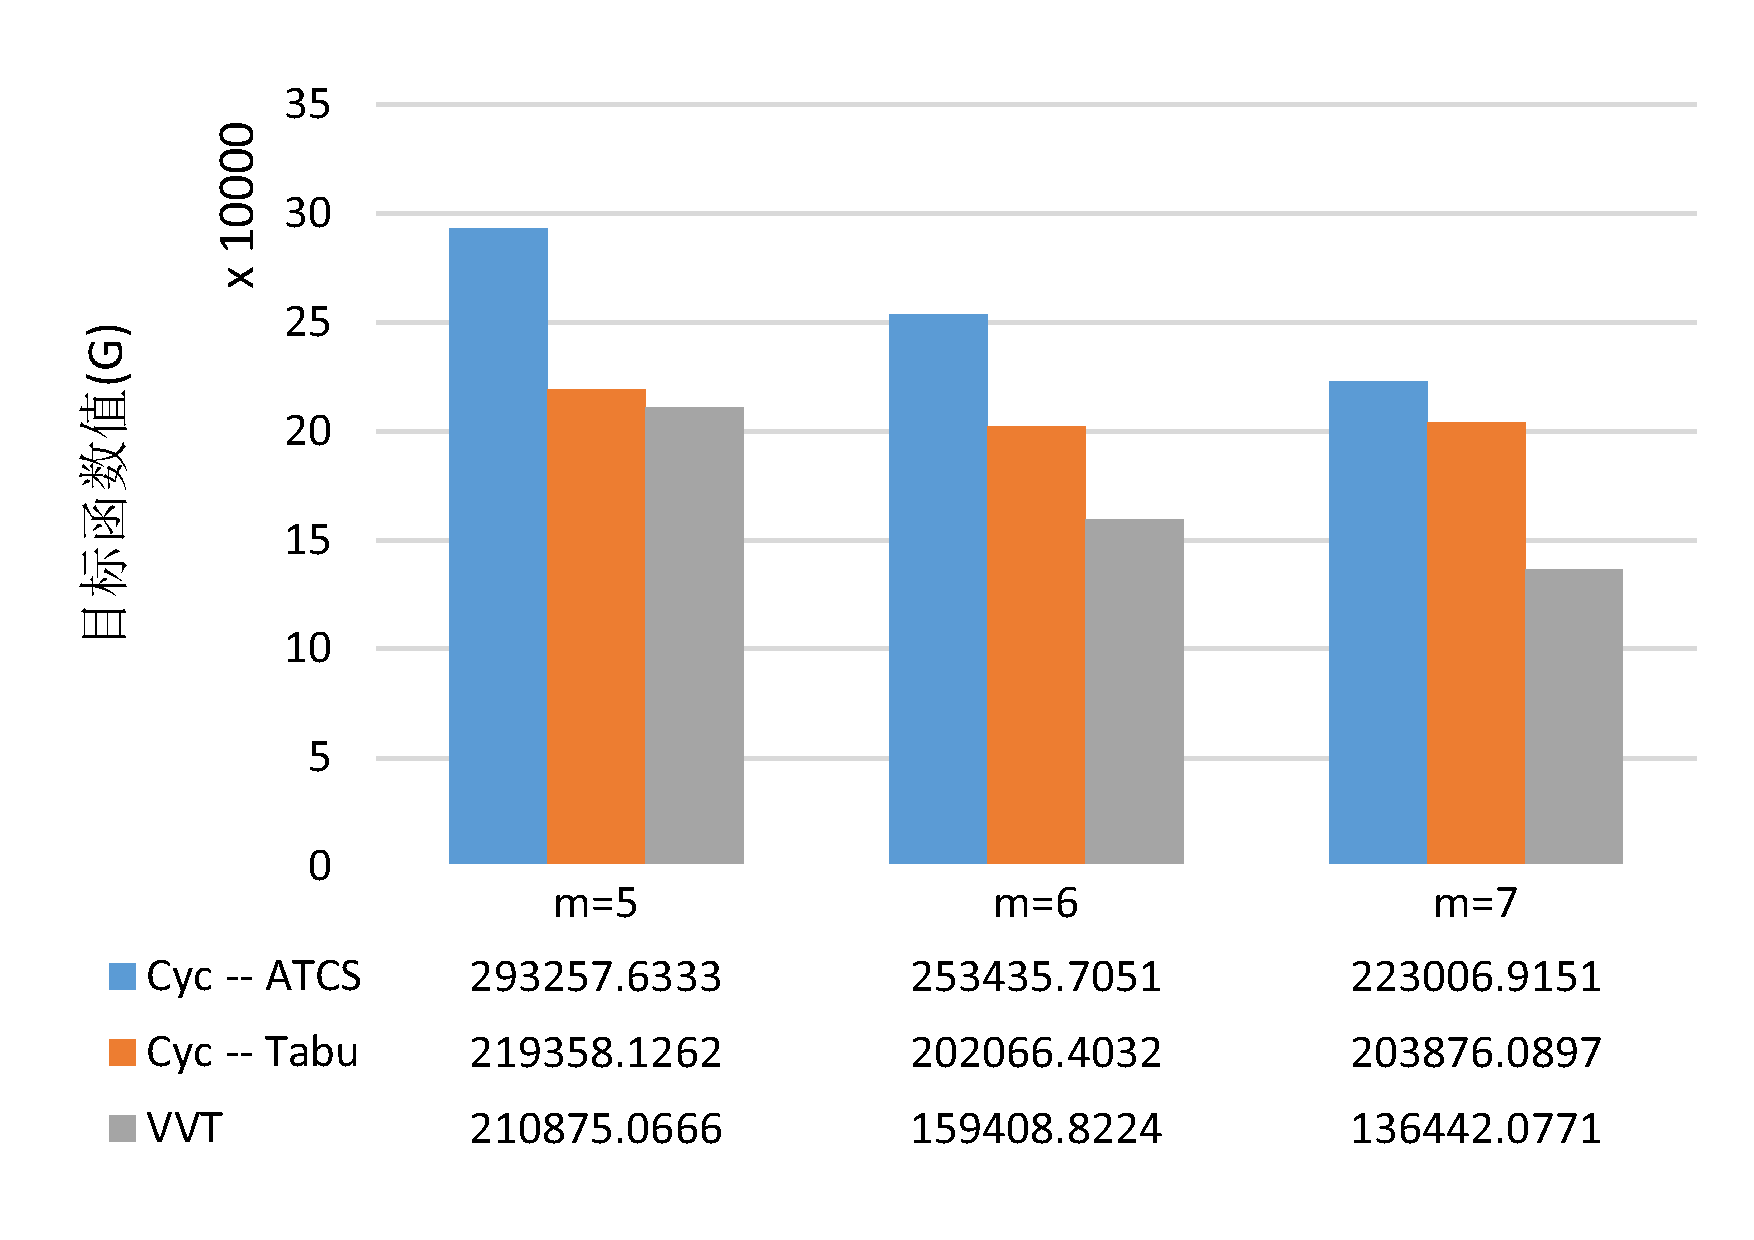
\includegraphics[height = 6cm, angle = -90]{continue_04_150}}
\subfloat[$n = 200$]{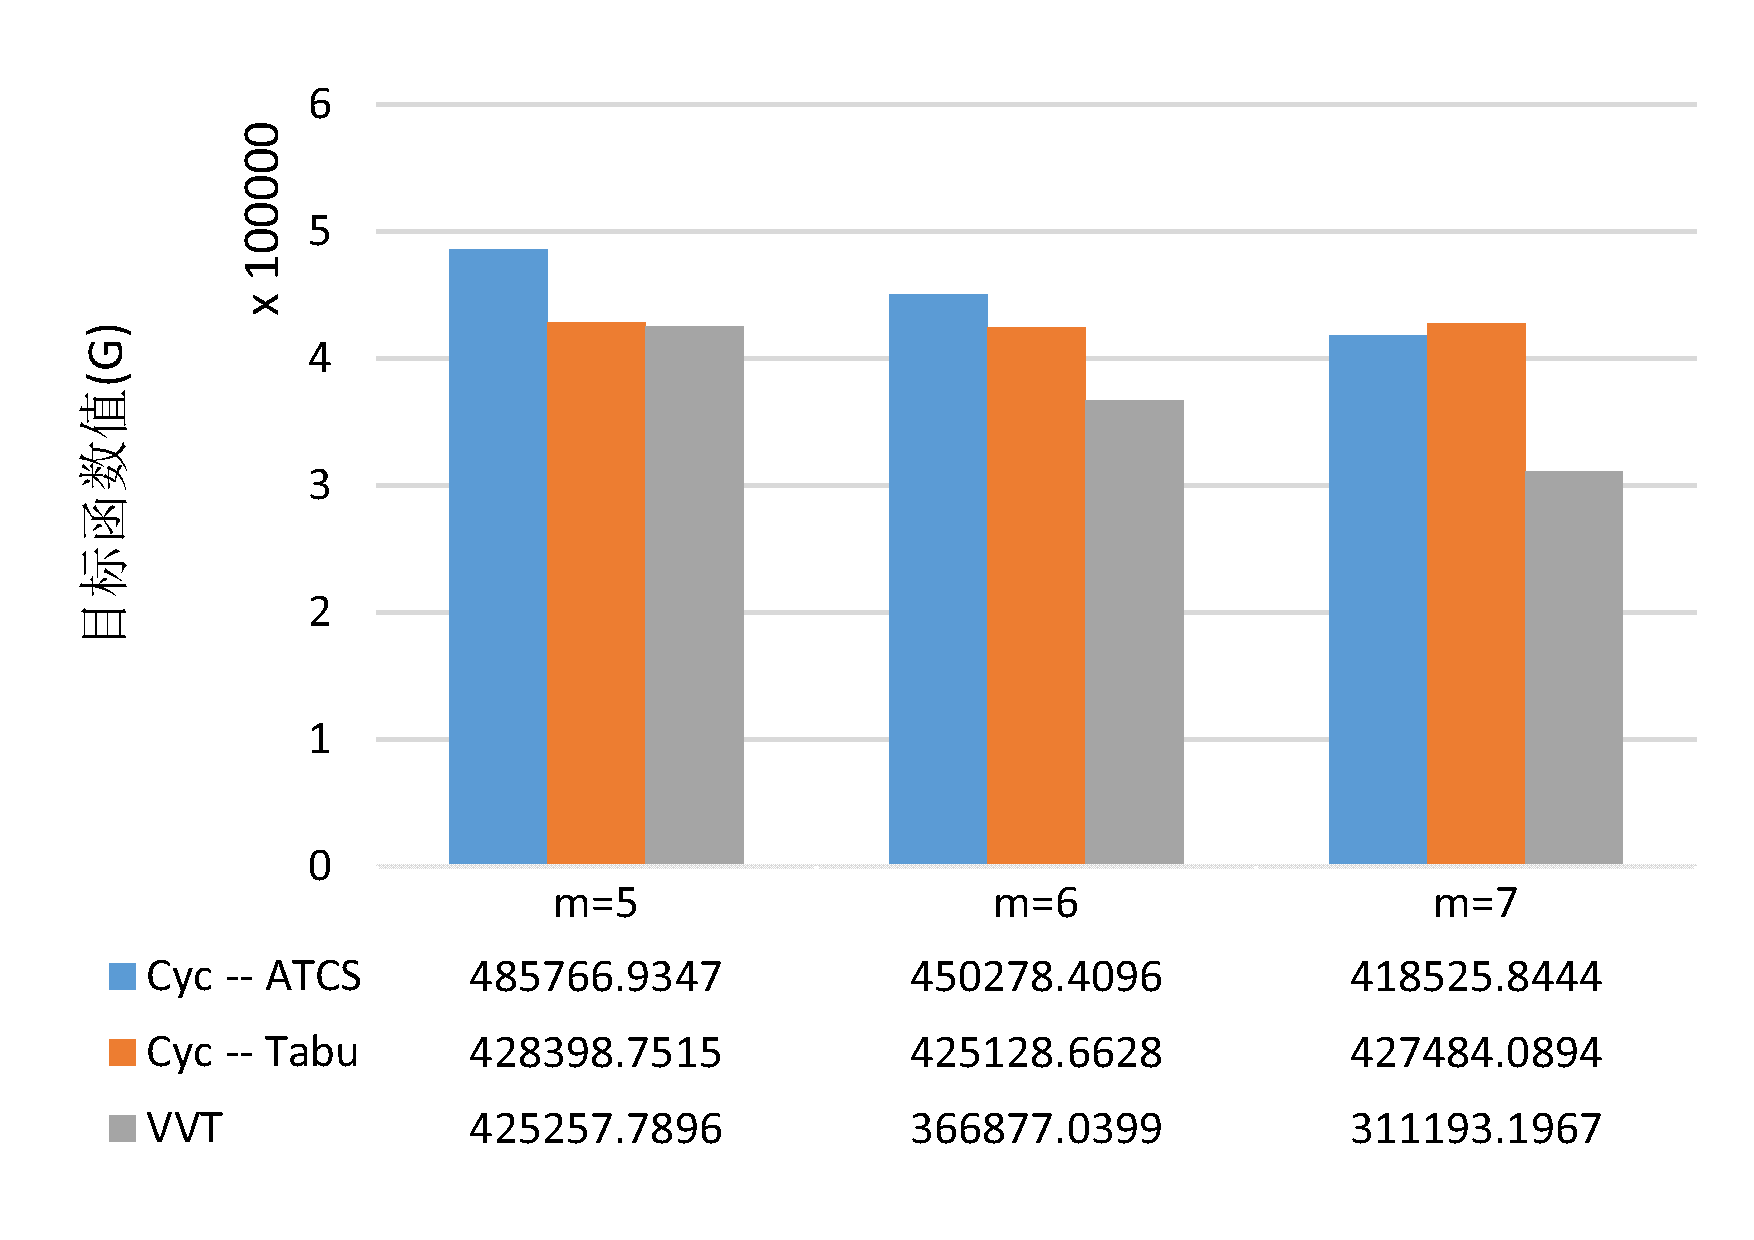
\includegraphics[height = 6cm, angle = -90]{continue_04_200}}
\subfloat[$n = 300$]{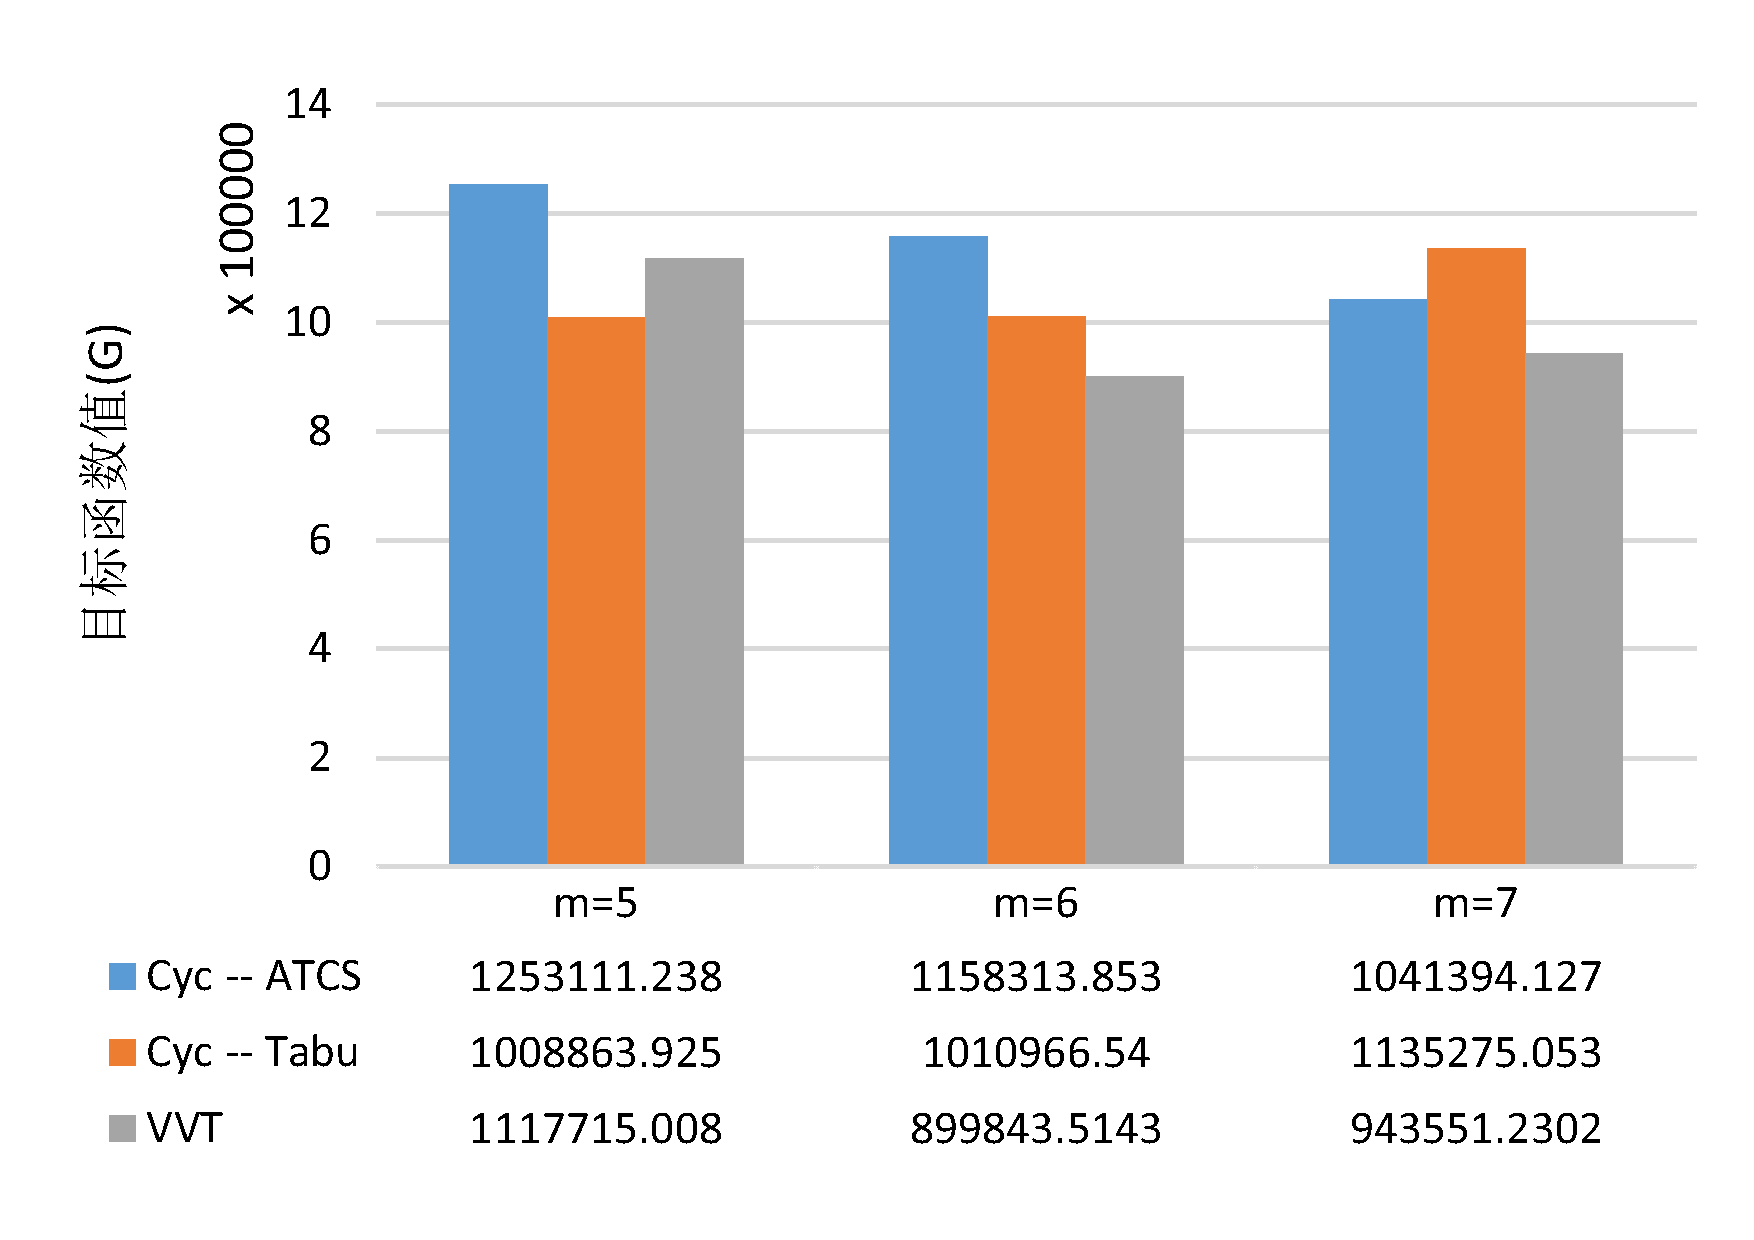
\includegraphics[height = 6cm, angle = -90]{continue_04_300}}\\
\subfloat[$n = 500$]{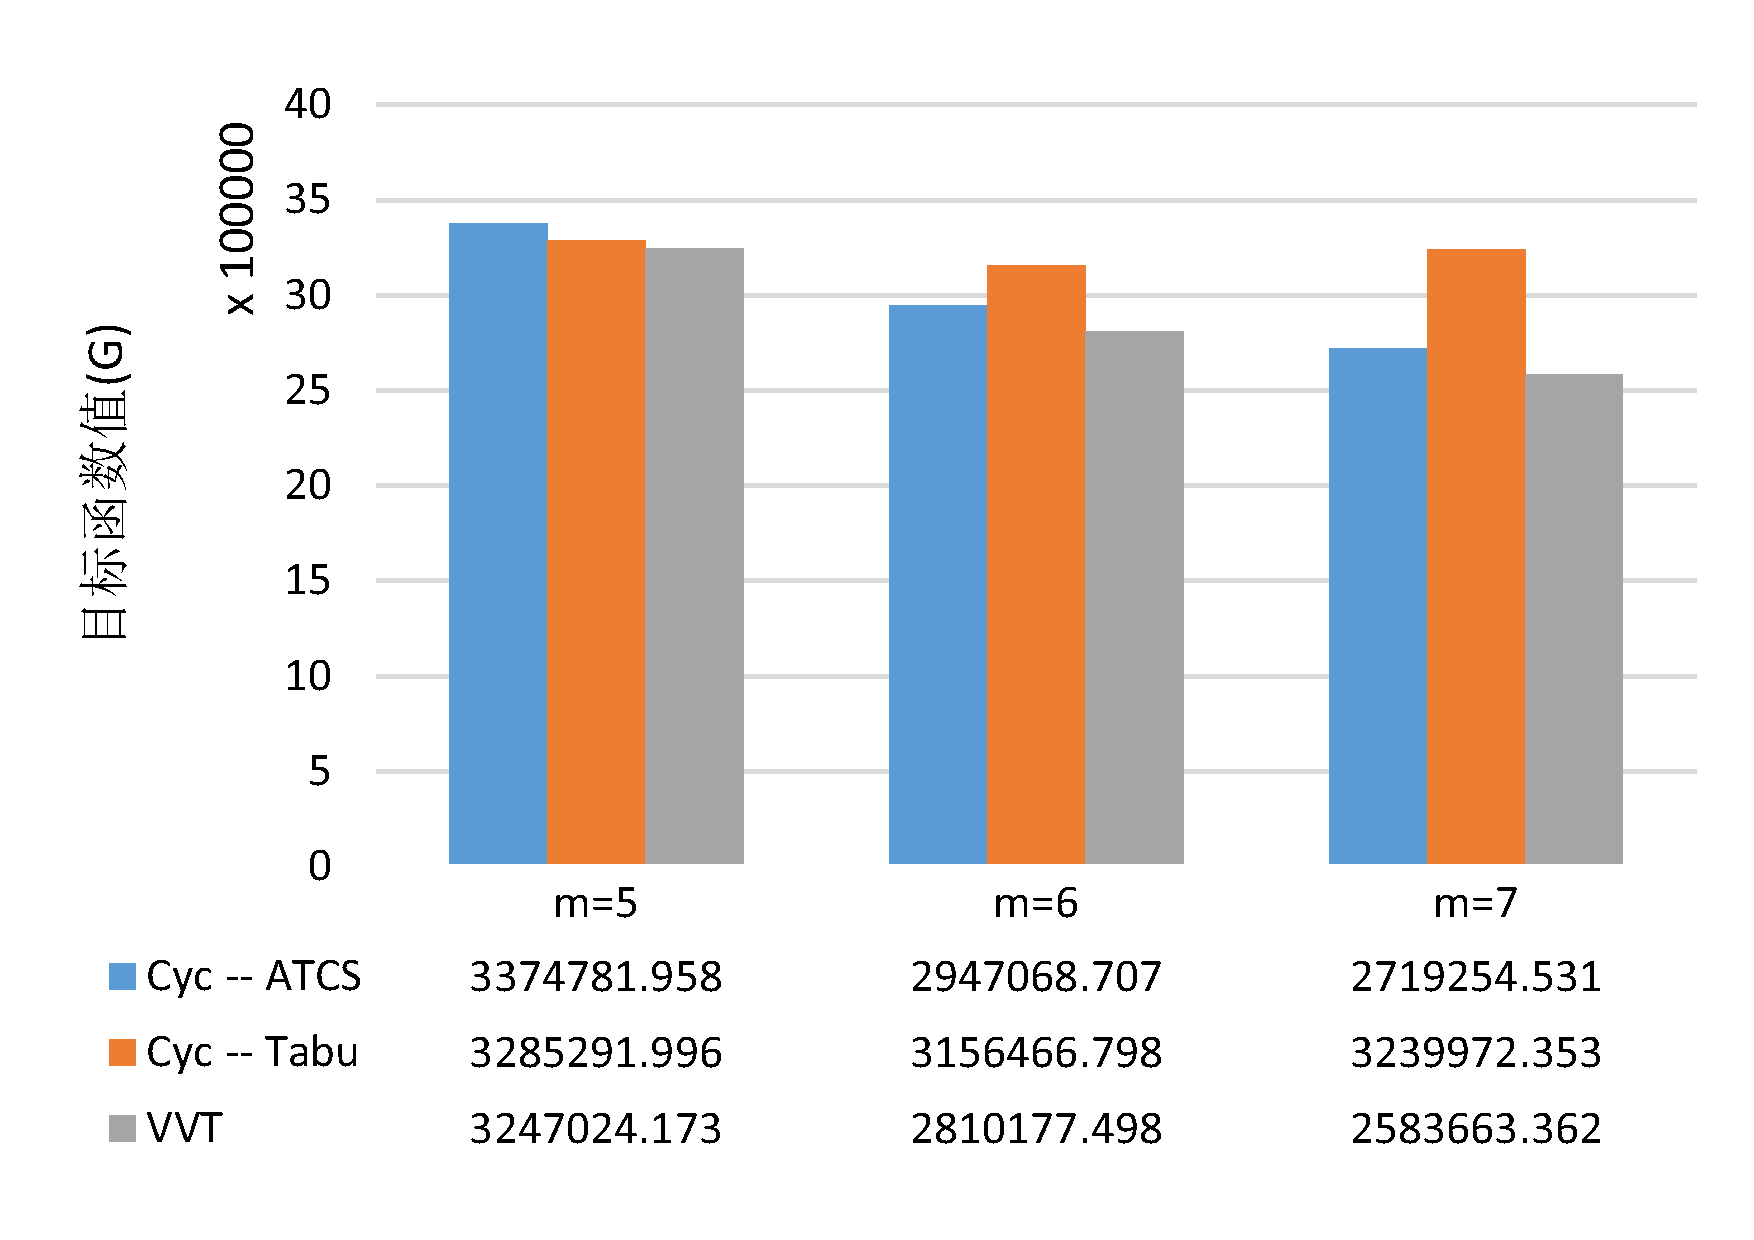
\includegraphics[height = 6cm, angle = -90]{continue_04_500}}
\subfloat[$n = 750$]{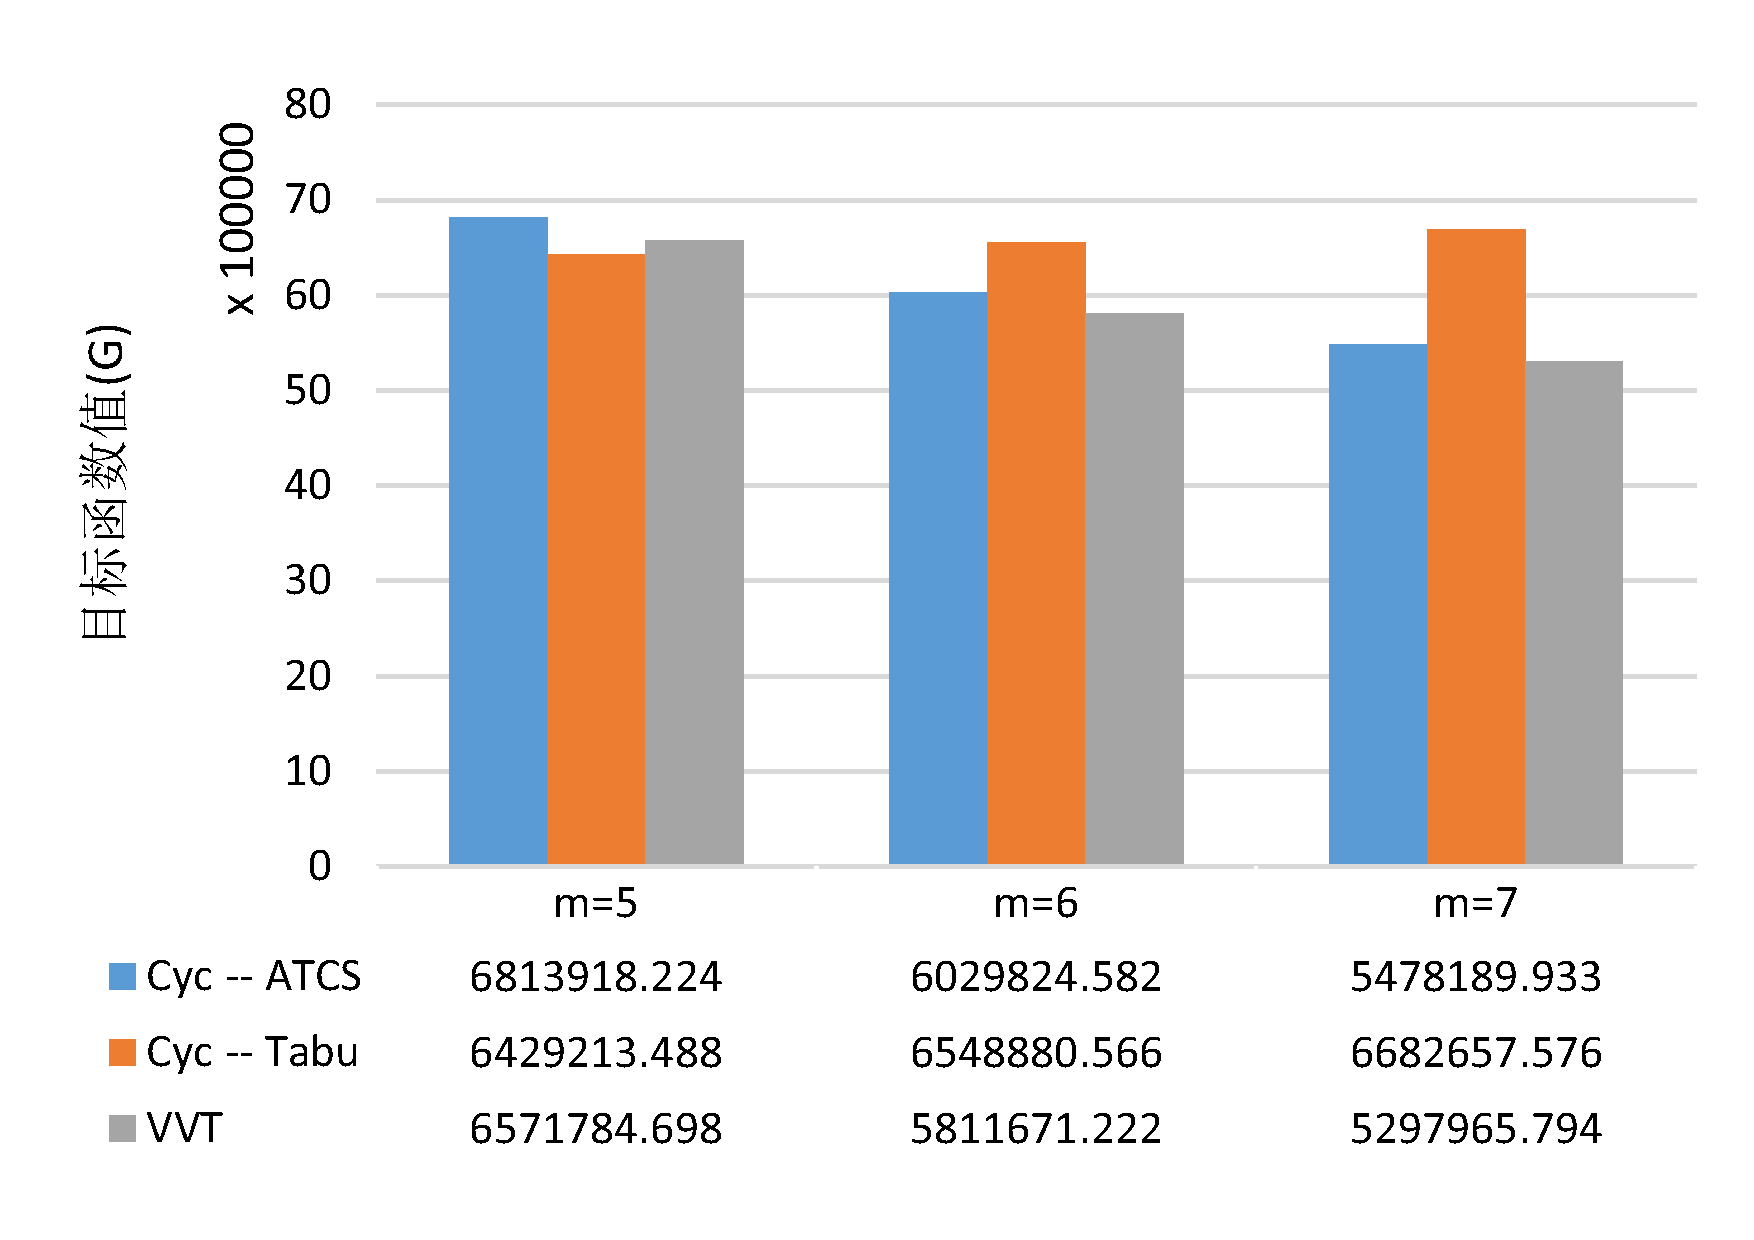
\includegraphics[height = 6cm, angle = -90]{continue_04_750}}
\subfloat[$n = 1000$]{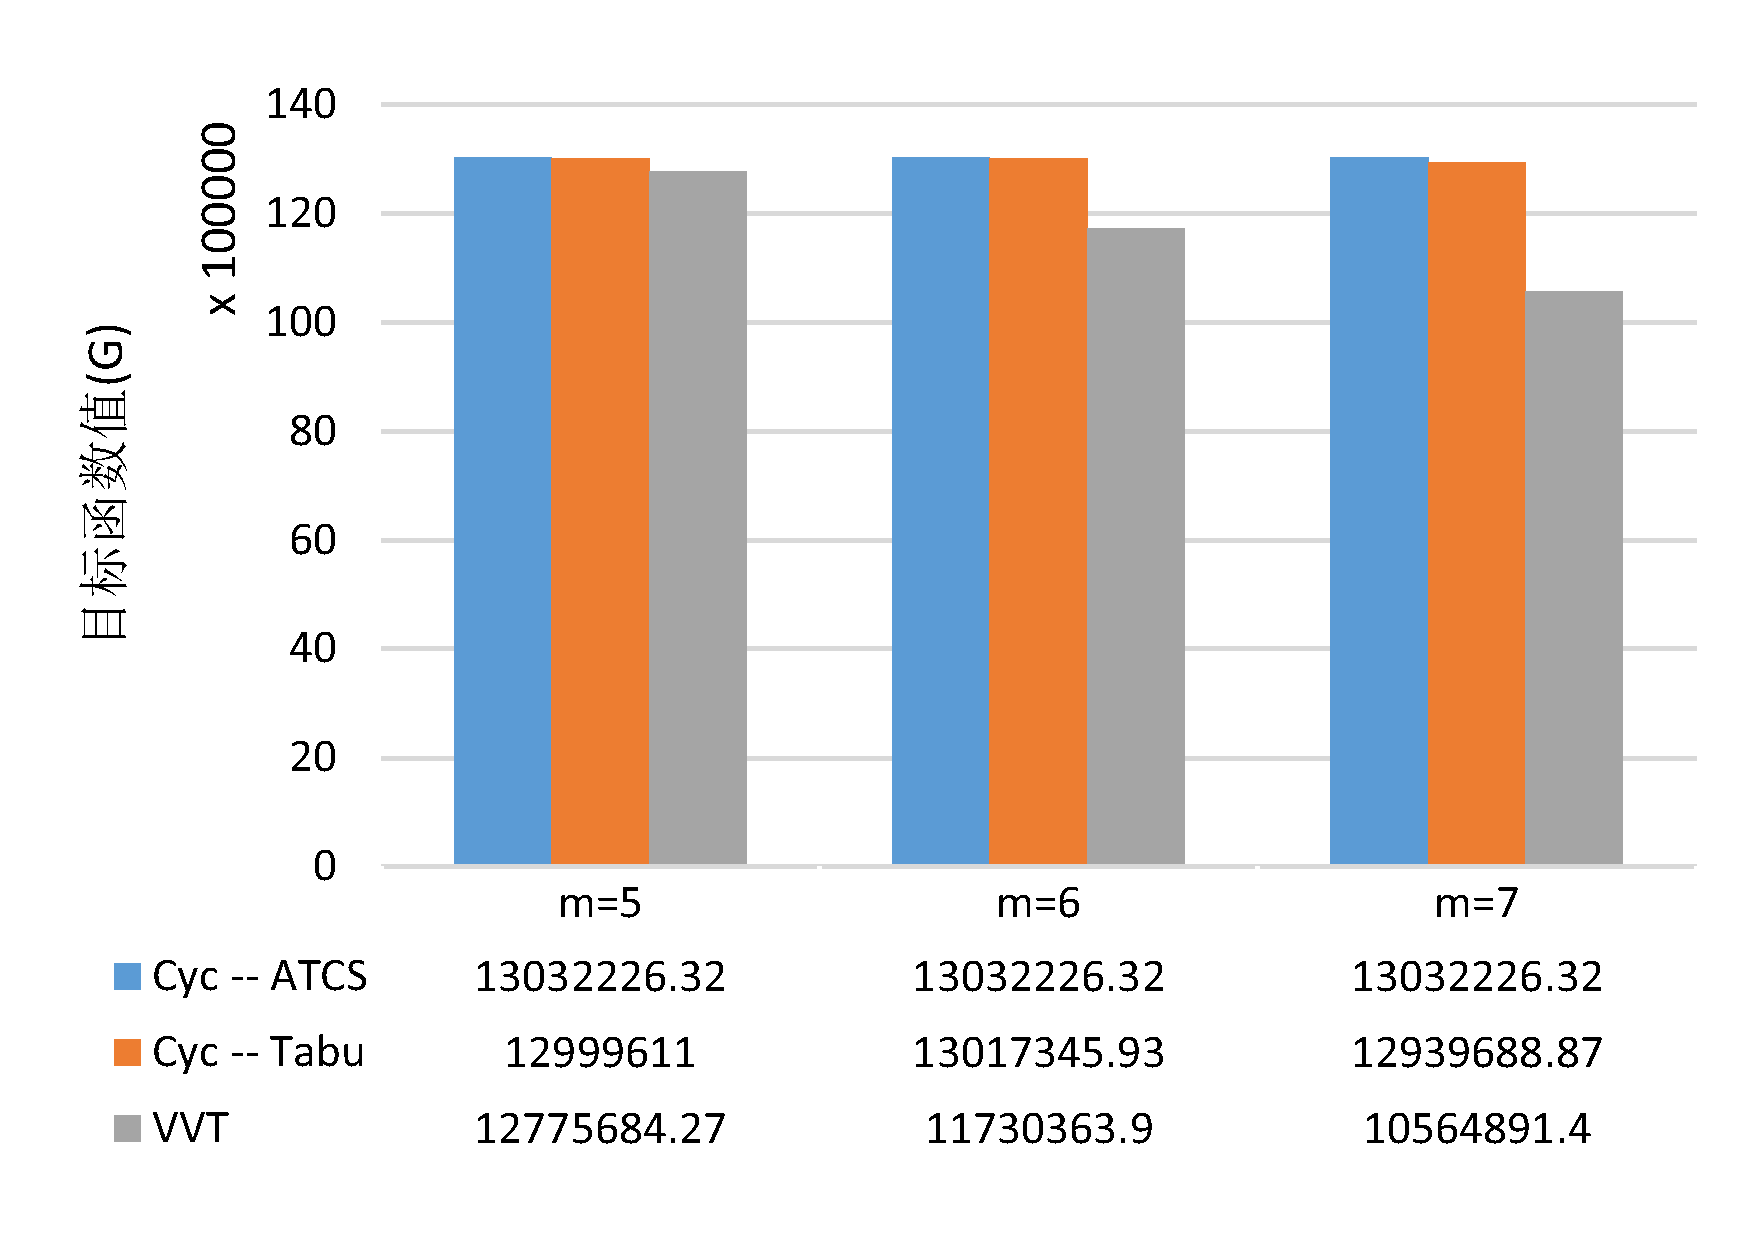
\includegraphics[height = 6cm, angle = -90]{continue_04_1000}}
\caption{\label{fig:result4}模型$2$的Cyc -- ATCS、Cyc -- Tabu、VVT 算法求解目标函数值比较$(\lambda_1 = 0.4)$}
\end{sidewaysfigure}

\begin{sidewaysfigure}
\centering
\subfloat[$n = 20$]{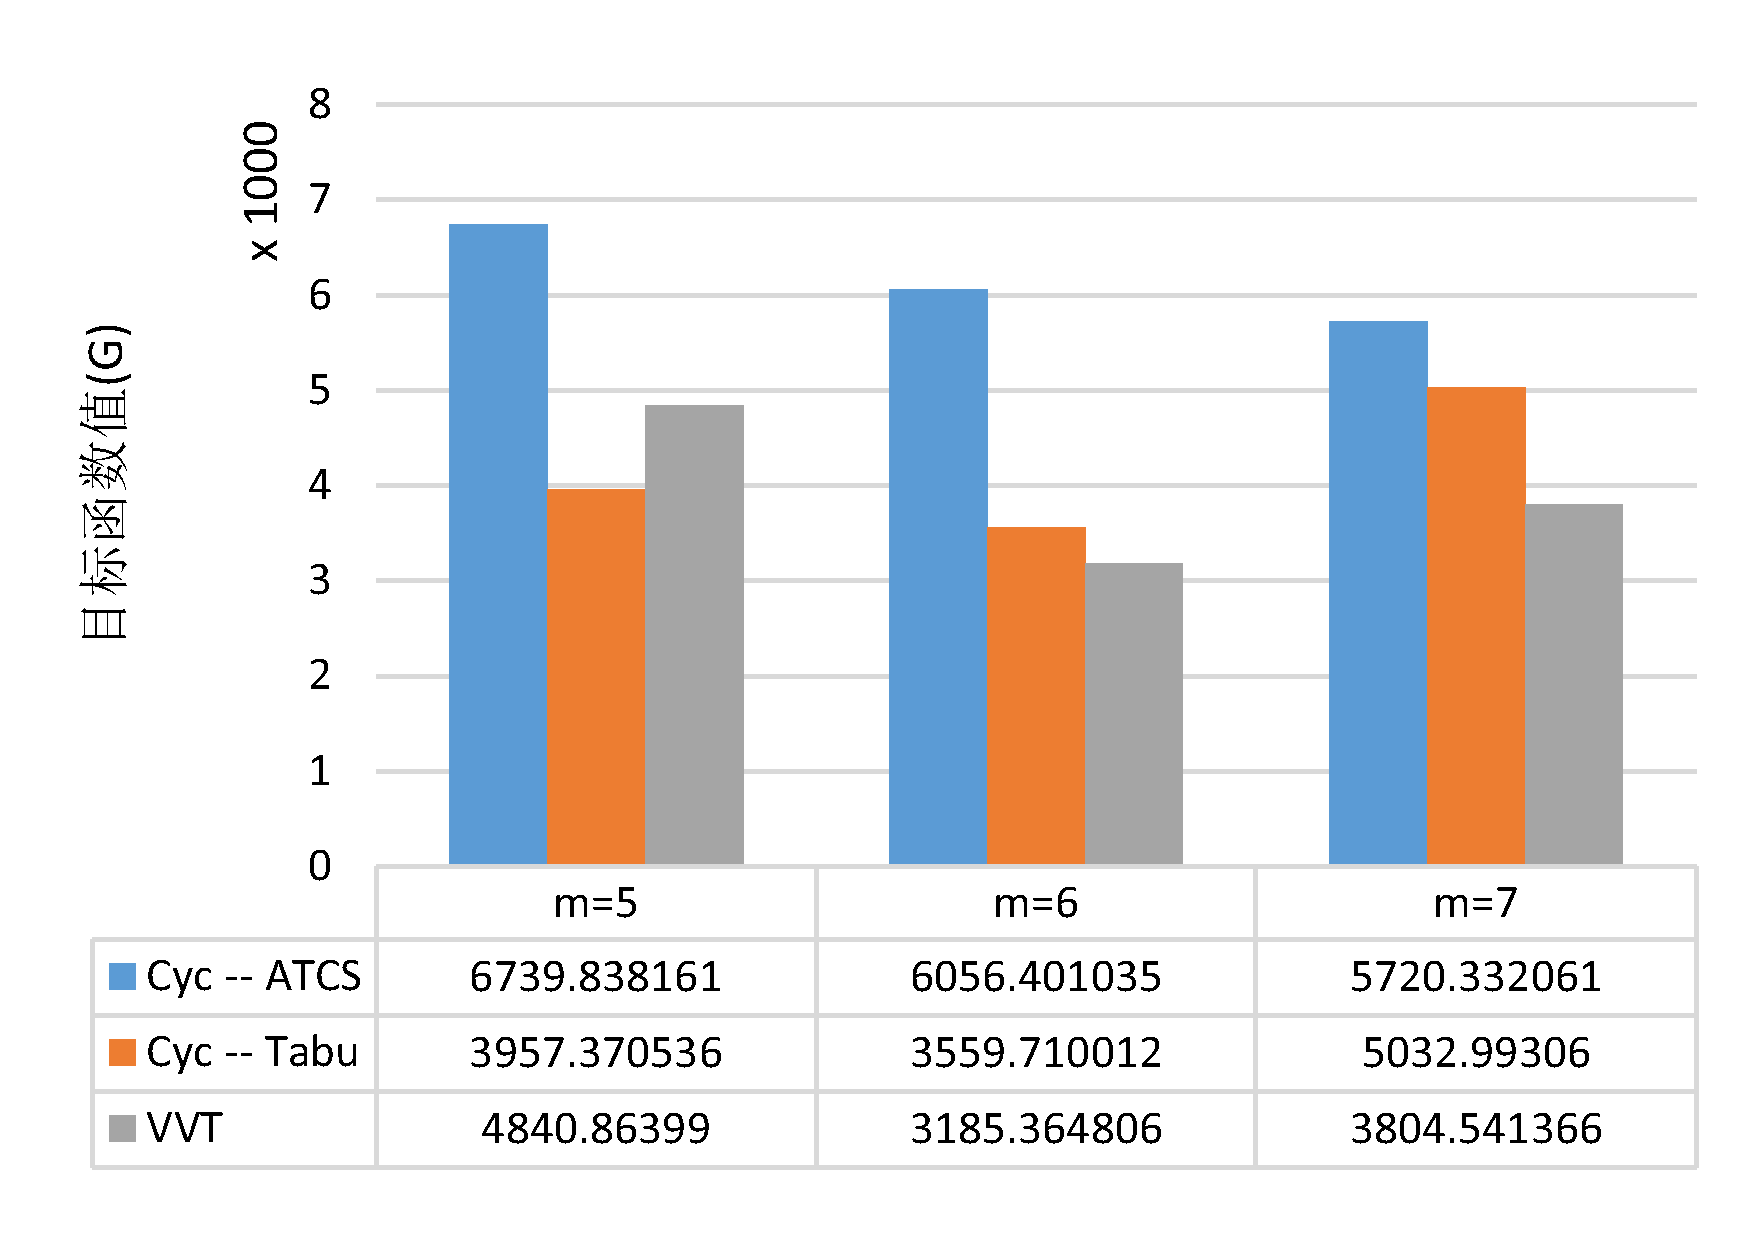
\includegraphics[height = 6cm, angle = -90]{continue_05_20}}
\subfloat[$n = 30$]{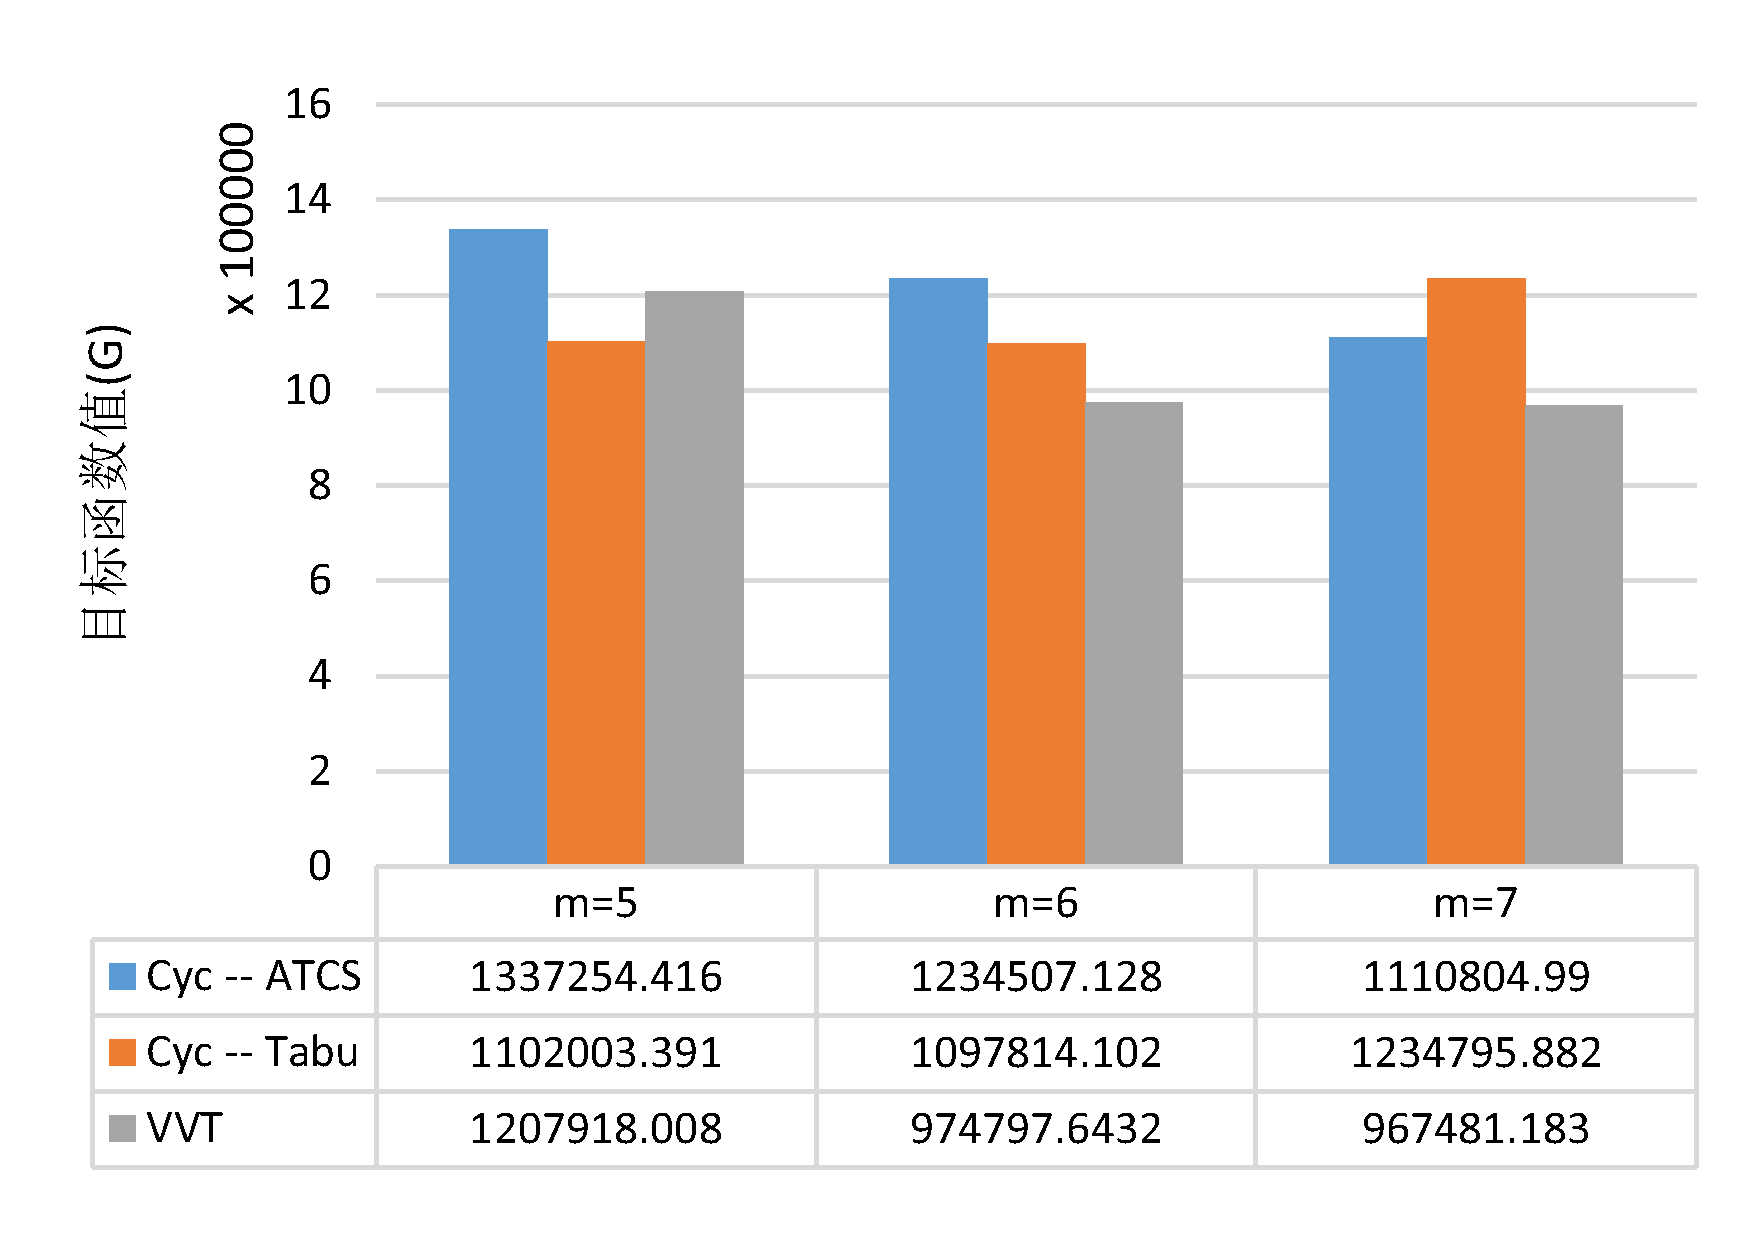
\includegraphics[height = 6cm, angle = -90]{continue_05_300}}
\subfloat[$n = 50$]{\includegraphics[height = 6cm, angle = -90]{continue_05_50}}
\subfloat[$n = 70$]{\includegraphics[height = 6cm, angle = -90]{continue_05_70}}\\
\subfloat[$n = 100$]{\includegraphics[height = 6cm, angle = -90]{continue_05_100}}
\subfloat[$n = 150$]{\includegraphics[height = 6cm, angle = -90]{continue_05_150}}
\subfloat[$n = 200$]{\includegraphics[height = 6cm, angle = -90]{continue_05_200}}
\subfloat[$n = 300$]{\includegraphics[height = 6cm, angle = -90]{continue_05_300}}\\
\subfloat[$n = 500$]{\includegraphics[height = 6cm, angle = -90]{continue_05_500}}
\subfloat[$n = 750$]{\includegraphics[height = 6cm, angle = -90]{continue_05_750}}
\subfloat[$n = 1000$]{\includegraphics[height = 6cm, angle = -90]{continue_05_1000}}
\caption{\label{fig:result5}模型$2$的Cyc -- ATCS、Cyc -- Tabu、VVT 算法求解目标函数值比较$(\lambda_1 = 0.5)$}
\end{sidewaysfigure}

\begin{sidewaysfigure}
\centering
\subfloat[$n = 20$]{\includegraphics[height = 6cm, angle = -90]{continue_06_20}}
\subfloat[$n = 30$]{\includegraphics[height = 6cm, angle = -90]{continue_06_300}}
\subfloat[$n = 50$]{\includegraphics[height = 6cm, angle = -90]{continue_06_50}}
\subfloat[$n = 70$]{\includegraphics[height = 6cm, angle = -90]{continue_06_70}}\\
\subfloat[$n = 100$]{\includegraphics[height = 6cm, angle = -90]{continue_06_100}}
\subfloat[$n = 150$]{\includegraphics[height = 6cm, angle = -90]{continue_06_150}}
\subfloat[$n = 200$]{\includegraphics[height = 6cm, angle = -90]{continue_06_200}}
\subfloat[$n = 300$]{\includegraphics[height = 6cm, angle = -90]{continue_06_300}}\\
\subfloat[$n = 500$]{\includegraphics[height = 6cm, angle = -90]{continue_06_500}}
\subfloat[$n = 750$]{\includegraphics[height = 6cm, angle = -90]{continue_06_750}}
\subfloat[$n = 1000$]{\includegraphics[height = 6cm, angle = -90]{continue_06_1000}}
\caption{\label{fig:result6}模型$2$的Cyc -- ATCS、Cyc -- Tabu、VVT 算法求解目标函数值比较$(\lambda_1 = 0.6)$}
\end{sidewaysfigure}

\begin{sidewaysfigure}
\centering
\subfloat[$n = 20$]{\includegraphics[height = 6cm, angle = -90]{Rb_04_20}}
\subfloat[$n = 30$]{\includegraphics[height = 6cm, angle = -90]{Rb_04_300}}
\subfloat[$n = 50$]{\includegraphics[height = 6cm, angle = -90]{Rb_04_50}}
\subfloat[$n = 70$]{\includegraphics[height = 6cm, angle = -90]{Rb_04_70}}\\
\subfloat[$n = 100$]{\includegraphics[height = 6cm, angle = -90]{Rb_04_100}}
\subfloat[$n = 150$]{\includegraphics[height = 6cm, angle = -90]{Rb_04_150}}
\subfloat[$n = 200$]{\includegraphics[height = 6cm, angle = -90]{Rb_04_200}}
\subfloat[$n = 300$]{\includegraphics[height = 6cm, angle = -90]{Rb_04_300}}\\
\subfloat[$n = 500$]{\includegraphics[height = 6cm, angle = -90]{Rb_04_500}}
\subfloat[$n = 750$]{\includegraphics[height = 6cm, angle = -90]{Rb_04_750}}
\subfloat[$n = 1000$]{\includegraphics[height = 6cm, angle = -90]{Rb_04_1000}}
\caption{\label{fig:result7}模型$2$的Cyc -- ATCS、Cyc -- Tabu、VVT 算法求解流水线均衡率比较$(\lambda_1 = 0.4)$}
\end{sidewaysfigure}

\begin{sidewaysfigure}
\centering
\subfloat[$n = 20$]{\includegraphics[height = 6cm, angle = -90]{Rb_05_20}}
\subfloat[$n = 30$]{\includegraphics[height = 6cm, angle = -90]{Rb_05_300}}
\subfloat[$n = 50$]{\includegraphics[height = 6cm, angle = -90]{Rb_05_50}}
\subfloat[$n = 70$]{\includegraphics[height = 6cm, angle = -90]{Rb_05_70}}\\
\subfloat[$n = 100$]{\includegraphics[height = 6cm, angle = -90]{Rb_05_100}}
\subfloat[$n = 150$]{\includegraphics[height = 6cm, angle = -90]{Rb_05_150}}
\subfloat[$n = 200$]{\includegraphics[height = 6cm, angle = -90]{Rb_05_200}}
\subfloat[$n = 300$]{\includegraphics[height = 6cm, angle = -90]{Rb_05_300}}\\
\subfloat[$n = 500$]{\includegraphics[height = 6cm, angle = -90]{Rb_05_500}}
\subfloat[$n = 750$]{\includegraphics[height = 6cm, angle = -90]{Rb_05_750}}
\subfloat[$n = 1000$]{\includegraphics[height = 6cm, angle = -90]{Rb_05_1000}}
\caption{\label{fig:result8}模型$2$的Cyc -- ATCS、Cyc -- Tabu、VVT 算法求解流水线均衡率比较$(\lambda_1 = 0.5)$}
\end{sidewaysfigure}

\begin{sidewaysfigure}
\centering
\subfloat[$n = 20$]{\includegraphics[height = 6cm, angle = -90]{Rb_06_20}}
\subfloat[$n = 30$]{\includegraphics[height = 6cm, angle = -90]{Rb_06_300}}
\subfloat[$n = 50$]{\includegraphics[height = 6cm, angle = -90]{Rb_06_50}}
\subfloat[$n = 70$]{\includegraphics[height = 6cm, angle = -90]{Rb_06_70}}\\
\subfloat[$n = 100$]{\includegraphics[height = 6cm, angle = -90]{Rb_06_100}}
\subfloat[$n = 150$]{\includegraphics[height = 6cm, angle = -90]{Rb_06_150}}
\subfloat[$n = 200$]{\includegraphics[height = 6cm, angle = -90]{Rb_06_200}}
\subfloat[$n = 300$]{\includegraphics[height = 6cm, angle = -90]{Rb_06_300}}\\
\subfloat[$n = 500$]{\includegraphics[height = 6cm, angle = -90]{Rb_06_500}}
\subfloat[$n = 750$]{\includegraphics[height = 6cm, angle = -90]{Rb_06_750}}
\subfloat[$n = 1000$]{\includegraphics[height = 6cm, angle = -90]{Rb_06_1000}}
\caption{\label{fig:result9}模型$2$的Cyc -- ATCS、Cyc -- Tabu、VVT 算法求解流水线均衡率比较$(\lambda_1 = 0.6)$}
\end{sidewaysfigure}
\chapter{算法代码}
\begin{asparaenum}
\item experiment\_data.py
\end{asparaenum}
\lstset{	basicstyle = \tiny\ttfamily,
	keywordstyle = \color{blue}\bfseries,
	stringstyle = \color{red},
	emph = {solve},
	emphstyle = \color{Green}\bfseries,
	commentstyle = \color{CadetBlue}
	}
\begin{lstlisting}[language = Python]
import sys
sys.path.append(".\\functions")
import generate
from collections import namedtuple
Item = namedtuple("Item", ['process','due','wt','wc'])

def  h(lambda1,lambda2,tardiness,completion,wt,wc):			# define the contribution of one item for the obj function
	value = lambda1*wt*tardiness + lambda2*wc*completion
	return value

def solve(input_data):
	Data = input_data.split('\n')					# load data
	n = len(Data) -1						# get the amount of items
	print n
	items = []
	for j in xrange(n):
		data = Data[j]
		parts = data.split()
		p = int(parts[0])					# get the process time
		s = int(parts[2])						# get the setup time
		d = int(parts[3])					# get the due date
		wt = int(parts[4])					# get the tardiness weights
		wc = int(parts[5])					# get the completion weights
		items.append(Item(p+s,d,wt,wc))			# combine those item data
	print 'Data loaded!'
	J = range(n)
	m = 5
	S = []
	a = []
	tl = []
	L = []
	c = [None]*n
	for l in xrange(m):
		S.append([])
		a.append(0)
		tl.append(0)
	t = 0
	f = open(".\\result\\sky",'w')
	while J:
		if 0 in a:
			l_star = a.index(0)
			p,d,wt = [],[],[]
			for j in J:				
				item = items[j]
				p.append(item.process)
				d.append(item.due)
				wt.append(item.wt)
			orderidx = generate.Idx(t,p,d,wt)
			j_star = J[orderidx.index(max(orderidx))]
			S[l_star].append(j_star)
			J.remove(j_star)
			L.append(j_star)
			tl[l_star] = t + items[j_star].process
			c[j_star] = tl[l_star]
			a[l_star] = 1
		else:
			t_star = min(tl)
			for l in xrange(m):
				if tl[l] == t_star:
					a[l] = 0
			t = t_star
	print 'initial sloution done!'
	f.write(str(S) + '\n' + str(L) + '\n' + str(c))
	f.close()


import sys
if __name__ == '__main__':
	if len(sys.argv) > 1:
		file_location = sys.argv[1].strip()
#		output = sys.argv[2].strip()
		input_data_file = open(file_location, 'r')
		input_data = ''.join(input_data_file.readlines())
		input_data_file.close()
		solve(input_data)
\end{lstlisting}
\section{456456}
\addcontentsline{toc}{section}{附录1 毕业设计文献综述}
\addcontentsline{toc}{section}{附录2 毕业设计开题报告}
\addcontentsline{toc}{section}{附录3 毕业设计外文翻译(中文译文与外文原文)}
\hspace*{7.0mm}
\hspace*{4.0mm}
\begin{minipage}[t]{95mm}
    \songti\bfseries{
    \sectionmark{附录1 毕业设计文献综述}
    附录1 毕业设计文献综述

    \vspace*{7.0mm}

    \sectionmark{附录2 毕业设计开题报告}
    附录2 毕业设计开题报告

    \vspace*{7.0mm}

    \sectionmark{附录3 毕业设计外文翻译(中文译文与外文原文)}
    附录3 毕业设计外文翻译(中文译文与外文原文)}
\end{minipage}
				% 附录

\end{document}                                  % 结束全文
